% .---------------------------------------------------------.
% | Copyright (c) 2020, Leonardo Werneck, leow155@gmail.com |
% .---------------------------------------------------------.

% Set document type, font size, and paper size
\documentclass[a4paper,11pt]{article}

%% \usepackage{xcolor}
%% \usepackage{pagecolor}

%% \pagecolor{black}
%% \color{white}

% Load all necessary packages

% Equation related packages
\usepackage{amsmath,amssymb,xfrac,bm}

% Pseudocode package
\usepackage[linesnumbered,lined,boxed]{algorithm2e}

% Figure related packages
\usepackage{graphicx,float,tikz}

% Load geometry, which allow us to configure the margins of the pages
\usepackage[left=1in,right=1in,top=0.8in,bottom=0.8in]{geometry}

% Load setspace, which allow us to set the line spacing
\usepackage{setspace}

% Load multirow, for table manipulations
\usepackage{multirow}

% Load biblatex, useful for managing the references and citations
\usepackage[backend=biber,natbib=true,style=numeric,sorting=none]{biblatex}
\addbibresource{SFcollapse1D.bib}

% Load hyperref, for colorful links
\usepackage[colorlinks=true,allcolors=blue,linktoc=page]{hyperref}

% Load hypcap, so we go to the top of figures when clicking links
\usepackage[all]{hypcap} 

% Load tcolorbox, for pretty boxes around important paragraphs
\usepackage{tcolorbox}
\tcbuselibrary{breakable} % This allow us to spam the boxes over multiple pages

% .------------------------.
% | Beginning of shortcuts |
% .------------------------.

% Code name shortcut
\newcommand{\sfcol}{\texttt{SFcollapse1D}{}}

% Change equations, tables, and figures numbering to respect sections
%% \usepackage{chngcntr}
\counterwithin{equation}{section}
\counterwithin{table}{section}
\counterwithin{figure}{section}
\counterwithin{algocf}{section}
\renewcommand{\theequation}{\arabic{section}.\arabic{equation}}
\renewcommand{\thetable}{\arabic{section}.\arabic{table}}
\renewcommand{\thefigure}{\arabic{section}.\arabic{figure}}
\renewcommand{\thealgocf}{\arabic{section}.\arabic{algocf}}

% Set useful shortcuts for greek letters and common math symbols
\renewcommand{\a}{\alpha}
\renewcommand{\b}{\beta}
\renewcommand{\d}{\delta}
\newcommand{\e}{\epsilon}
\newcommand{\g}{\gamma}
\newcommand{\s}{\sigma}
\newcommand{\D}{\Delta}
\newcommand{\gt}{\tilde{\gamma}}
\newcommand{\gDD}[2]{\g_{{#1}{#2}}}
\newcommand{\gUU}[2]{\g^{{#1}{#2}}}
\newcommand{\gtDD}[2]{\gt_{{#1}{#2}}}
\newcommand{\gtUU}[2]{\gt^{{#1}{#2}}}
\newcommand{\GDD}[2]{g_{{#1}{#2}}}
\newcommand{\GUU}[2]{g^{{#1}{#2}}}
\newcommand{\sqrtgdet}{\sqrt{\g}}
\newcommand{\sqrtGdet}{\sqrt{-g}}
\newcommand{\pd}{\partial}
\newcommand{\pdD}[1]{\pd_{{#1}}}
\newcommand{\pdU}[1]{\pd^{{#1}}}
\newcommand{\nn}{\nonumber}
\newcommand{\dt}{\Delta t}
\newcommand{\dr}{\Delta r}
\newcommand{\order}[2]{\mathcal{O}\lrpar{#1^{#2}}}
\renewcommand{\H}{\mathcal{H}}
\renewcommand{\L}{\mathcal{L}}
\newcommand{\M}{\mathcal{M}}
\renewcommand{\S}{\mathcal{S}}

% Set shortcutss for (), [], {}, and ||
\newcommand{\lrpar}[1]{\left( #1 \right)}
\newcommand{\lrsquare}[1]{\left[ #1 \right]}
\newcommand{\lrcurly}[1]{\left\{ #1 \right\}}
\newcommand{\abs}[1]{\left| #1 \right|}
\newcommand{\blrpar}[1]{\big( #1 \big)}
\newcommand{\blrsquare}[1]{\big[ #1 \big]}
\newcommand{\blrcurly}[1]{\big\{ #1 \big\}}
\newcommand{\babs}[1]{\big| #1 \big|}

% Useful shortcut to avoid typing "noindent" all over the place
\newcommand{\n}{\noindent}

% Set environment shortcuts
\newcommand{\eq}[1]{
  \begin{equation}
    #1
  \end{equation}
}
\newcommand{\spl}[1]{
  \begin{split}
    #1
  \end{split}
}
\newcommand{\al}[1]{
  \begin{align}
    #1
  \end{align}
}
\newcommand{\alat}[2]{
  \begin{alignat}{#1}
    #2
  \end{alignat}
}
\newcommand{\ctr}[1]{
  \begin{center}
    #1
  \end{center}
}
\renewcommand{\parbox}[2]{

  \vspace*{0.25in}
  
  \begin{tcolorbox}[title=Box #1,colback=blue!5!white,colframe=gray!75!black]
    #2
  \end{tcolorbox}

  \vspace*{0.25in}

}
\newcommand{\parboxbreak}[2]{
  
  \vspace*{0.25in}
  
  \begin{tcolorbox}[breakable, pad at break=1mm, before=\centering,title=Box #1,colback=blue!5!white,colframe=gray!75!black]
    #2
  \end{tcolorbox}

  \vspace*{0.25in}

}

% .------------------------.
% |    End of shortcuts    |
% .------------------------.

% Title, author, etc
\title{Gravitational collapse of a massless scalar field}
\author{Leonardo Werneck}
\date{March, 2020}

% .---------------------------.
% | Beginning of the document |
% .---------------------------.
\begin{document}

% Print the title
\maketitle

% Print the table of contents, list of figures, and list of tables
\ctr{\rule{\textwidth}{1pt}}
\tableofcontents
\ctr{\rule{\textwidth}{1pt}}
\listoffigures
\ctr{\rule{\textwidth}{1pt}}
\listoftables
\ctr{\rule{\textwidth}{1pt}}

\spacing{1.5}

\section{Introduction}

In 1993, Matt Choptuik performed numerical simulations of massless scalar fields minimally coupled to gravity and presented evidence for critical phenomena in this system~\cite{PhysRevLett.70.9}. He considered families of solutions, $\S\lrsquare{p}$, with the property that a critical parameter value, $p^{*}$, separates solutions containing black holes from those which do not. He also showed that the limit $p\to p^{*}$ is \emph{universal} (i.e. independent of the type of initial condition), with structure appearing at arbitrarily small spatiotemporal scales. Furthermore, he showed that the masses of the black holes formed in this limit obey the power law $M_{\rm BH} \propto \abs{p-p^{*}}^{\g}$, where $\g\approx0.37$ is a universal exponent.

We will present a thorough review of the techniques used by Choptuik in his seminal paper, guiding the reader through the steps required to write down a program that is able to reproduce his results. It is important, however, that the reader keep in mind that the formalism originally used by Choptuik, the ADM formalism~\cite{Arnowitt:1959ah}, is outdated and the resulting equations which are ultimately implemented are specialized to this problem, making it harder to generalize the final program for other applications. For a more extensible final program, it is recommended to use the BSSN formalism~\cite{shibata1995evolution,baumgarte1998numerical} instead. Choptuik himself has reproduced his original results using the BSSN formalism~\cite{PhysRevD.92.084037}, while many other groups have studied variations of the original problem, from which we would like to mention Baumgarte's study of aspherical initial data~\cite{Baumgarte_2018}.

We emphasize that our goal is to discuss the \emph{numerical techniques} needed to solve the problem. This means we will not derive the equations used in detail, but we will present useful references.

\section{The ADM Equations}

Here we present the equations obtained when decomposing Einstein's equations into its time and spatial componenents, known as the \emph{Arnowitt-Deser-Misner (ADM) decomposition}~\cite{Arnowitt:1959ah}. Our notation will follow that of Baumgarte and Shapiro~\cite{Baumgarte:2010ndz}.

Einstein's field equations are written in the form

\eq{
  R_{\mu\nu} - \frac{1}{2}\GDD{\mu}{\nu}R = 8\pi T_{\mu\nu}\ ,
}

\n where $\GDD{\mu}{\nu}$ is the spacetime metric, $R_{\mu\nu}$ is the Ricci tensor computed from $\GDD{\mu}{\nu}$, $R \equiv \GUU{\mu}{\nu}R_{\mu\nu}$ is the Ricci scalar, and $T_{\mu\nu}$ is the energy-momentum tensor. Note that we have chosen units such that $G_{\rm N}=1=c$, which are called \emph{geometrized units}.

The decomposition of spacetime into space plus time consists of considering spatial hypersurfaces, $\Sigma\lrpar{t}$, of constant coordinate time, $t$, which are then evolved in forward in time. The 4-metric $\GDD{\mu}{\nu}$ is written as

\eq{
  \GDD{\mu}{\nu} =
  \begin{pmatrix}
    -\a^{2} + \b_{\ell}\b^{\ell} & \b_{i}\\
    \b_{j} & \gDD{i}{j}
  \end{pmatrix}\ ,
}

\n while the inverse 4-metric is written as

\eq{
  \GUU{\mu}{\nu} =
  \begin{pmatrix}
    -\a^{-2} & \a^{-2}\b^{i}\\
    \a^{-2}\b^{j} & \gUU{i}{j} - \a^{-2}\b^{i}\b^{j}
  \end{pmatrix}\ ,
}

\n where $\a$ is known as the \emph{lapse function}, $\b$ is known as the \emph{shift vector}, and $\gDD{i}{j}$ is the ADM (or physical) 3-metric, with $\gUU{i}{j}$ its inverse.

The lapse function measures the amount of proper time that elapses while moving from a hypersurface $\Sigma\lrpar{t}$ to a hypersurface $\Sigma\lrpar{t+\dt}$, with $\dt$ a given time step. The shift vector is responsible for ``correcting'' the spatial coordinates when moving from $\Sigma\lrpar{t}$ to $\Sigma\lrpar{t+\dt}$. Consider an observer at the spatial point $(X,Y,Z)$ which lies on $\Sigma\lrpar{t}$. When we integrate in time, by moving in the normal direction towards the next hypersurface, $\Sigma\lrpar{t+\dt}$, we will arrive at the spatial point $(X^{\prime},Y^{\prime},Z^{\prime})$, which lies on $\Sigma\lrpar{t+\dt}$. Our gauge freedom allows us to folliate spacetime as we please, thus there is no guarantee that the new spatial point $(X^{\prime},Y^{\prime},Z^{\prime})$ coincides with the original point $(X,Y,Z)$. The shift vector is then used by \emph{shift} the new point $(X^{\prime},Y^{\prime},Z^{\prime})$ to the original point $(X,Y,Z)$, if necessary. It is possible, of course, to choose a folliation where this does not happen for any time, and hence, \emph{for this particular gauge choice}, $\b^{i}=0$. See figure~\ref{fig:adm_decomposition} for an illustration of the ADM decomposition.

\begin{figure}[ht]
\centering
\tikz{
	\node at (4.9,1) {$\Sigma(t+\dt)$};
	\node at (4.5,-1) {$\Sigma(t)$};
	\draw[fill,lightgray,draw=black,fill opacity=0.5] (0,-2) to [bend left] (1,-1) to [bend right] (2,0) to (4,-1) to [bend left] (3,-2) to [bend right] (2,-3) to (0,-2);
	\draw[fill,lightgray,draw=black,fill opacity=0.5] (0,0) to [bend left] (1,1) to [bend right] (2,2) to (4,1) to [bend left] (3,0) to [bend right] (2,-1) to (0,0);
	\draw[->] (1.5,-1.0) -- (1.5,1.0);
        \draw[->] (1.5,+1.0) -- (2.5,0.5);
	\draw[->,dashed] (1.5,0) to [bend left] (-0.5,-0.5) node [left] {$\a dt \,n^{\mu}$};
	\draw[dashed] (1.5,-1) -- (3.5,2) node [above right] {Line of constant $x^i=X^i$};
	\draw[->,dashed] (2,0.75) to [bend right] (1,2) node [left] {$\b^i\, dt$};
	\draw[->,dashed] (1.5,-1) to [bend right] (-0.5,-1.5) node [left] {Point $x^i = X^i$};
	\draw[fill] (1.5,-1.0) circle [radius=0.05];
        \draw[fill] (1.5,+1.0) circle [radius=0.05];
	\draw[fill] (2.5,+0.5) circle [radius=0.05];
}
\caption[Illustration of the ADM decomposition.]{Illustration of the ADM decomposition. In the picture the roles of the lapse function, $\a$, and the shift vector, $\b^i$ are depicted, and $n^{\mu}$ is the unit vector normal to the hypersurface $\Sigma(t)$. The figure can be misleading, however, because the two surfaces, $\Sigma(t)$ and $\Sigma(t+\dt)$, are drawn as exact copies of one another, while in general this is not the case.}
\label{fig:adm_decomposition}
\end{figure}

The general form of the line element is then (cf. eq. (2.123) in~\cite{Baumgarte:2010ndz})

\al{
  ds^{2} &= -\alpha^{2}dt^{2} + \gDD{i}{j}\lrpar{dx^{i} + \b^{i}dt}\lrpar{dx^{j} + \b^{j}dt} \nn\\
         &= \lrpar{-\a^{2} + \b_{\ell}\b^{\ell}}dt^{2} + 2\b_{i}dt\,dx^{i} + \gDD{i}{j}dx^{i}dx^{j}\ .
}

With the coordinate choices made above, we have that the \emph{Hamiltonian constraint} (conservation of energy), $\H$, is given by

\eq{ \H \equiv{} ^{(3)}\!R + K^{2} - K_{ij}K^{ij} - 16\pi\rho = 0\ ,\label{eq:ADMH} }

\n where $^{(3)}\!R$ is the Ricci scalar computed from $\gDD{i}{j}$, $K_{ij}$ is the extrinsic curvature of the spatial hypersurface $\Sigma$, $K\equiv \gUU{i}{j}K_{ij}$ is the trace of the extrinsic curvature, and $\rho\equiv n^{\mu}n^{\nu}T_{\mu\nu}$ is the energy density. The \emph{momentum constraints} (conservation of momentum), $\M$, are given by

\eq{ \M_{i} \equiv D_{j}K^{j}_{\ i} - D_{i}K - 8\pi S_{i} = 0\ ,\label{eq:ADMM} }

\noindent where $D_{i}$ are covariant derivatives compatible with $\gDD{i}{j}$ and $S_{i} \equiv - P^{\mu}_{\ i}n^{\nu}T_{\mu\nu}$ are \emph{momentum densities}, with $P^{\mu}_{\ \nu} \equiv \d^{\mu}_{\ \nu} + n^{\mu}n_{\nu}$ the operator which projects the spacetime components of a tensor onto the spatial hypersurface $\Sigma$.

The evolution equations for the extrinsic curvature and the metric are given by

\al{
  \pd_{t} K_{ij} &= \b^{\ell}\pd_{\ell}K_{ij} + K_{i\ell}\pd_{j}\b^{\ell} + K_{j\ell}\pd_{i}\b^{\ell} - D_{i}D_{j}\a\nn\\
                &+\a\lrpar{\,^{(3)}\!R_{ij} + K K_{ij} - 2K_{i\ell}K^{\ell}_{\ j}} + 4\pi\a\lrsquare{\g_{ij}\lrpar{S-\rho} -2S_{ij}}\ .\label{eq:ADMevoK}
}

\n and

\eq{ \pd_{t}\g_{ij} = -2\a K_{ij} + D_{i}\b_{j} + D_{j}\b_{i}\ ,\label{eq:ADMevoG} }

\n respectively. These 4 equations,~\eqref{eq:ADMH}-\eqref{eq:ADMevoG}, are the \emph{ADM equations}.

\parboxbreak{1: The ADM equations}{

  Given the 4-metric $\GDD{\mu}{\nu}$, the ADM equations are obtained by considering the decomposition

  \eq{
    \GDD{\mu}{\nu} =
    \begin{pmatrix}
      -\a^{2} + \b_{\ell}\b^{\ell} & \b_{i}\\
      \b_{j} & \gDD{i}{j}
    \end{pmatrix}\ ,
    \quad
    \GUU{\mu}{\nu} =
    \begin{pmatrix}
      -\a^{-2} & \a^{-2}\b^{i}\\
      \a^{-2}\b^{j} & \gUU{i}{j} - \a^{-2}\b^{i}\b^{j}
    \end{pmatrix}\ ,\nn
  }

  \n where $\a$ is the lapse function, $\b^{i}$ the shift vector, and $\gDD{i}{j}$ the physical spatial metric. With the choice of normal vector

  \eq{ n_{\mu} = \lrpar{-\a,0,0,0}\ ,\quad n^{\mu} = \lrpar{\a^{-1},-\a^{-1}\b^{i}}\ ,\nn}

  \n the ADM equations are written as two conservation equations (constraints) and two evolution equations. The evolution equations evolve the spatial metric and extrinsic curvature, $K_{ij}$, and are given by

  \eq{ \pd_{t}\g_{ij} = -2\a K_{ij} + D_{i}\b_{j} + D_{j}\b_{i}\ ,\nn }

  \n and

  \al{
    \pd_{t} K_{ij} &= \b^{\ell}\pd_{\ell}K_{ij} + K_{i\ell}\pd_{j}\b^{\ell} + K_{j\ell}\pd_{i}\b^{\ell} - D_{i}D_{j}\a\nn\\
                  &+\a\lrpar{\,^{(3)}\!R_{ij} + K K_{ij} - 2K_{i\ell}K^{\ell}_{\ j}} + 4\pi\a\lrsquare{\g_{ij}\lrpar{S-\rho} -2S_{ij}}\ .\nn
  }

  The Hamiltonian constraint (conservation of energy) reads

  \eq{ \H \equiv ^{(3)}\!R + K^{2} - K_{ij}K^{ij} - 16\pi\rho = 0\ ,\nn }

  \n while the momentum constraints (conservation of momentum) reads

  \eq{ \M_{i} \equiv D_{j}K^{j}_{\ i} - D_{i}K - 8\pi S_{i} = 0\ , \nn}

  \noindent where $\rho\equiv n^{\mu}n^{\nu}T_{\mu\nu}$ is the energy density and $S_{i} \equiv - P^{\mu}_{\ i}n^{\nu}T_{\mu\nu}$ are \emph{momentum densities}, with $P^{\mu}_{\ \nu} \equiv \d^{\mu}_{\ \nu} + n^{\mu}n_{\nu}$ the operator which projects the spacetime components of a tensor onto the spatial hypersurface.
}

\section{Minimally coupling a massless scalar field to gravity: the ADM+EKG system}

The gravitational collapse of a massless scalar field is studied by minimally coupling it to gravity, which is described by the action

\eq{S = \int d^{4}x \sqrtGdet \lrsquare{\frac{1}{16\pi}R - \frac{1}{2}\GUU{\mu}{\nu}\pd_{\mu}\phi\pd_{\nu}\phi}\ ,\label{eq:EKG}}

\n where $\GUU{\mu}{\nu}$ is the inverse of the physical 4-metric $\GDD{\mu}{\nu}$, $g$ is the determinant of $\GDD{\mu}{\nu}$, and $\phi$ is a massless scalar field. The energy-momentum tensor for a massless scalar field is given by

\eq{ T^{\phi}_{\mu\nu} = -\frac{2}{\sqrtGdet}\frac{\d\L_{\phi}}{\d\GUU{\mu}{\nu}} = \pd_{\mu}\phi\pd_{\nu}\phi - \frac{1}{2}\GDD{\mu}{\nu}\pd_{\a}\phi\pd^{\a}\phi\ , }

\n where $\L_{\phi} = \frac{\sqrtGdet}{2}\GUU{\mu}{\nu}\pd_{\mu}\phi\pd_{\nu}\phi$ is the Lagrangian density of a massless scalar field. We now consider the most general spherically symmetric 4-metric in the polar/radial gauge, whose line element is given by

\eq{ ds^{2} = -\a^{2}\lrpar{t,r}dt^{2} + a^{2}\lrpar{t,r}dr^{2} + r^{2}d\Omega^{2}\ , }

\n where we have chosen to write $\gDD{r}{r} = a^{2}$. The coordinate $r$ measures proper surface area, meaning that a sphere of radius $R$ has proper area $4\pi R^{2}$. The Einstein-Klein-Gordon equation, which is obtained by varying action~\eqref{eq:EKG} with respect to $\phi$, then reads

\eq{ \pd_{t}\lrpar{\frac{a}{\a}\pd_{t}\phi} = \frac{1}{r^{2}}\pd_{r}\lrpar{r^{2}\frac{\a}{a}\pd_{r}\phi}\ . }

\n At this point, Choptuik introduces the two auxiliary fields

\eq{ \Phi\lrpar{t,r} \equiv \pd_{r}\phi\lrpar{t,r}\ ,\ \Pi\lrpar{t,r} \equiv \frac{a\lrpar{t,r}}{\a\lrpar{t,r}}\pd_{t}\phi\lrpar{t,r}\ , }

\n so that the Einstein-Klein-Gordon equation can be traded by two first-order (in time and space) partial differential equations

\al{
  \pd_{t}\Phi &= \pd_{r}\lrpar{\frac{\a}{a}\Pi}\ , \label{eq:chop1}\\
  \pd_{t}\Pi  &= \frac{1}{r^{2}}\pd_{r}\lrpar{r^{2}\frac{\a}{a}\Phi} \label{eq:chop2}\ .
}

\n The energy density, $\rho = n^{\mu}n^{\nu}T^{\phi}_{\mu\nu} = \alpha^{2}T^{\phi}_{tt}$, is given by

\eq{ \rho = \frac{\Phi^{2} + \Pi^{2}}{2a^{2}}\ .}

In this coordinate system, $K = K^{r}_{\ r}$, and therefore the Hamiltonian constraint is reduced to

\eq{ \H = {}^{(3)}\!R - 16\pi\rho\ . }

\n Our gauge choice implies that the spatial Ricci scalar associated $\gDD{i}{j}$ is given by

\eq{ ^{(3)}\!R = \frac{4}{ra^{2}}\lrpar{\frac{\pd_{r}a}{a} + \frac{a^{2}-1}{2r}}\ ,}

\n which finally imply that the Hamiltonian constraint is given by

\eq{ \H = \frac{4}{ra^{2}}\lrpar{\frac{\pd_{r}a}{a} + \frac{a^{2}-1}{2r}} - 8\pi\lrpar{\frac{\Phi^{2} + \Pi^{2}}{a^{2}}} \ .}

\n Since we know that $\H=0$ \emph{analytically}, we can write the equation above as a constraint that must be satisfied at each hypersurface, namely

\eq{ \frac{\pd_{r}a}{a} + \frac{a^{2}-1}{2r} = 2\pi r\lrpar{\Phi^{2} + \Pi^{2}}\ . \label{eq:chop3} }

The last equation used by Choptuik follows from the \emph{polar slicing condition} $K^{\theta}_{\ \theta} = 0 = K^{\varphi}_{\ \varphi}$ for \emph{all} times. This implies that $\pd_{t}K_{\theta\theta} = 0$, which in turn implies the relation

\eq{ \pd_{t}K_{\theta\theta} = -D_{\theta}D_{\theta}\a + \a\, ^{(3)}\!R_{\theta\theta} + 4\pi\a\lrsquare{r^{2}\lrpar{S-\rho} - 2S_{\theta\theta}} = 0\ ,}

\n leading to the constraint equation\footnote{The following identities are useful to obtain this relation:

  \eq{
    S_{ii} = T^{\phi}_{ii}\ ,\ S = \frac{\lrpar{3\Pi^{2} - \Phi^{2}}}{2a^{2}}\ ,\ {}^{(3)}\!R_{\theta\theta} = \frac{r}{a^{3}}\pd_{r}a + \frac{a^{2}-1}{a^{2}}\ ,\ D_{\theta}D_{\theta}\a = \frac{r}{a^{2}}\pd_{r}\a\ .\nn
  }
}

\eq{ \frac{\pd_{r}\a}{\a} - \frac{\pd_{r}a}{a} - \frac{a^{2}-1}{r} = 0\ . \label{eq:chop4}}

Equations~\eqref{eq:chop1},~\eqref{eq:chop2},~\eqref{eq:chop3}, and~\eqref{eq:chop4} are equations (3)-(5) in Choptuik's original paper~\cite{PhysRevLett.70.9}.

\parboxbreak{2: The EKG+ADM equations in the radial/polar gauge}{

  The Einstein-Klein-Gordon equations in the radial/polar gauge,

  \eq{ ds^{2} = -\a^{2}\lrpar{t,r}dt^{2} + a^{2}\lrpar{t,r}dr^{2} + r^{2}d\Omega^{2}\ , \nn}

  \n are given by

  \al{
    \pd_{t}\Phi &= \pd_{r}\lrpar{\frac{\a}{a}\Pi}\ ,\nn\\
    \pd_{t}\Pi  &= \frac{1}{r^{2}}\pd_{r}\lrpar{r^{2}\frac{\a}{a}\Phi}\ . \nn
  }

  \n The equations that allow us to evolve the lapse $\a$ and the $rr$-component of the spatial metric, $\gDD{r}{r} \equiv a^{2}$, are the Hamiltonian constraint

  \eq{ \frac{\pd_{r}a}{a} + \frac{a^{2}-1}{2r} = 2\pi r\lrpar{\Phi^{2} + \Pi^{2}}\ , \nn }

  \n and the polar slicing condition $K^{\theta}_{\ \theta} = 0 = K^{\varphi}_{\ \varphi}$, which imply that $\pd_{t}K_{\theta\theta} = 0$ and thus

  \eq{ \frac{\pd_{r}\a}{\a} - \frac{\pd_{r}a}{a} - \frac{a^{2}-1}{r} = 0\ . \nn}
  
}

\section{Numerical techniques}

\subsection{Finite differences}

\begin{sloppypar}
To solve the equations inside box 2 above, we will use \emph{centered, second-order accurate finite differences} to approximate the derivatives. For a given function $f$ at the point ${(t,r)=(n\cdot\dt,j\cdot\dr)}$, where $\dt$ and $\dr$ are the time and radial step sizes, respectively, we introduce the notation $f(n\cdot\dt,j\cdot\dr) \equiv f^{n}_{j}$. Then, the derivatives of $f$ with respect to $t$ and $r$ are approximated using
\end{sloppypar}

\eq{
  \spl{
    \lrpar{\pd_{r}f}^{n}_{j} &\approx \frac{f^{n}_{j+1} - f^{n}_{j-1}}{2\dr} + \order{\dr}{2}\ ,\\
    \lrpar{\pd_{t}f}^{n}_{j} &\approx \frac{f^{n+1}_{j} - f^{n-1}_{j}}{2\dt} + \order{\dt}{2}\ .
  }
}

\n Another common technique used is to consider derivatives at the \emph{cell-centered} points $n\pm\sfrac{1}{2}$ and $j\pm\sfrac{1}{2}$, for example

\eq{
  \spl{
    \lrpar{\pd_{r}f}^{n+\sfrac{1}{2}}_{j+\sfrac{1}{2}} &\approx \frac{f^{n+\sfrac{1}{2}}_{j+1} - f^{n+\sfrac{1}{2}}_{j}}{\dr} + \order{\dr}{2}\ ,\\
    \lrpar{\pd_{r}f}^{n-\sfrac{1}{2}}_{j-\sfrac{1}{2}} &\approx \frac{f^{n-\sfrac{1}{2}}_{j} - f^{n-\sfrac{1}{2}}_{j-1}}{\dr} + \order{\dr}{2}\ ,\\
    \lrpar{\pd_{t}f}^{n+\sfrac{1}{2}}_{j+\sfrac{1}{2}} &\approx \frac{f^{n+1}_{j+\sfrac{1}{2}} - f^{n}_{j+\sfrac{1}{2}}}{\dt} + \order{\dt}{2}\ ,\\
    \lrpar{\pd_{t}f}^{n-\sfrac{1}{2}}_{j-\sfrac{1}{2}} &\approx \frac{f^{n}_{j-\sfrac{1}{2}} - f^{n-1}_{j-\sfrac{1}{2}}}{\dt} + \order{\dt}{2}\ .
  }
}

To second-order accuracy, we also consider the \emph{averaging} operations

\eq{
  \spl{
    f^{n}_{j\pm\sfrac{1}{2}} &\approx \frac{1}{2}\lrpar{f^{n}_{j\pm1} + f^{n}_{j}} + \order{\dr}{2}\ ,\\
    f^{n\pm\sfrac{1}{2}}_{j} &\approx \frac{1}{2}\lrpar{f^{n\pm1}_{j} + f^{n}_{j}} + \order{\dt}{2}\ .
  }
}

We now begin the \emph{discretization} of the evolution equations inside box 2. The discretization of the EKG equations using finite differences is given by

\al{
  \frac{\Phi^{n+1}_{j} - \Phi^{n-1}_{j}}{2\dt} &= \frac{1}{2\dr}\lrsquare{\frac{\a^{n}_{j+1}}{a^{n}_{j+1}}\Pi^{n}_{j+1} - \frac{\a^{n}_{j-1}}{a^{n}_{j-1}}\Pi^{n}_{j-1}}\ ,\\
  \frac{\Pi^{n+1}_{j}  - \Pi^{n-1}_{j}}{2\dt}  &= \frac{3}{r_{j+1}^{3} - r_{j-1}^{3}}\lrsquare{r^{2}_{j+1}\frac{\a^{n}_{j+1}}{a^{n}_{j+1}}\Pi^{n}_{j+1} - r^{2}_{i-1}\frac{\a^{n}_{j-1}}{a^{n}_{j-1}}\Pi^{n}_{j-1}}\ ,
}

\noindent where we have used the identity $r^{-2}\pd_{r} = 3\pd_{r^{3}}$ before discretizing the evolution equation for $\Pi$, in which case the step size associated with this derivative is $r^{3}_{j+1} - r^{3}_{j-1}$, where the exponent $3$ is understood to mean ``$r$ cubed'' and not ``at $n=3$''.

The discretization of the polar slicing condition is also relatively simple. First, the equation is written as

\eq{ \lrsquare{\frac{\pd_{r}\a}{\a} - \frac{\pd_{r}a}{a} - \frac{a^{2}-1}{r}}^{n+1}_{j+\sfrac{1}{2}} = 0\ .}

\n Then, using our finite differences and averaging operators, we obtain

\eq{
  \frac{\a^{n+1}_{j+1}-\a^{n+1}_{j}}{\dr}+\frac{1}{2}\lrpar{\a^{n+1}_{j+1}+\a^{n+1}_{j}}\lrcurly{\frac{1-\lrsquare{\frac{1}{2}\lrpar{a^{n+1}_{j}+a^{n+1}_{j+1}}}^2}{r_{j+\sfrac{1}{2}}}-\frac{2\lrpar{a^{n+1}_{j+1}-a^{n+1}_{j}}}{\dr\lrpar{a^{n+1}_{j+1}+a^{n+1}_{j}}}}=0\ .
}

To obtain the discretization of the Hamiltonian constraint, we first introduce a new variable

\eq{ A^{j}_{i} \equiv \ln a^{j}_{i}\ , }

\n so that we have

\al{
\frac{A^{n+1}_{j+1}-A^{n+1}_{j}}{\dr}&+\frac{\exp\lrpar{A^{n+1}_{j+1}+A^{n+1}_{j}}-1}{2r_{j+\sfrac{1}{2}}}\nn\\
&-2\pi r_{j+\sfrac{1}{2}}\lrcurly{\lrsquare{\frac{1}{2}\lrpar{\Phi^{n+1}_{j+1}+\Phi^{n+1}_{j}}}^2+\lrsquare{\frac{1}{2}\lrpar{\Pi^{n+1}_{j+1}+\Pi^{n+1}_{j}}}^2}=0\ .
}

\n This completes the discretization of the EKG+ADM system we are interested in evolving.

\parboxbreak{3: The discretization of the EKG+ADM system of equations}{

  The second-order accurate, both in time and space, discretization of the EKG+ADM system of equations, found in box 2, is

  \al{
    \frac{\Phi^{n+1}_{j} - \Phi^{n-1}_{j}}{2\dt} &= \frac{1}{2\dr}\lrsquare{\frac{\a^{n}_{j+1}}{a^{n}_{j+1}}\Pi^{n}_{j+1} - \frac{\a^{n}_{j-1}}{a^{n}_{j-1}}\Pi^{n}_{j-1}}\ ,\nn\\
    \frac{\Pi^{n+1}_{j}  - \Pi^{n-1}_{j}}{2\dt}  &= \frac{3}{r_{j+1}^{2} - r_{j-1}^{3}}\lrsquare{r^{2}_{j+1}\frac{\a^{n}_{j+1}}{a^{n}_{j+1}}\Pi^{n}_{j+1} - r^{2}_{i-1}\frac{\a^{n}_{j-1}}{a^{n}_{j-1}}\Pi^{n}_{j-1}}\ ,\nn\\
    \frac{A^{n+1}_{j+1}-A^{n+1}_{j}}{\dr}&+\frac{\exp\lrpar{A^{n+1}_{j+1}+A^{n+1}_{j}}-1}{2r_{j+\sfrac{1}{2}}}\nn\\
    &-2\pi r_{j+\sfrac{1}{2}}\lrcurly{\lrsquare{\frac{1}{2}\lrpar{\Phi^{n+1}_{j+1}+\Phi^{n+1}_{j}}}^2+\lrsquare{\frac{1}{2}\lrpar{\Pi^{n+1}_{j+1}+\Pi^{n+1}_{j}}}^2}=0\ ,\nn\\
    \frac{\a^{n+1}_{j+1}-\a^{n+1}_{j}}{\dr}&+\frac{1}{2}\lrpar{\a^{n+1}_{j+1}+\a^{n+1}_{j}}\lrcurly{\frac{1-\lrsquare{\frac{1}{2}\lrpar{a^{n+1}_{j}+a^{n+1}_{j+1}}}^2}{r_{j+\sfrac{1}{2}}}-\frac{2\lrpar{a^{n+1}_{j+1}-a^{n+1}_{j}}}{\dr\lrpar{a^{n+1}_{j+1}+a^{n+1}_{j}}}}=0\ .\nn
  }
  
}

\subsection{SinhSpherical coordinates}

We also set up the program in a way that will allow us to push the outer boundary, located at $r=r_{\max}$, a lot further out, so that we do not need to worry about spurious reflections from it. This is done by the change of variables

\eq{ r = A\frac{\sinh\lrpar{\frac{x}{w}}}{\sinh\lrpar{\frac{1}{w}}}\ ,\label{eq:sinhspherical}}

\n where $A$ and $w$ are free parameters and $x\in[0,1]$. This new coordinate system will henceforth be called \emph{SinhSpherical coordinates}. Note that $A$ corresponds to $r_{\max}$, since for $x=1$ we have $r=A$. The parameters $w$ changes the sampling density near small values of $r$. Note that while the grid structure in the $r$-coordinate is \emph{non-uniform}, being more densily sampled around $r=0$ and less densily sampled around $r=r_{\max}$, it is \emph{uniformly} sampled in the $x$-coordinate. The grid structure is illustrated in figure~\ref{fig:grid_sph_sinh}.

\begin{figure}[ht]
  \centering
  \tikz{
    % Draw the 0 and r_max lines
    \draw[dashed] (0.0,2.3) -- (0.0,-0.5) node [below] {$0$};
    
    % Grid #1: x-coordinate
    \draw[->] (0,2.0) -- (9,2.0) node [right] {$x$};
    \foreach \a in {1,...,8} {
      \draw (\a,1.9) node [below] {$x_{\a}$} -- (\a,2.1);
    }

    % Grid #2: r-coordinate, w=0.7
    \draw[->] (0.0,1.0) -- (9.0,1.0) node [right] {$r_{w=0.5}$};
    \foreach \a in {1,...,8} {
      \draw ({8.0*sinh(\a/8.0/0.5)/sinh(1.0/0.5)},0.9) node [below] {$r_{\a}$} -- ({8.0*sinh(\a/8.0/0.5)/sinh(1.0/0.5)},1.1);
    }

    % Grid #3: r-coordinate, w=0.3
    \draw[->] (0,0.0) -- (9,0.0) node [right] {$r_{w=0.3}$};
    \foreach \a in {1,...,8} {
      \draw ({8.0*sinh(\a/8.0/0.3)/sinh(1.0/0.3)},-0.1) node [below] {$r_{\a}$} -- ({8.0*sinh(\a/8.0/0.3)/sinh(1.0/0.3)},0.1);
    }
  }
  \caption[Illustration of SinhSpherical grids.]{Illustration of the grid structure for SinhSpherical coordinates. The top axis corresponds to the $x$-coordinate, which is uniformily sampled in the interval $[0,1]$. The middle and bottom axis present the corresponding $r$-coordinate when the values $w=0.5$ and $w=0.3$, respectively, are plugged into equation~\eqref{eq:sinhspherical}. We emphasize that the grid is \emph{not} uniformily sampled in the $r$-coordinate, as we can clearly see in the figure, since $\dr_{j}\equiv r_{j}-r_{j-1} < \dr_{j+1}$.}
  \label{fig:grid_sph_sinh}
\end{figure}

Since our equations are not covariant under the change of coordinates~\eqref{eq:sinhspherical}, we must adjust them appropriately. For example, we see that

\eq{ dr = \frac{A}{w}\frac{\cosh\!\lrpar{\frac{x}{w}}}{\sinh\!\lrpar{\frac{1}{w}}}dx \implies \pd_{r} = \frac{w}{A}\frac{\sinh\!\lrpar{\frac{1}{w}}}{\cosh\!\lrpar{\frac{x}{w}}} \pd_{x}\ ,}

\n so that the evolution equations now become

\al{
  \pd_{t}\Phi &= \frac{w}{A}\frac{\sinh\!\lrpar{\frac{1}{w}}}{\cosh\!\lrpar{\frac{x}{w}}} \pd_{x}\lrpar{\frac{\a}{a}\Pi}\ ,\\
  \pd_{t}\Pi  &= \frac{w}{A}\frac{\sinh\!\lrpar{\frac{1}{w}}}{\sinh^{2}\!\lrpar{\frac{x}{w}}\cosh\!\lrpar{\frac{x}{w}}} \pd_{x}\lrsquare{\sinh^{2}\!\lrpar{\frac{x}{w}}\frac{\a}{a}\Phi}\ ,\\
  \frac{\pd_{x}\a}{\a} &- \frac{\pd_{x} a}{a} - \frac{a^{2}-1}{w\tanh\!\lrpar{\frac{x}{w}}} = 0\ ,\\
  \frac{\pd_{x} a}{a} &+ \frac{a^{2}-1}{2w\tanh\!\lrpar{\frac{x}{w}}} = 2\pi\frac{A^{2}}{w\sinh^{2}\!\lrpar{\frac{1}{w}}}\sinh\!\lrpar{\frac{x}{w}}\cosh\!\lrpar{\frac{x}{w}}\lrpar{\Phi^{2} + \Pi^{2}}\ .
}

\n The discretization techniques used for the system above are identical to the ones in Spherical coordinates and will not be repeated here.

\subsection{Structure of the evolution}

The evolution of the EKG+ADM system of equations is relatively awkward since we are not allowed to use common (and simpler) integrators that follow, say, the \emph{method of lines}, such as a fourth-order Runge-Kutta (RK4) integrator. The reason for this is that both the Hamiltonian constraint and the polar slicing condition are \emph{elliptic} equations, while the EKG system is consisted of \emph{hyperbolic} equations. Simply put, the EKG system can be used to numerically evolve $\Phi$ and $\Pi$ forward in time based on their values on previous time levels, while the Hamiltonian constraint and polar slicing condition solve for $a$ and $\a$, respectively, based on information on a \emph{single} time level. This makes the integration less efficient, particularly because the Hamiltonian constraint is a non-linear equation from which we are trying to determine $A^{n+1}_{j+1}$. This means that the equation must be solved on every single gridpoint using a Newton-Raphson solver, for example, which considerably slows down the evolution and complicates the numerical algorithm. The polar slicing condition is not as difficult, it is simply an algebraic equation that must be solved for $\a^{n+1}_{j+1}$ in terms of other known quantities, but also contributes to making the integration more difficult.

During the integration process, we have access to $\lrpar{\Phi,\Pi,a,\a}$ on all spatial points, on the time levels $n$ and $n-1$. This means that a typical integration step is carried out in the following way:

\begin{enumerate}
\item Integrate $\Phi$ to the time level $n+1$
\item Integrate $\Pi$ to the time level $n+1$
\item Solve the Hamiltonian constraint to find $A$ at the time level $n+1$; compute $a$ from $A$
\item Solve the polar slicing condition to find $\a$ at the time level $n+1$
\item Set $t_{\rm new} = (n+1)\dt$. If $t_{\rm new}<t_{\max}$, go to step 1
\end{enumerate}

The summary above ignores quite a few implementation details, such as when and how to apply boundary conditions. We will go over those over the following sections.

\subsection{Boundary conditions}

\subsubsection{Inner boundary conditions}

Consider a scalar function $f(t,r)$ which is spherically symmetric. Knowing only this is enough for us to imply conditions that this function must satisfy at the origin. For example, one of the consequences of spherical symmetry is that $f\lrpar{t,-r}=f\lrpar{t,r}$, which then imply that, in particular,

\eq{ f\lrpar{t,-\dr} = f\lrpar{t,+\dr}\ . }

\n Then, we can rearrange this identity in the form of a boundary condition as

\eq{ f\lrpar{t,+\dr} - f\lrpar{t,-\dr} = 0 \implies \left.\pd_{r}f(t,r)\right|_{r=0} = 0\ . }

\n Notice that this is an \emph{inner} boundary condition which is accurate to second-order in $\dr$. A characteristic of inner boundary conditions is that we simply map a point at the boundary to another point from the grid itself. Since we are imposing the boundary condition on the derivative of the function, this is a \emph{Neumann boundary condition}. Since our primary evolved variables are all scalars, they must satisfy

\al{
  \left.\pd_{r}\phi\right|_{r=0} = 0\ ,\\
  \left.\pd_{r}\a\right|_{r=0} = 0\ ,\\
  \left.\pd_{r}a\right|_{r=0} = 0\ .
}

\n From the definitions of $\Phi$ and $\Pi$, combined with the boundary conditions above, $\Phi$ and $\Pi$ must obey

\eq{
  \Phi(t,0) = 0\ ,\ \left.\pd_{r}\Pi\right|_{r=0} = 0\ .
}

The radial metric quantity $a(t,r)$, on the other hand, is contrained at the origin due to our gauge choice. As mentioned before, the polar/radial gauge ensures that a sphere of radius $r$ has proper area $4\pi r^{2}$, and imposes the contraint

\eq{ a(t,0) = 1\ . }

\n This is the so-called ``elementary flatness condition'', which demands that the spacetime is free of conical singularities at the origin. To ensure that our gauge choice is preserved throughout the entire numerical evolution, the elementary flatness condition is implemented instead of the Neumann condition.

\parbox{4: EKG+ADM -- Inner boundary conditions}{
  For the EKG+ADM system, we apply the following \emph{inner} boundary conditions:
  \al{
    \left.\Phi\right|_{r=0} &= 0\ ,\nn\\
    \left.\pd_{r}\Pi\right|_{r=0} &= 0\ ,\nn\\
    \left.a\right|_{r=0} &= 1\ ,\nn\\
    \left.\pd_{r}\a\right|_{r=0} &= 0\ .\nn
  }
}

\subsubsection{Outer boundary conditions}

The outer boundary of our computational domain, located at $r=r_{\max}$, with $r_{\max}$ a user specified parameter, has to be treated carefully because using our centered finite difference stencils would require using points \emph{outside} our grid. Instead, we adapt our discretization scheme so that we use \emph{backwards} finite difference stencils \emph{at the outermost radial point}, namely

\eq{
  \spl{
    \lrpar{\partial_{r}f}^{n}_{j} = \frac{3f^{n}_{j} - 4f^{n}_{j-1} + f^{n}_{j-2}}{2\dr} + \order{\dr}{2}\ ,\\
    \lrpar{\partial_{t}f}^{n}_{j} = \frac{3f^{n}_{j} - 4f^{n-1}_{j} + f^{n-2}_{j}}{2\dt} + \order{\dt}{2}\ .
  }
}

For the scalar field, we will impose \emph{outgoing radiation boundary conditions}, which follow from the case where the scalar field is propagating without being coupled to gravity, i.e. the wave equation in spherical symmetry. The general solution to the spherically symmetric wave equation in spherical coordinates is

\eq{ \phi(t,r) = \frac{F(t-r) + G(t+r)}{r}\ , }

\n where $F(t-r)$ represents an \emph{outgoing} wave and $G(t+r)$ an \emph{ingoing} wave. We will demand that no extra radiation enters the computational domain at the outer boundary, which translates to the condition

\eq{ \left.\blrpar{\pd_{t}\lrsquare{r\phi(t,r)} + \pd_{r}\lrsquare{r\phi(t,r)}}\right|_{r=r_{\max}} = 0\ , }

\n at the outer boundary. This introduces a complication, since this condition cannot be written in terms of $\Phi$ and $\Pi$ alone. The easiest way to account for this is to impose the condition to $\phi$ itself, then compute $\Phi$ and $\Pi$ using their definitions. The discretization of this equation yields the outer boundary condition

\eq{ \phi^{n+1}_{J} = \lrpar{\frac{3}{\dt} + \frac{2}{r_{J}} + \frac{3}{\dr}}^{-1}\lrsquare{\frac{4\phi^{n}_{J} - \phi^{n-1}_{J}}{\dt} + \frac{4\phi^{n+1}_{J-1} - \phi^{n-1}_{J-2}}{\dr}}\ ,}

\n where the index $J$ corresponds to $r_{\max}$. Note that this is also a $\order{\dr^{2}+\dt}{2}$ approximation.

The desired outer boundary conditions for $a$ and $\a$ are

\al{
  \lim_{r\to \infty}a  &\to 1\ ,\\
  \lim_{r\to \infty}\a &\to 1\ ,
}

\n i.e. asymptotic flatness. To obtain this, we must also consider our inner boundary condition $\left.\pd_{r}\a\right|_{r=0}=0$. Note that this condition can be interpreted as implying that

\eq{ \alpha(t,0) = C\ , }

\n where $C$ is an arbitrary constant. We choose to set $C=1$ for simplicity, but this is not a physical boundary condition. The physical boundary condition is asymptotic flatness. In order to ensure that asymptotic flatness is enforced, we perform a \emph{rescaling of the lapse function} following Choptuik's prescription. First, notice that the ``evolution equation'' for the lapse function (i.e. the polar slicing condition) can be written in the form

\eq{ \a^{n}_{j+1} = \a^{n}_{j}\lrpar{\frac{1-\dr d}{1+\dr d}} \ ,}

\n where

\eq{ d = \frac{1 - \frac{b^{2}}{4}}{r_{j+\sfrac{1}{2}}} - \frac{c}{b\dr}\ ,}

\n and

\eq{ b = a^{n}_{j+1} + a^{n}_{j}\quad \text{and}\quad c = a^{n}_{j+1} - a^{n}_{j}\ .}

Notice, now, that the polar slicing condition is homogeneous in $\a$, meaning that if we multiply $\a$ \emph{on the entire hypersurface of constant time} by a constant, then the polar slicing condition is still satisfied. To ensure asymptotic flatness and that no signals propagate faster than the speed of light, we choose this constant to be

\eq{ \kappa = \min_{0\leq j\leq J}\lrpar{\frac{a^{n}_{j}}{\a^{n}_{j}}}\ . }

\n This rescaling typically sets $\a(t,r_{\max}) = a(t,r_{\max})$, which means that we are dealing with a metric that does not behave like the Schwarzschild metric, where we have $\a = a^{-1}$, except when $a=1$.

\parbox{5: EKG+ADM -- Outer boundary conditions}{
  For the EKG+ADM system, we apply the following \emph{outer} boundary conditions:
  \al{
    \phi^{n+1}_{J} &= \lrpar{\frac{3}{\dt} + \frac{2}{r_{J}} + \frac{3}{\dr}}^{-1}\lrsquare{\frac{4\phi^{n}_{J} - \phi^{n-1}_{J}}{\dt} + \frac{4\phi^{n+1}_{J-1} - \phi^{n-1}_{J-2}}{\dr}}\ ,\nn\\
    \kappa &= \min_{0\leq j\leq J}\lrpar{\frac{a^{n+1}_{j}}{\a^{n+1}_{j}}}\ ,\nn\\
    \a^{n+1}_{j} &\to \kappa\a^{n+1}_{j}\ .\nn
  }
}

\section{Solving the ADM+EKG equations numerically}

\subsection{Initial condition}

The initial condition for the scalar field is

\eq{
  \spl{
    \phi(0,r) &= \eta\exp\lrsquare{-\frac{\lrpar{r-r_{0}}^{2}}{\d^{2}}}\ ,\\
    \pd_{t}\phi(0,r) &= 0\ .
  }
  \label{eq:initial_condition_1}
}

\n Typically the parameters $r_{0}$ and $\d$ are fixed, while the parameter $\eta$, the amplitude of the initial pulse, varies on different runs of the code. This is the parameter $p$ we mentioned when discussing Choptuik's results, for which we wish to find the critical value $p^{*}=\eta_{*}$ that separates solutions with black hole formation from those with total dispersion.

In terms of $\Phi$ and $\Pi$, the inital condition reads

\eq{
  \spl{
    \Phi(0,r) &= -2\frac{\lrpar{r-r_{0}}}{\d^{2}}\eta\exp\lrsquare{-\frac{\lrpar{r-r_{0}}^{2}}{\d^{2}}}\ ,\\
    \Pi(0,r)  &= 0\ .
  }
  \label{eq:initial_condition_2}
}

\n To obtain the initial values of $a$ and $\a$ we must solve the constraints.

Although we will use the same form of the initial data used by Matt Choptuik in his PhD thesis~\cite{Choptuik_1986} and his original work~\cite{PhysRevLett.70.9}, we will choose different values for the free parameters $\lrpar{r_{0},\d}$. As pointed out by Thomas Baumgarte~\cite{Baumgarte_private}, Choptuik's choice for $\lrpar{r_{0},\d}$ lead to initial conditions which are ill-defined at the origin, as illustrated in figure~\ref{fig:origin_problem}. The radial derivative of the scalar field, $\Phi=\pd_{r}\phi$, does not go smoothly to zero at the origin, but has a ``kink'' instead. This is a consequence of imposing Neumann boundary conditions at the origin, but having an initial condition which is incompatible with this boundary condition when $r_{0}\neq 0$.

\begin{figure}[H]
  \centering
  % GNUPLOT: LaTeX picture with Postscript
\begingroup
  \makeatletter
  \providecommand\color[2][]{%
    \GenericError{(gnuplot) \space\space\space\@spaces}{%
      Package color not loaded in conjunction with
      terminal option `colourtext'%
    }{See the gnuplot documentation for explanation.%
    }{Either use 'blacktext' in gnuplot or load the package
      color.sty in LaTeX.}%
    \renewcommand\color[2][]{}%
  }%
  \providecommand\includegraphics[2][]{%
    \GenericError{(gnuplot) \space\space\space\@spaces}{%
      Package graphicx or graphics not loaded%
    }{See the gnuplot documentation for explanation.%
    }{The gnuplot epslatex terminal needs graphicx.sty or graphics.sty.}%
    \renewcommand\includegraphics[2][]{}%
  }%
  \providecommand\rotatebox[2]{#2}%
  \@ifundefined{ifGPcolor}{%
    \newif\ifGPcolor
    \GPcolorfalse
  }{}%
  \@ifundefined{ifGPblacktext}{%
    \newif\ifGPblacktext
    \GPblacktexttrue
  }{}%
  % define a \g@addto@macro without @ in the name:
  \let\gplgaddtomacro\g@addto@macro
  % define empty templates for all commands taking text:
  \gdef\gplbacktext{}%
  \gdef\gplfronttext{}%
  \makeatother
  \ifGPblacktext
    % no textcolor at all
    \def\colorrgb#1{}%
    \def\colorgray#1{}%
  \else
    % gray or color?
    \ifGPcolor
      \def\colorrgb#1{\color[rgb]{#1}}%
      \def\colorgray#1{\color[gray]{#1}}%
      \expandafter\def\csname LTw\endcsname{\color{white}}%
      \expandafter\def\csname LTb\endcsname{\color{black}}%
      \expandafter\def\csname LTa\endcsname{\color{black}}%
      \expandafter\def\csname LT0\endcsname{\color[rgb]{1,0,0}}%
      \expandafter\def\csname LT1\endcsname{\color[rgb]{0,1,0}}%
      \expandafter\def\csname LT2\endcsname{\color[rgb]{0,0,1}}%
      \expandafter\def\csname LT3\endcsname{\color[rgb]{1,0,1}}%
      \expandafter\def\csname LT4\endcsname{\color[rgb]{0,1,1}}%
      \expandafter\def\csname LT5\endcsname{\color[rgb]{1,1,0}}%
      \expandafter\def\csname LT6\endcsname{\color[rgb]{0,0,0}}%
      \expandafter\def\csname LT7\endcsname{\color[rgb]{1,0.3,0}}%
      \expandafter\def\csname LT8\endcsname{\color[rgb]{0.5,0.5,0.5}}%
    \else
      % gray
      \def\colorrgb#1{\color{black}}%
      \def\colorgray#1{\color[gray]{#1}}%
      \expandafter\def\csname LTw\endcsname{\color{white}}%
      \expandafter\def\csname LTb\endcsname{\color{black}}%
      \expandafter\def\csname LTa\endcsname{\color{black}}%
      \expandafter\def\csname LT0\endcsname{\color{black}}%
      \expandafter\def\csname LT1\endcsname{\color{black}}%
      \expandafter\def\csname LT2\endcsname{\color{black}}%
      \expandafter\def\csname LT3\endcsname{\color{black}}%
      \expandafter\def\csname LT4\endcsname{\color{black}}%
      \expandafter\def\csname LT5\endcsname{\color{black}}%
      \expandafter\def\csname LT6\endcsname{\color{black}}%
      \expandafter\def\csname LT7\endcsname{\color{black}}%
      \expandafter\def\csname LT8\endcsname{\color{black}}%
    \fi
  \fi
    \setlength{\unitlength}{0.0500bp}%
    \ifx\gptboxheight\undefined%
      \newlength{\gptboxheight}%
      \newlength{\gptboxwidth}%
      \newsavebox{\gptboxtext}%
    \fi%
    \setlength{\fboxrule}{0.5pt}%
    \setlength{\fboxsep}{1pt}%
\begin{picture}(7200.00,4320.00)%
    \gplgaddtomacro\gplbacktext{%
      \csname LTb\endcsname%%
      \put(1210,1270){\makebox(0,0)[r]{\strut{}$0$}}%
      \csname LTb\endcsname%%
      \put(1210,1836){\makebox(0,0)[r]{\strut{}$2\!\times\!10^{-8}$}}%
      \csname LTb\endcsname%%
      \put(1210,2402){\makebox(0,0)[r]{\strut{}$4\!\times\!10^{-8}$}}%
      \csname LTb\endcsname%%
      \put(1210,2967){\makebox(0,0)[r]{\strut{}$6\!\times\!10^{-8}$}}%
      \csname LTb\endcsname%%
      \put(1210,3533){\makebox(0,0)[r]{\strut{}$8\!\times\!10^{-8}$}}%
      \csname LTb\endcsname%%
      \put(2122,484){\makebox(0,0){\strut{}0.0}}%
      \csname LTb\endcsname%%
      \put(2902,484){\makebox(0,0){\strut{}0.2}}%
      \csname LTb\endcsname%%
      \put(3682,484){\makebox(0,0){\strut{}0.4}}%
      \csname LTb\endcsname%%
      \put(4463,484){\makebox(0,0){\strut{}0.6}}%
      \csname LTb\endcsname%%
      \put(5243,484){\makebox(0,0){\strut{}0.8}}%
      \csname LTb\endcsname%%
      \put(6023,484){\makebox(0,0){\strut{}1.0}}%
    }%
    \gplgaddtomacro\gplfronttext{%
      \csname LTb\endcsname%%
      \put(300,2401){\rotatebox{-270}{\makebox(0,0){\strut{}$\Phi(0,r)$}}}%
      \put(4072,154){\makebox(0,0){\strut{}$r$}}%
    }%
    \gplbacktext
    \put(0,0){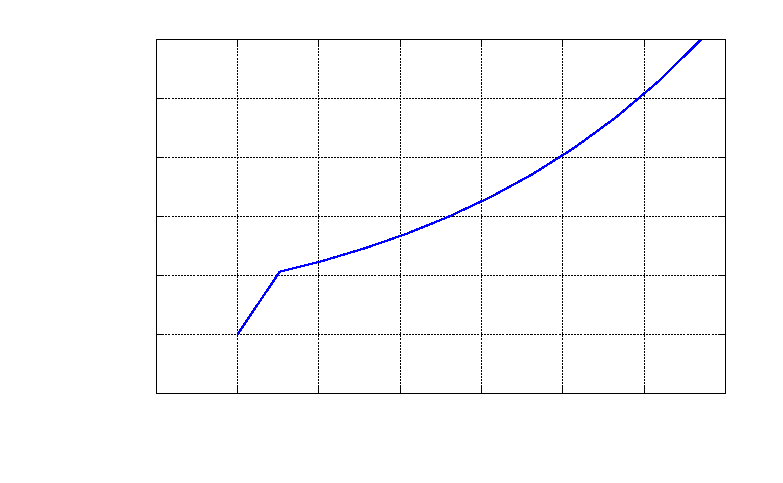
\includegraphics{resources/origin_problem}}%
    \gplfronttext
  \end{picture}%
\endgroup

  \caption[Problem with the initial condition at the origin.]{This figures shows the problem with the initial condition~\eqref{eq:initial_condition_2} when $r_{0}\neq0$. This initial condition uses the parameters $\eta=0.1$, $r_{0}=20$, and $\d=5$. There is a kink in the first derivative of the scalar field at the origin, namely the variable $\Phi$, because the initial condition is incompatible with the inner boundary condition $\left.\Phi\right|_{r=0}=0$.}
  \label{fig:origin_problem}
\end{figure}

Baumgarte has proposed a fix which he has already used himself in his studies of gravitational collapse of massless scalar fields~\cite{Baumgarte_2018}. It is a very simple fix, which consists of changing the parameters $r_{0}$ and $\delta$ appropriately. The simplest approach is to set $r_{0}=0$ and $\d=1$, which then results in the initial condition

\eq{
  \spl{
    \phi(0,r) &= \eta\exp\lrpar{-r^{2}}\ ,\\
    \Phi(0,r) &= -2r\eta\exp\lrpar{-r^{2}}\ ,\\
    \Pi(0,r) &= 0\ .
  }
  \label{eq:initial_condition_new}
}

\n This condition then guarantees that $\Phi$ is both zero and smooth at the origin. Alternatively, one could multiply $\phi(0,r)$ by $r^{n}$ with $n\geq2$, which then also guarantees that $\Phi(0,r=0)=0$.

\subsection{The {\tt SFcollapse1D} code}

We now discuss our specific implementation of this problem in the {\tt SFcollapse1D} code. Algorithm~\ref{alg:SFcollapse1D} shows the the pseudocode of {\tt SFcollapse1D}.

Some extra features of the code which are not discussed in the pseudocode are:

\begin{itemize}
  \item \textbf{Collapse of the lapse}: the code periodically checks whether or not the lapse function $\a$ has dropped below a user-specified threshold $\e_{\a}$. When the criterion $\a<\e_{\a}$ is met, the code interupts the time integratiion and characterizes the run as being in the strong field regime. We are able to infer this because around the singularity we have $\a \to 0$, which is known as the \emph{freezing of the lapse} or \emph{collapse of the lapse}.

  \item \textbf{NaN checker}: the code also periodically checks whether or not any of the evolved functions, $\lrpar{\phi,\Phi,\Pi,a,\a}$, have become NaN, ending the run if that is the case.

  \item \textbf{Run information}: integration progress is constantly printed so that the user is able to track how much of the run has already been completed. The program also shows the time elapsed during the run and estimates the amount of time required to complete the run.

  \item \textbf{Central values}: \emph{Central values} (i.e. values at $r=0$) of certain quantities, such as $\phi$, $\a$, and $\rho$, the energy density, are periodically outputted so that we can study critical phenomena.
\end{itemize}

\begin{algorithm}[H]
  \scriptsize
  \SetAlgoVlined
  \Begin(\emph{Initial condition}){
    Set the initial condition for $\phi^{0}_{j}$, $\Phi^{0}_{j}$, and $\Pi^{0}_{j}$\;
    Impose inner boundary conditions to $\Phi^{0}_{0}$, $a^{0}_{0}$, and $\a^{0}_{0}$\;
    Solve the Hamiltonian constraint to determine $a^{0}_{j}$\;
    Solve the polar slicing condition to determine $\a^{0}_{j}$\;
    Perform the rescaling of the lapse function\;
  }
  \Begin(\emph{Initial data}){
    Apply inner boundary conditions to set $\Phi^{\sfrac{1}{2}}_{0}$, $a^{\sfrac{1}{2}}_{0}$, and $\a^{\sfrac{1}{2}}_{0}$\;
    \For{$j=1$ \KwTo $N_{r}-1$}{
      \lIf{ $j=1$ }{start by computing $\phi^{\sfrac{1}{2}}_{0}$}
      Perform a half-step integration, compute $\phi^{\sfrac{1}{2}}_{j}$, $\Phi^{\sfrac{1}{2}}_{j}$, and $\Pi^{\sfrac{1}{2}}_{j}$\;
    }
    Apply outgoing radiation boundary conditions to $\phi^{\sfrac{1}{2}}_{N_{r}}$\;
    Apply inner boundary conditions to find $\Pi^{\sfrac{1}{2}}_{0}$\;
    Compute $\Phi^{\sfrac{1}{2}}_{N_{r}}$ and $\Pi^{\sfrac{1}{2}}_{N_{r}}$\;
    \For{$j=0$ \KwTo $N_{r}$}{
      Solve the Hamiltonian constraint to determine $a^{\sfrac{1}{2}}_{j}$\;
      Solve the polar slicing condition to determine $\a^{\sfrac{1}{2}}_{j}$\;
    }
    Perform the rescaling of the lapse function\;
    Apply inner boundary conditions to set $\Phi^{1}_{0}$, $a^{1}_{0}$, and $\a^{1}_{0}$\;
    \For{$j=1$ \KwTo $N_{r}-1$}{
      \lIf{ $j=1$ }{start by computing $\phi^{1}_{0}$}
      Perform a single-step integration, compute $\phi^{1}_{j}$, $\Phi^{1}_{j}$, and $\Pi^{1}_{j}$\;
    }
    Apply outgoing radiation boundary conditions to $\phi^{1}_{N_{r}}$\;
    Apply inner boundary conditions to find $\Pi^{1}_{0}$\;
    Compute $\Phi^{1}_{N_{r}}$ and $\Pi^{1}_{N_{r}}$\;
    \For{$j=0$ \KwTo $N_{r}$}{
      Solve the Hamiltonian constraint to determine $a^{1}_{j}$\;
      Solve the polar slicing condition to determine $\a^{1}_{j}$\;
    }
    Perform the rescaling of the lapse function\;
  }
  \Begin(\emph{Evolution}){
    \While{$t<t_{\rm final}$}{
      Apply inner boundary conditions to set $\Phi^{n}_{0}$, $a^{n}_{0}$, and $\a^{n}_{0}$\;
      \For{$j=1$ \KwTo $N_{r}-1$}{
        \lIf{ $j=1$ }{start by computing $\phi^{n}_{0}$}
        Compute $\phi^{n}_{j}$, $\Phi^{n}_{j}$, and $\Pi^{n}_{j}$\;
      }
      Apply outgoing radiation boundary conditions to $\phi^{n}_{N_{r}}$\;
      Apply inner boundary conditions to find $\Pi^{n}_{0}$\;
      Compute $\Phi^{n}_{N_{r}}$ and $\Pi^{n}_{N_{r}}$\;
      \For{$j=1$ \KwTo $N_{r}$}{
        Solve the Hamiltonian constraint to determine $a^{n}_{j}$\;
        Solve the polar slicing condition to determine $\a^{n}_{j}$\;
      }
      Perform the rescaling of the lapse function\;
    }
  }
  \caption{The {\tt SFcollapse1D} program's pseudocode.}
  \label{alg:SFcollapse1D}
\end{algorithm}

\subsection{Results}

\subsubsection{The different field regimes}

In this section we present results from different runs in the so-called \emph{weak} and \emph{strong} field regimes. We emphasize here that the results presented in this section were not obtained with accuracy and stability in mind, but simply to illustrate the different regimes. This means that our grid choices are not meant to be used during production runs, since they underesolve the structures that emerge once the scalar field propagates and interacts with the underlying geometry.

Throughout this section we fix the parameters $r_{0}=0$ and $\d=1$, so that $\eta$ is the parameter that will vary and allow us to obtain results in different regimes. Although we are evolving the set of variables $\lrpar{\phi,\Phi,\Pi,a,\a}$, we will be interested in looking only at the scalar field $\phi(t,r)$, the lapse function $\a(t,r)$, and the \emph{mass-aspect function}, $M(t,r)$, which is defined in analogy to the Schwarzschild metric

\eq{a^{2}(t,r) \equiv \frac{1}{1 - \frac{2M(t,r)}{r}} \implies M(t,r) = \frac{r}{2}\lrsquare{1 - \frac{1}{a^{2}(t,r)}}\ .}

\n The mass-aspect function computes the amount of mass/energy inside a sphere of radius $r$. In the limit $r\to\infty$, we have $M\to M_{\rm ADM}$, the ADM mass.

The weak field regime is obtained by choosing a value of $\eta$ which is smaller than the critical value $\eta_{*}$, and is characterized by full dispersiion. To illustrate the weak regime, we have empirically determined a value of $\eta$ that results in a spacetime which is almost flat throughout the entire run. In the run whose results are presented in figures~\ref{fig:phi_weak},~\ref{fig:alpha_weak}, and~\ref{fig:mass_weak}, we have set $\eta=0.05$. It can be seen that the metric quantities $\a$ and $a$ differ at most $\sim2\%$ from flat space, the deviation being more prominent for the lapse than the radial metric. Because of this, the backreaction from the geometry on the scalar field is negligible and we see it propagating as if it was not coupled to gravity at all, i.e. just a simple scalar wave in spherical coordinates.

\begin{figure}[H]
  \centering
  % GNUPLOT: LaTeX picture with Postscript
\begingroup
  \makeatletter
  \providecommand\color[2][]{%
    \GenericError{(gnuplot) \space\space\space\@spaces}{%
      Package color not loaded in conjunction with
      terminal option `colourtext'%
    }{See the gnuplot documentation for explanation.%
    }{Either use 'blacktext' in gnuplot or load the package
      color.sty in LaTeX.}%
    \renewcommand\color[2][]{}%
  }%
  \providecommand\includegraphics[2][]{%
    \GenericError{(gnuplot) \space\space\space\@spaces}{%
      Package graphicx or graphics not loaded%
    }{See the gnuplot documentation for explanation.%
    }{The gnuplot epslatex terminal needs graphicx.sty or graphics.sty.}%
    \renewcommand\includegraphics[2][]{}%
  }%
  \providecommand\rotatebox[2]{#2}%
  \@ifundefined{ifGPcolor}{%
    \newif\ifGPcolor
    \GPcolorfalse
  }{}%
  \@ifundefined{ifGPblacktext}{%
    \newif\ifGPblacktext
    \GPblacktexttrue
  }{}%
  % define a \g@addto@macro without @ in the name:
  \let\gplgaddtomacro\g@addto@macro
  % define empty templates for all commands taking text:
  \gdef\gplbacktext{}%
  \gdef\gplfronttext{}%
  \makeatother
  \ifGPblacktext
    % no textcolor at all
    \def\colorrgb#1{}%
    \def\colorgray#1{}%
  \else
    % gray or color?
    \ifGPcolor
      \def\colorrgb#1{\color[rgb]{#1}}%
      \def\colorgray#1{\color[gray]{#1}}%
      \expandafter\def\csname LTw\endcsname{\color{white}}%
      \expandafter\def\csname LTb\endcsname{\color{black}}%
      \expandafter\def\csname LTa\endcsname{\color{black}}%
      \expandafter\def\csname LT0\endcsname{\color[rgb]{1,0,0}}%
      \expandafter\def\csname LT1\endcsname{\color[rgb]{0,1,0}}%
      \expandafter\def\csname LT2\endcsname{\color[rgb]{0,0,1}}%
      \expandafter\def\csname LT3\endcsname{\color[rgb]{1,0,1}}%
      \expandafter\def\csname LT4\endcsname{\color[rgb]{0,1,1}}%
      \expandafter\def\csname LT5\endcsname{\color[rgb]{1,1,0}}%
      \expandafter\def\csname LT6\endcsname{\color[rgb]{0,0,0}}%
      \expandafter\def\csname LT7\endcsname{\color[rgb]{1,0.3,0}}%
      \expandafter\def\csname LT8\endcsname{\color[rgb]{0.5,0.5,0.5}}%
    \else
      % gray
      \def\colorrgb#1{\color{black}}%
      \def\colorgray#1{\color[gray]{#1}}%
      \expandafter\def\csname LTw\endcsname{\color{white}}%
      \expandafter\def\csname LTb\endcsname{\color{black}}%
      \expandafter\def\csname LTa\endcsname{\color{black}}%
      \expandafter\def\csname LT0\endcsname{\color{black}}%
      \expandafter\def\csname LT1\endcsname{\color{black}}%
      \expandafter\def\csname LT2\endcsname{\color{black}}%
      \expandafter\def\csname LT3\endcsname{\color{black}}%
      \expandafter\def\csname LT4\endcsname{\color{black}}%
      \expandafter\def\csname LT5\endcsname{\color{black}}%
      \expandafter\def\csname LT6\endcsname{\color{black}}%
      \expandafter\def\csname LT7\endcsname{\color{black}}%
      \expandafter\def\csname LT8\endcsname{\color{black}}%
    \fi
  \fi
    \setlength{\unitlength}{0.0500bp}%
    \ifx\gptboxheight\undefined%
      \newlength{\gptboxheight}%
      \newlength{\gptboxwidth}%
      \newsavebox{\gptboxtext}%
    \fi%
    \setlength{\fboxrule}{0.5pt}%
    \setlength{\fboxsep}{1pt}%
\begin{picture}(7200.00,5040.00)%
    \gplgaddtomacro\gplbacktext{%
      \csname LTb\endcsname%%
      \put(588,3706){\makebox(0,0)[r]{\strut{}-0.04}}%
      \csname LTb\endcsname%%
      \put(588,3953){\makebox(0,0)[r]{\strut{}-0.02}}%
      \csname LTb\endcsname%%
      \put(588,4199){\makebox(0,0)[r]{\strut{}0.00}}%
      \csname LTb\endcsname%%
      \put(588,4445){\makebox(0,0)[r]{\strut{}0.02}}%
      \csname LTb\endcsname%%
      \put(588,4692){\makebox(0,0)[r]{\strut{}0.04}}%
      \csname LTb\endcsname%%
      \put(896,3240){\makebox(0,0){\strut{}}}%
      \csname LTb\endcsname%%
      \put(1248,3240){\makebox(0,0){\strut{}}}%
      \csname LTb\endcsname%%
      \put(1600,3240){\makebox(0,0){\strut{}}}%
      \csname LTb\endcsname%%
      \put(1951,3240){\makebox(0,0){\strut{}}}%
      \csname LTb\endcsname%%
      \put(2303,3240){\makebox(0,0){\strut{}}}%
      \csname LTb\endcsname%%
      \put(2655,3240){\makebox(0,0){\strut{}}}%
      \put(1776,4774){\makebox(0,0){\strut{}$t = 0$}}%
    }%
    \gplgaddtomacro\gplfronttext{%
      \csname LTb\endcsname%%
      \put(-182,4199){\rotatebox{-270}{\makebox(0,0){\strut{}$\phi(t,r)$}}}%
    }%
    \gplgaddtomacro\gplbacktext{%
      \csname LTb\endcsname%%
      \put(2700,3706){\makebox(0,0)[r]{\strut{}}}%
      \csname LTb\endcsname%%
      \put(2700,3953){\makebox(0,0)[r]{\strut{}}}%
      \csname LTb\endcsname%%
      \put(2700,4199){\makebox(0,0)[r]{\strut{}}}%
      \csname LTb\endcsname%%
      \put(2700,4445){\makebox(0,0)[r]{\strut{}}}%
      \csname LTb\endcsname%%
      \put(2700,4692){\makebox(0,0)[r]{\strut{}}}%
      \csname LTb\endcsname%%
      \put(3008,3240){\makebox(0,0){\strut{}}}%
      \csname LTb\endcsname%%
      \put(3360,3240){\makebox(0,0){\strut{}}}%
      \csname LTb\endcsname%%
      \put(3712,3240){\makebox(0,0){\strut{}}}%
      \csname LTb\endcsname%%
      \put(4063,3240){\makebox(0,0){\strut{}}}%
      \csname LTb\endcsname%%
      \put(4415,3240){\makebox(0,0){\strut{}}}%
      \csname LTb\endcsname%%
      \put(4767,3240){\makebox(0,0){\strut{}}}%
      \put(3888,4774){\makebox(0,0){\strut{}$t = 0.5\times10^{3}\Delta t$}}%
    }%
    \gplgaddtomacro\gplfronttext{%
    }%
    \gplgaddtomacro\gplbacktext{%
      \csname LTb\endcsname%%
      \put(4812,3706){\makebox(0,0)[r]{\strut{}}}%
      \csname LTb\endcsname%%
      \put(4812,3953){\makebox(0,0)[r]{\strut{}}}%
      \csname LTb\endcsname%%
      \put(4812,4199){\makebox(0,0)[r]{\strut{}}}%
      \csname LTb\endcsname%%
      \put(4812,4445){\makebox(0,0)[r]{\strut{}}}%
      \csname LTb\endcsname%%
      \put(4812,4692){\makebox(0,0)[r]{\strut{}}}%
      \csname LTb\endcsname%%
      \put(5120,3240){\makebox(0,0){\strut{}}}%
      \csname LTb\endcsname%%
      \put(5472,3240){\makebox(0,0){\strut{}}}%
      \csname LTb\endcsname%%
      \put(5824,3240){\makebox(0,0){\strut{}}}%
      \csname LTb\endcsname%%
      \put(6175,3240){\makebox(0,0){\strut{}}}%
      \csname LTb\endcsname%%
      \put(6527,3240){\makebox(0,0){\strut{}}}%
      \csname LTb\endcsname%%
      \put(6879,3240){\makebox(0,0){\strut{}}}%
      \put(6000,4774){\makebox(0,0){\strut{}$t = 1.0\times10^{3}\Delta t$}}%
    }%
    \gplgaddtomacro\gplfronttext{%
    }%
    \gplgaddtomacro\gplbacktext{%
      \csname LTb\endcsname%%
      \put(588,2228){\makebox(0,0)[r]{\strut{}-0.04}}%
      \csname LTb\endcsname%%
      \put(588,2475){\makebox(0,0)[r]{\strut{}-0.02}}%
      \csname LTb\endcsname%%
      \put(588,2721){\makebox(0,0)[r]{\strut{}0.00}}%
      \csname LTb\endcsname%%
      \put(588,2967){\makebox(0,0)[r]{\strut{}0.02}}%
      \csname LTb\endcsname%%
      \put(588,3214){\makebox(0,0)[r]{\strut{}0.04}}%
      \csname LTb\endcsname%%
      \put(896,1762){\makebox(0,0){\strut{}}}%
      \csname LTb\endcsname%%
      \put(1248,1762){\makebox(0,0){\strut{}}}%
      \csname LTb\endcsname%%
      \put(1600,1762){\makebox(0,0){\strut{}}}%
      \csname LTb\endcsname%%
      \put(1951,1762){\makebox(0,0){\strut{}}}%
      \csname LTb\endcsname%%
      \put(2303,1762){\makebox(0,0){\strut{}}}%
      \csname LTb\endcsname%%
      \put(2655,1762){\makebox(0,0){\strut{}}}%
      \put(1776,3296){\makebox(0,0){\strut{}$t = 1.5\times10^{3}\Delta t$}}%
    }%
    \gplgaddtomacro\gplfronttext{%
      \csname LTb\endcsname%%
      \put(-182,2721){\rotatebox{-270}{\makebox(0,0){\strut{}$\phi(t,r)$}}}%
    }%
    \gplgaddtomacro\gplbacktext{%
      \csname LTb\endcsname%%
      \put(2700,2228){\makebox(0,0)[r]{\strut{}}}%
      \csname LTb\endcsname%%
      \put(2700,2475){\makebox(0,0)[r]{\strut{}}}%
      \csname LTb\endcsname%%
      \put(2700,2721){\makebox(0,0)[r]{\strut{}}}%
      \csname LTb\endcsname%%
      \put(2700,2967){\makebox(0,0)[r]{\strut{}}}%
      \csname LTb\endcsname%%
      \put(2700,3214){\makebox(0,0)[r]{\strut{}}}%
      \csname LTb\endcsname%%
      \put(3008,1762){\makebox(0,0){\strut{}}}%
      \csname LTb\endcsname%%
      \put(3360,1762){\makebox(0,0){\strut{}}}%
      \csname LTb\endcsname%%
      \put(3712,1762){\makebox(0,0){\strut{}}}%
      \csname LTb\endcsname%%
      \put(4063,1762){\makebox(0,0){\strut{}}}%
      \csname LTb\endcsname%%
      \put(4415,1762){\makebox(0,0){\strut{}}}%
      \csname LTb\endcsname%%
      \put(4767,1762){\makebox(0,0){\strut{}}}%
      \put(3888,3296){\makebox(0,0){\strut{}$t = 2.0\times10^{3}\Delta t$}}%
    }%
    \gplgaddtomacro\gplfronttext{%
    }%
    \gplgaddtomacro\gplbacktext{%
      \csname LTb\endcsname%%
      \put(4812,2228){\makebox(0,0)[r]{\strut{}}}%
      \csname LTb\endcsname%%
      \put(4812,2475){\makebox(0,0)[r]{\strut{}}}%
      \csname LTb\endcsname%%
      \put(4812,2721){\makebox(0,0)[r]{\strut{}}}%
      \csname LTb\endcsname%%
      \put(4812,2967){\makebox(0,0)[r]{\strut{}}}%
      \csname LTb\endcsname%%
      \put(4812,3214){\makebox(0,0)[r]{\strut{}}}%
      \csname LTb\endcsname%%
      \put(5120,1762){\makebox(0,0){\strut{}}}%
      \csname LTb\endcsname%%
      \put(5472,1762){\makebox(0,0){\strut{}}}%
      \csname LTb\endcsname%%
      \put(5824,1762){\makebox(0,0){\strut{}}}%
      \csname LTb\endcsname%%
      \put(6175,1762){\makebox(0,0){\strut{}}}%
      \csname LTb\endcsname%%
      \put(6527,1762){\makebox(0,0){\strut{}}}%
      \csname LTb\endcsname%%
      \put(6879,1762){\makebox(0,0){\strut{}}}%
      \put(6000,3296){\makebox(0,0){\strut{}$t = 2.5\times10^{3}\Delta t$}}%
    }%
    \gplgaddtomacro\gplfronttext{%
    }%
    \gplgaddtomacro\gplbacktext{%
      \csname LTb\endcsname%%
      \put(588,750){\makebox(0,0)[r]{\strut{}-0.04}}%
      \csname LTb\endcsname%%
      \put(588,997){\makebox(0,0)[r]{\strut{}-0.02}}%
      \csname LTb\endcsname%%
      \put(588,1243){\makebox(0,0)[r]{\strut{}0.00}}%
      \csname LTb\endcsname%%
      \put(588,1489){\makebox(0,0)[r]{\strut{}0.02}}%
      \csname LTb\endcsname%%
      \put(588,1736){\makebox(0,0)[r]{\strut{}0.04}}%
      \csname LTb\endcsname%%
      \put(896,284){\makebox(0,0){\strut{}$0$}}%
      \csname LTb\endcsname%%
      \put(1248,284){\makebox(0,0){\strut{}$10$}}%
      \csname LTb\endcsname%%
      \put(1600,284){\makebox(0,0){\strut{}$20$}}%
      \csname LTb\endcsname%%
      \put(1951,284){\makebox(0,0){\strut{}$30$}}%
      \csname LTb\endcsname%%
      \put(2303,284){\makebox(0,0){\strut{}$40$}}%
      \csname LTb\endcsname%%
      \put(2655,284){\makebox(0,0){\strut{}$50$}}%
      \put(1776,1818){\makebox(0,0){\strut{}$t = 3.0\times10^{3}\Delta t$}}%
    }%
    \gplgaddtomacro\gplfronttext{%
      \csname LTb\endcsname%%
      \put(-182,1243){\rotatebox{-270}{\makebox(0,0){\strut{}$\phi(t,r)$}}}%
      \put(1775,-46){\makebox(0,0){\strut{}$r$}}%
    }%
    \gplgaddtomacro\gplbacktext{%
      \csname LTb\endcsname%%
      \put(2700,750){\makebox(0,0)[r]{\strut{}}}%
      \csname LTb\endcsname%%
      \put(2700,997){\makebox(0,0)[r]{\strut{}}}%
      \csname LTb\endcsname%%
      \put(2700,1243){\makebox(0,0)[r]{\strut{}}}%
      \csname LTb\endcsname%%
      \put(2700,1489){\makebox(0,0)[r]{\strut{}}}%
      \csname LTb\endcsname%%
      \put(2700,1736){\makebox(0,0)[r]{\strut{}}}%
      \csname LTb\endcsname%%
      \put(3008,284){\makebox(0,0){\strut{}$0$}}%
      \csname LTb\endcsname%%
      \put(3360,284){\makebox(0,0){\strut{}$10$}}%
      \csname LTb\endcsname%%
      \put(3712,284){\makebox(0,0){\strut{}$20$}}%
      \csname LTb\endcsname%%
      \put(4063,284){\makebox(0,0){\strut{}$30$}}%
      \csname LTb\endcsname%%
      \put(4415,284){\makebox(0,0){\strut{}$40$}}%
      \csname LTb\endcsname%%
      \put(4767,284){\makebox(0,0){\strut{}$50$}}%
      \put(3888,1818){\makebox(0,0){\strut{}$t = 3.5\times10^{3}\Delta t$}}%
    }%
    \gplgaddtomacro\gplfronttext{%
      \csname LTb\endcsname%%
      \put(3887,-46){\makebox(0,0){\strut{}$r$}}%
    }%
    \gplgaddtomacro\gplbacktext{%
      \csname LTb\endcsname%%
      \put(4812,750){\makebox(0,0)[r]{\strut{}}}%
      \csname LTb\endcsname%%
      \put(4812,997){\makebox(0,0)[r]{\strut{}}}%
      \csname LTb\endcsname%%
      \put(4812,1243){\makebox(0,0)[r]{\strut{}}}%
      \csname LTb\endcsname%%
      \put(4812,1489){\makebox(0,0)[r]{\strut{}}}%
      \csname LTb\endcsname%%
      \put(4812,1736){\makebox(0,0)[r]{\strut{}}}%
      \csname LTb\endcsname%%
      \put(5120,284){\makebox(0,0){\strut{}$0$}}%
      \csname LTb\endcsname%%
      \put(5472,284){\makebox(0,0){\strut{}$10$}}%
      \csname LTb\endcsname%%
      \put(5824,284){\makebox(0,0){\strut{}$20$}}%
      \csname LTb\endcsname%%
      \put(6175,284){\makebox(0,0){\strut{}$30$}}%
      \csname LTb\endcsname%%
      \put(6527,284){\makebox(0,0){\strut{}$40$}}%
      \csname LTb\endcsname%%
      \put(6879,284){\makebox(0,0){\strut{}$50$}}%
      \put(6000,1818){\makebox(0,0){\strut{}$t = 4.0\times10^{3}\Delta t$}}%
    }%
    \gplgaddtomacro\gplfronttext{%
      \csname LTb\endcsname%%
      \put(5999,-46){\makebox(0,0){\strut{}$r$}}%
    }%
    \gplbacktext
    \put(0,0){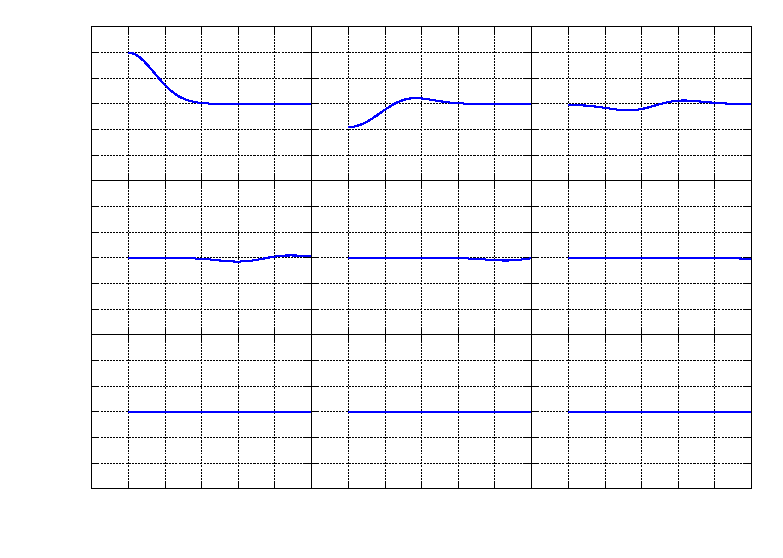
\includegraphics{scalarfield_weak}}%
    \gplfronttext
  \end{picture}%
\endgroup

  \caption[Weak field results for the scalar field $\phi(t,r)$.]{Weak field results for the scalar field $\phi(t,r)$. The parameters of the run are $\eta=0.05$, $r_{0}=0$, $\delta=1$, $r_{\max}=64$, $w=0.15$, and $N_{r}=640$.}
  \label{fig:phi_weak}
\end{figure}

\begin{figure}[H]
  \centering
  % GNUPLOT: LaTeX picture with Postscript
\begingroup
  \makeatletter
  \providecommand\color[2][]{%
    \GenericError{(gnuplot) \space\space\space\@spaces}{%
      Package color not loaded in conjunction with
      terminal option `colourtext'%
    }{See the gnuplot documentation for explanation.%
    }{Either use 'blacktext' in gnuplot or load the package
      color.sty in LaTeX.}%
    \renewcommand\color[2][]{}%
  }%
  \providecommand\includegraphics[2][]{%
    \GenericError{(gnuplot) \space\space\space\@spaces}{%
      Package graphicx or graphics not loaded%
    }{See the gnuplot documentation for explanation.%
    }{The gnuplot epslatex terminal needs graphicx.sty or graphics.sty.}%
    \renewcommand\includegraphics[2][]{}%
  }%
  \providecommand\rotatebox[2]{#2}%
  \@ifundefined{ifGPcolor}{%
    \newif\ifGPcolor
    \GPcolorfalse
  }{}%
  \@ifundefined{ifGPblacktext}{%
    \newif\ifGPblacktext
    \GPblacktexttrue
  }{}%
  % define a \g@addto@macro without @ in the name:
  \let\gplgaddtomacro\g@addto@macro
  % define empty templates for all commands taking text:
  \gdef\gplbacktext{}%
  \gdef\gplfronttext{}%
  \makeatother
  \ifGPblacktext
    % no textcolor at all
    \def\colorrgb#1{}%
    \def\colorgray#1{}%
  \else
    % gray or color?
    \ifGPcolor
      \def\colorrgb#1{\color[rgb]{#1}}%
      \def\colorgray#1{\color[gray]{#1}}%
      \expandafter\def\csname LTw\endcsname{\color{white}}%
      \expandafter\def\csname LTb\endcsname{\color{black}}%
      \expandafter\def\csname LTa\endcsname{\color{black}}%
      \expandafter\def\csname LT0\endcsname{\color[rgb]{1,0,0}}%
      \expandafter\def\csname LT1\endcsname{\color[rgb]{0,1,0}}%
      \expandafter\def\csname LT2\endcsname{\color[rgb]{0,0,1}}%
      \expandafter\def\csname LT3\endcsname{\color[rgb]{1,0,1}}%
      \expandafter\def\csname LT4\endcsname{\color[rgb]{0,1,1}}%
      \expandafter\def\csname LT5\endcsname{\color[rgb]{1,1,0}}%
      \expandafter\def\csname LT6\endcsname{\color[rgb]{0,0,0}}%
      \expandafter\def\csname LT7\endcsname{\color[rgb]{1,0.3,0}}%
      \expandafter\def\csname LT8\endcsname{\color[rgb]{0.5,0.5,0.5}}%
    \else
      % gray
      \def\colorrgb#1{\color{black}}%
      \def\colorgray#1{\color[gray]{#1}}%
      \expandafter\def\csname LTw\endcsname{\color{white}}%
      \expandafter\def\csname LTb\endcsname{\color{black}}%
      \expandafter\def\csname LTa\endcsname{\color{black}}%
      \expandafter\def\csname LT0\endcsname{\color{black}}%
      \expandafter\def\csname LT1\endcsname{\color{black}}%
      \expandafter\def\csname LT2\endcsname{\color{black}}%
      \expandafter\def\csname LT3\endcsname{\color{black}}%
      \expandafter\def\csname LT4\endcsname{\color{black}}%
      \expandafter\def\csname LT5\endcsname{\color{black}}%
      \expandafter\def\csname LT6\endcsname{\color{black}}%
      \expandafter\def\csname LT7\endcsname{\color{black}}%
      \expandafter\def\csname LT8\endcsname{\color{black}}%
    \fi
  \fi
    \setlength{\unitlength}{0.0500bp}%
    \ifx\gptboxheight\undefined%
      \newlength{\gptboxheight}%
      \newlength{\gptboxwidth}%
      \newsavebox{\gptboxtext}%
    \fi%
    \setlength{\fboxrule}{0.5pt}%
    \setlength{\fboxsep}{1pt}%
\begin{picture}(7200.00,5040.00)%
    \gplgaddtomacro\gplbacktext{%
      \csname LTb\endcsname%%
      \put(588,3706){\makebox(0,0)[r]{\strut{}0.980}}%
      \csname LTb\endcsname%%
      \put(588,3953){\makebox(0,0)[r]{\strut{}0.986}}%
      \csname LTb\endcsname%%
      \put(588,4199){\makebox(0,0)[r]{\strut{}0.991}}%
      \csname LTb\endcsname%%
      \put(588,4445){\makebox(0,0)[r]{\strut{}0.997}}%
      \csname LTb\endcsname%%
      \put(588,4692){\makebox(0,0)[r]{\strut{}1.002}}%
      \csname LTb\endcsname%%
      \put(896,3240){\makebox(0,0){\strut{}}}%
      \csname LTb\endcsname%%
      \put(1248,3240){\makebox(0,0){\strut{}}}%
      \csname LTb\endcsname%%
      \put(1600,3240){\makebox(0,0){\strut{}}}%
      \csname LTb\endcsname%%
      \put(1951,3240){\makebox(0,0){\strut{}}}%
      \csname LTb\endcsname%%
      \put(2303,3240){\makebox(0,0){\strut{}}}%
      \csname LTb\endcsname%%
      \put(2655,3240){\makebox(0,0){\strut{}}}%
      \put(1776,4774){\makebox(0,0){\strut{}$t = 0$}}%
    }%
    \gplgaddtomacro\gplfronttext{%
      \csname LTb\endcsname%%
      \put(-182,4199){\rotatebox{-270}{\makebox(0,0){\strut{}$\alpha(t,r)$}}}%
    }%
    \gplgaddtomacro\gplbacktext{%
      \csname LTb\endcsname%%
      \put(2700,3706){\makebox(0,0)[r]{\strut{}}}%
      \csname LTb\endcsname%%
      \put(2700,3953){\makebox(0,0)[r]{\strut{}}}%
      \csname LTb\endcsname%%
      \put(2700,4199){\makebox(0,0)[r]{\strut{}}}%
      \csname LTb\endcsname%%
      \put(2700,4445){\makebox(0,0)[r]{\strut{}}}%
      \csname LTb\endcsname%%
      \put(2700,4692){\makebox(0,0)[r]{\strut{}}}%
      \csname LTb\endcsname%%
      \put(3008,3240){\makebox(0,0){\strut{}}}%
      \csname LTb\endcsname%%
      \put(3360,3240){\makebox(0,0){\strut{}}}%
      \csname LTb\endcsname%%
      \put(3712,3240){\makebox(0,0){\strut{}}}%
      \csname LTb\endcsname%%
      \put(4063,3240){\makebox(0,0){\strut{}}}%
      \csname LTb\endcsname%%
      \put(4415,3240){\makebox(0,0){\strut{}}}%
      \csname LTb\endcsname%%
      \put(4767,3240){\makebox(0,0){\strut{}}}%
      \put(3888,4774){\makebox(0,0){\strut{}$t = 0.5\times10^{3}\Delta t$}}%
    }%
    \gplgaddtomacro\gplfronttext{%
    }%
    \gplgaddtomacro\gplbacktext{%
      \csname LTb\endcsname%%
      \put(4812,3706){\makebox(0,0)[r]{\strut{}}}%
      \csname LTb\endcsname%%
      \put(4812,3953){\makebox(0,0)[r]{\strut{}}}%
      \csname LTb\endcsname%%
      \put(4812,4199){\makebox(0,0)[r]{\strut{}}}%
      \csname LTb\endcsname%%
      \put(4812,4445){\makebox(0,0)[r]{\strut{}}}%
      \csname LTb\endcsname%%
      \put(4812,4692){\makebox(0,0)[r]{\strut{}}}%
      \csname LTb\endcsname%%
      \put(5120,3240){\makebox(0,0){\strut{}}}%
      \csname LTb\endcsname%%
      \put(5472,3240){\makebox(0,0){\strut{}}}%
      \csname LTb\endcsname%%
      \put(5824,3240){\makebox(0,0){\strut{}}}%
      \csname LTb\endcsname%%
      \put(6175,3240){\makebox(0,0){\strut{}}}%
      \csname LTb\endcsname%%
      \put(6527,3240){\makebox(0,0){\strut{}}}%
      \csname LTb\endcsname%%
      \put(6879,3240){\makebox(0,0){\strut{}}}%
      \put(6000,4774){\makebox(0,0){\strut{}$t = 1.0\times10^{3}\Delta t$}}%
    }%
    \gplgaddtomacro\gplfronttext{%
    }%
    \gplgaddtomacro\gplbacktext{%
      \csname LTb\endcsname%%
      \put(588,2228){\makebox(0,0)[r]{\strut{}0.980}}%
      \csname LTb\endcsname%%
      \put(588,2475){\makebox(0,0)[r]{\strut{}0.986}}%
      \csname LTb\endcsname%%
      \put(588,2721){\makebox(0,0)[r]{\strut{}0.991}}%
      \csname LTb\endcsname%%
      \put(588,2967){\makebox(0,0)[r]{\strut{}0.997}}%
      \csname LTb\endcsname%%
      \put(588,3214){\makebox(0,0)[r]{\strut{}1.002}}%
      \csname LTb\endcsname%%
      \put(896,1762){\makebox(0,0){\strut{}}}%
      \csname LTb\endcsname%%
      \put(1248,1762){\makebox(0,0){\strut{}}}%
      \csname LTb\endcsname%%
      \put(1600,1762){\makebox(0,0){\strut{}}}%
      \csname LTb\endcsname%%
      \put(1951,1762){\makebox(0,0){\strut{}}}%
      \csname LTb\endcsname%%
      \put(2303,1762){\makebox(0,0){\strut{}}}%
      \csname LTb\endcsname%%
      \put(2655,1762){\makebox(0,0){\strut{}}}%
      \put(1776,3296){\makebox(0,0){\strut{}$t = 1.5\times10^{3}\Delta t$}}%
    }%
    \gplgaddtomacro\gplfronttext{%
      \csname LTb\endcsname%%
      \put(-182,2721){\rotatebox{-270}{\makebox(0,0){\strut{}$\alpha(t,r)$}}}%
    }%
    \gplgaddtomacro\gplbacktext{%
      \csname LTb\endcsname%%
      \put(2700,2228){\makebox(0,0)[r]{\strut{}}}%
      \csname LTb\endcsname%%
      \put(2700,2475){\makebox(0,0)[r]{\strut{}}}%
      \csname LTb\endcsname%%
      \put(2700,2721){\makebox(0,0)[r]{\strut{}}}%
      \csname LTb\endcsname%%
      \put(2700,2967){\makebox(0,0)[r]{\strut{}}}%
      \csname LTb\endcsname%%
      \put(2700,3214){\makebox(0,0)[r]{\strut{}}}%
      \csname LTb\endcsname%%
      \put(3008,1762){\makebox(0,0){\strut{}}}%
      \csname LTb\endcsname%%
      \put(3360,1762){\makebox(0,0){\strut{}}}%
      \csname LTb\endcsname%%
      \put(3712,1762){\makebox(0,0){\strut{}}}%
      \csname LTb\endcsname%%
      \put(4063,1762){\makebox(0,0){\strut{}}}%
      \csname LTb\endcsname%%
      \put(4415,1762){\makebox(0,0){\strut{}}}%
      \csname LTb\endcsname%%
      \put(4767,1762){\makebox(0,0){\strut{}}}%
      \put(3888,3296){\makebox(0,0){\strut{}$t = 2.0\times10^{3}\Delta t$}}%
    }%
    \gplgaddtomacro\gplfronttext{%
    }%
    \gplgaddtomacro\gplbacktext{%
      \csname LTb\endcsname%%
      \put(4812,2228){\makebox(0,0)[r]{\strut{}}}%
      \csname LTb\endcsname%%
      \put(4812,2475){\makebox(0,0)[r]{\strut{}}}%
      \csname LTb\endcsname%%
      \put(4812,2721){\makebox(0,0)[r]{\strut{}}}%
      \csname LTb\endcsname%%
      \put(4812,2967){\makebox(0,0)[r]{\strut{}}}%
      \csname LTb\endcsname%%
      \put(4812,3214){\makebox(0,0)[r]{\strut{}}}%
      \csname LTb\endcsname%%
      \put(5120,1762){\makebox(0,0){\strut{}}}%
      \csname LTb\endcsname%%
      \put(5472,1762){\makebox(0,0){\strut{}}}%
      \csname LTb\endcsname%%
      \put(5824,1762){\makebox(0,0){\strut{}}}%
      \csname LTb\endcsname%%
      \put(6175,1762){\makebox(0,0){\strut{}}}%
      \csname LTb\endcsname%%
      \put(6527,1762){\makebox(0,0){\strut{}}}%
      \csname LTb\endcsname%%
      \put(6879,1762){\makebox(0,0){\strut{}}}%
      \put(6000,3296){\makebox(0,0){\strut{}$t = 2.5\times10^{3}\Delta t$}}%
    }%
    \gplgaddtomacro\gplfronttext{%
    }%
    \gplgaddtomacro\gplbacktext{%
      \csname LTb\endcsname%%
      \put(588,750){\makebox(0,0)[r]{\strut{}0.980}}%
      \csname LTb\endcsname%%
      \put(588,997){\makebox(0,0)[r]{\strut{}0.986}}%
      \csname LTb\endcsname%%
      \put(588,1243){\makebox(0,0)[r]{\strut{}0.991}}%
      \csname LTb\endcsname%%
      \put(588,1489){\makebox(0,0)[r]{\strut{}0.997}}%
      \csname LTb\endcsname%%
      \put(588,1736){\makebox(0,0)[r]{\strut{}1.002}}%
      \csname LTb\endcsname%%
      \put(896,284){\makebox(0,0){\strut{}$0$}}%
      \csname LTb\endcsname%%
      \put(1248,284){\makebox(0,0){\strut{}$10$}}%
      \csname LTb\endcsname%%
      \put(1600,284){\makebox(0,0){\strut{}$20$}}%
      \csname LTb\endcsname%%
      \put(1951,284){\makebox(0,0){\strut{}$30$}}%
      \csname LTb\endcsname%%
      \put(2303,284){\makebox(0,0){\strut{}$40$}}%
      \csname LTb\endcsname%%
      \put(2655,284){\makebox(0,0){\strut{}$50$}}%
      \put(1776,1818){\makebox(0,0){\strut{}$t = 3.0\times10^{3}\Delta t$}}%
    }%
    \gplgaddtomacro\gplfronttext{%
      \csname LTb\endcsname%%
      \put(-182,1243){\rotatebox{-270}{\makebox(0,0){\strut{}$\alpha(t,r)$}}}%
      \put(1775,-46){\makebox(0,0){\strut{}$r$}}%
    }%
    \gplgaddtomacro\gplbacktext{%
      \csname LTb\endcsname%%
      \put(2700,750){\makebox(0,0)[r]{\strut{}}}%
      \csname LTb\endcsname%%
      \put(2700,997){\makebox(0,0)[r]{\strut{}}}%
      \csname LTb\endcsname%%
      \put(2700,1243){\makebox(0,0)[r]{\strut{}}}%
      \csname LTb\endcsname%%
      \put(2700,1489){\makebox(0,0)[r]{\strut{}}}%
      \csname LTb\endcsname%%
      \put(2700,1736){\makebox(0,0)[r]{\strut{}}}%
      \csname LTb\endcsname%%
      \put(3008,284){\makebox(0,0){\strut{}$0$}}%
      \csname LTb\endcsname%%
      \put(3360,284){\makebox(0,0){\strut{}$10$}}%
      \csname LTb\endcsname%%
      \put(3712,284){\makebox(0,0){\strut{}$20$}}%
      \csname LTb\endcsname%%
      \put(4063,284){\makebox(0,0){\strut{}$30$}}%
      \csname LTb\endcsname%%
      \put(4415,284){\makebox(0,0){\strut{}$40$}}%
      \csname LTb\endcsname%%
      \put(4767,284){\makebox(0,0){\strut{}$50$}}%
      \put(3888,1818){\makebox(0,0){\strut{}$t = 3.5\times10^{3}\Delta t$}}%
    }%
    \gplgaddtomacro\gplfronttext{%
      \csname LTb\endcsname%%
      \put(3887,-46){\makebox(0,0){\strut{}$r$}}%
    }%
    \gplgaddtomacro\gplbacktext{%
      \csname LTb\endcsname%%
      \put(4812,750){\makebox(0,0)[r]{\strut{}}}%
      \csname LTb\endcsname%%
      \put(4812,997){\makebox(0,0)[r]{\strut{}}}%
      \csname LTb\endcsname%%
      \put(4812,1243){\makebox(0,0)[r]{\strut{}}}%
      \csname LTb\endcsname%%
      \put(4812,1489){\makebox(0,0)[r]{\strut{}}}%
      \csname LTb\endcsname%%
      \put(4812,1736){\makebox(0,0)[r]{\strut{}}}%
      \csname LTb\endcsname%%
      \put(5120,284){\makebox(0,0){\strut{}$0$}}%
      \csname LTb\endcsname%%
      \put(5472,284){\makebox(0,0){\strut{}$10$}}%
      \csname LTb\endcsname%%
      \put(5824,284){\makebox(0,0){\strut{}$20$}}%
      \csname LTb\endcsname%%
      \put(6175,284){\makebox(0,0){\strut{}$30$}}%
      \csname LTb\endcsname%%
      \put(6527,284){\makebox(0,0){\strut{}$40$}}%
      \csname LTb\endcsname%%
      \put(6879,284){\makebox(0,0){\strut{}$50$}}%
      \put(6000,1818){\makebox(0,0){\strut{}$t = 4.0\times10^{3}\Delta t$}}%
    }%
    \gplgaddtomacro\gplfronttext{%
      \csname LTb\endcsname%%
      \put(5999,-46){\makebox(0,0){\strut{}$r$}}%
    }%
    \gplbacktext
    \put(0,0){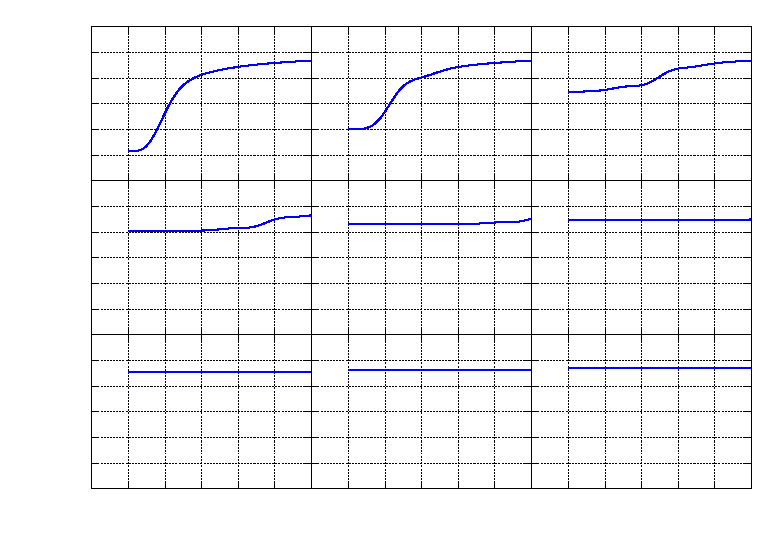
\includegraphics{alpha_weak}}%
    \gplfronttext
  \end{picture}%
\endgroup

  \caption[Weak field results for the lapse function $\a(t,r)$.]{Weak field results for the lapse function $\a(t,r)$. The parameters of the run are $\eta=0.05$, $r_{0}=0$, $\delta=1$, $r_{\max}=64$, $w=0.15$, and $N_{r}=640$.}
  \label{fig:alpha_weak}
\end{figure}

\begin{figure}[H]
  \centering
  % GNUPLOT: LaTeX picture with Postscript
\begingroup
  \makeatletter
  \providecommand\color[2][]{%
    \GenericError{(gnuplot) \space\space\space\@spaces}{%
      Package color not loaded in conjunction with
      terminal option `colourtext'%
    }{See the gnuplot documentation for explanation.%
    }{Either use 'blacktext' in gnuplot or load the package
      color.sty in LaTeX.}%
    \renewcommand\color[2][]{}%
  }%
  \providecommand\includegraphics[2][]{%
    \GenericError{(gnuplot) \space\space\space\@spaces}{%
      Package graphicx or graphics not loaded%
    }{See the gnuplot documentation for explanation.%
    }{The gnuplot epslatex terminal needs graphicx.sty or graphics.sty.}%
    \renewcommand\includegraphics[2][]{}%
  }%
  \providecommand\rotatebox[2]{#2}%
  \@ifundefined{ifGPcolor}{%
    \newif\ifGPcolor
    \GPcolorfalse
  }{}%
  \@ifundefined{ifGPblacktext}{%
    \newif\ifGPblacktext
    \GPblacktexttrue
  }{}%
  % define a \g@addto@macro without @ in the name:
  \let\gplgaddtomacro\g@addto@macro
  % define empty templates for all commands taking text:
  \gdef\gplbacktext{}%
  \gdef\gplfronttext{}%
  \makeatother
  \ifGPblacktext
    % no textcolor at all
    \def\colorrgb#1{}%
    \def\colorgray#1{}%
  \else
    % gray or color?
    \ifGPcolor
      \def\colorrgb#1{\color[rgb]{#1}}%
      \def\colorgray#1{\color[gray]{#1}}%
      \expandafter\def\csname LTw\endcsname{\color{white}}%
      \expandafter\def\csname LTb\endcsname{\color{black}}%
      \expandafter\def\csname LTa\endcsname{\color{black}}%
      \expandafter\def\csname LT0\endcsname{\color[rgb]{1,0,0}}%
      \expandafter\def\csname LT1\endcsname{\color[rgb]{0,1,0}}%
      \expandafter\def\csname LT2\endcsname{\color[rgb]{0,0,1}}%
      \expandafter\def\csname LT3\endcsname{\color[rgb]{1,0,1}}%
      \expandafter\def\csname LT4\endcsname{\color[rgb]{0,1,1}}%
      \expandafter\def\csname LT5\endcsname{\color[rgb]{1,1,0}}%
      \expandafter\def\csname LT6\endcsname{\color[rgb]{0,0,0}}%
      \expandafter\def\csname LT7\endcsname{\color[rgb]{1,0.3,0}}%
      \expandafter\def\csname LT8\endcsname{\color[rgb]{0.5,0.5,0.5}}%
    \else
      % gray
      \def\colorrgb#1{\color{black}}%
      \def\colorgray#1{\color[gray]{#1}}%
      \expandafter\def\csname LTw\endcsname{\color{white}}%
      \expandafter\def\csname LTb\endcsname{\color{black}}%
      \expandafter\def\csname LTa\endcsname{\color{black}}%
      \expandafter\def\csname LT0\endcsname{\color{black}}%
      \expandafter\def\csname LT1\endcsname{\color{black}}%
      \expandafter\def\csname LT2\endcsname{\color{black}}%
      \expandafter\def\csname LT3\endcsname{\color{black}}%
      \expandafter\def\csname LT4\endcsname{\color{black}}%
      \expandafter\def\csname LT5\endcsname{\color{black}}%
      \expandafter\def\csname LT6\endcsname{\color{black}}%
      \expandafter\def\csname LT7\endcsname{\color{black}}%
      \expandafter\def\csname LT8\endcsname{\color{black}}%
    \fi
  \fi
    \setlength{\unitlength}{0.0500bp}%
    \ifx\gptboxheight\undefined%
      \newlength{\gptboxheight}%
      \newlength{\gptboxwidth}%
      \newsavebox{\gptboxtext}%
    \fi%
    \setlength{\fboxrule}{0.5pt}%
    \setlength{\fboxsep}{1pt}%
\begin{picture}(7200.00,5040.00)%
    \gplgaddtomacro\gplbacktext{%
      \csname LTb\endcsname%%
      \put(588,3706){\makebox(0,0)[r]{\strut{}0.000}}%
      \csname LTb\endcsname%%
      \put(588,3953){\makebox(0,0)[r]{\strut{}0.018}}%
      \csname LTb\endcsname%%
      \put(588,4199){\makebox(0,0)[r]{\strut{}0.035}}%
      \csname LTb\endcsname%%
      \put(588,4445){\makebox(0,0)[r]{\strut{}0.053}}%
      \csname LTb\endcsname%%
      \put(588,4692){\makebox(0,0)[r]{\strut{}0.070}}%
      \csname LTb\endcsname%%
      \put(896,3240){\makebox(0,0){\strut{}}}%
      \csname LTb\endcsname%%
      \put(1248,3240){\makebox(0,0){\strut{}}}%
      \csname LTb\endcsname%%
      \put(1600,3240){\makebox(0,0){\strut{}}}%
      \csname LTb\endcsname%%
      \put(1951,3240){\makebox(0,0){\strut{}}}%
      \csname LTb\endcsname%%
      \put(2303,3240){\makebox(0,0){\strut{}}}%
      \csname LTb\endcsname%%
      \put(2655,3240){\makebox(0,0){\strut{}}}%
      \put(1776,4774){\makebox(0,0){\strut{}$t = 0$}}%
    }%
    \gplgaddtomacro\gplfronttext{%
      \csname LTb\endcsname%%
      \put(-182,4199){\rotatebox{-270}{\makebox(0,0){\strut{}$M(t,r)$}}}%
    }%
    \gplgaddtomacro\gplbacktext{%
      \csname LTb\endcsname%%
      \put(2700,3706){\makebox(0,0)[r]{\strut{}}}%
      \csname LTb\endcsname%%
      \put(2700,3953){\makebox(0,0)[r]{\strut{}}}%
      \csname LTb\endcsname%%
      \put(2700,4199){\makebox(0,0)[r]{\strut{}}}%
      \csname LTb\endcsname%%
      \put(2700,4445){\makebox(0,0)[r]{\strut{}}}%
      \csname LTb\endcsname%%
      \put(2700,4692){\makebox(0,0)[r]{\strut{}}}%
      \csname LTb\endcsname%%
      \put(3008,3240){\makebox(0,0){\strut{}}}%
      \csname LTb\endcsname%%
      \put(3360,3240){\makebox(0,0){\strut{}}}%
      \csname LTb\endcsname%%
      \put(3712,3240){\makebox(0,0){\strut{}}}%
      \csname LTb\endcsname%%
      \put(4063,3240){\makebox(0,0){\strut{}}}%
      \csname LTb\endcsname%%
      \put(4415,3240){\makebox(0,0){\strut{}}}%
      \csname LTb\endcsname%%
      \put(4767,3240){\makebox(0,0){\strut{}}}%
      \put(3888,4774){\makebox(0,0){\strut{}$t = 0.5\times10^{3}\Delta t$}}%
    }%
    \gplgaddtomacro\gplfronttext{%
    }%
    \gplgaddtomacro\gplbacktext{%
      \csname LTb\endcsname%%
      \put(4812,3706){\makebox(0,0)[r]{\strut{}}}%
      \csname LTb\endcsname%%
      \put(4812,3953){\makebox(0,0)[r]{\strut{}}}%
      \csname LTb\endcsname%%
      \put(4812,4199){\makebox(0,0)[r]{\strut{}}}%
      \csname LTb\endcsname%%
      \put(4812,4445){\makebox(0,0)[r]{\strut{}}}%
      \csname LTb\endcsname%%
      \put(4812,4692){\makebox(0,0)[r]{\strut{}}}%
      \csname LTb\endcsname%%
      \put(5120,3240){\makebox(0,0){\strut{}}}%
      \csname LTb\endcsname%%
      \put(5472,3240){\makebox(0,0){\strut{}}}%
      \csname LTb\endcsname%%
      \put(5824,3240){\makebox(0,0){\strut{}}}%
      \csname LTb\endcsname%%
      \put(6175,3240){\makebox(0,0){\strut{}}}%
      \csname LTb\endcsname%%
      \put(6527,3240){\makebox(0,0){\strut{}}}%
      \csname LTb\endcsname%%
      \put(6879,3240){\makebox(0,0){\strut{}}}%
      \put(6000,4774){\makebox(0,0){\strut{}$t = 1.0\times10^{3}\Delta t$}}%
    }%
    \gplgaddtomacro\gplfronttext{%
    }%
    \gplgaddtomacro\gplbacktext{%
      \csname LTb\endcsname%%
      \put(588,2228){\makebox(0,0)[r]{\strut{}0.000}}%
      \csname LTb\endcsname%%
      \put(588,2475){\makebox(0,0)[r]{\strut{}0.018}}%
      \csname LTb\endcsname%%
      \put(588,2721){\makebox(0,0)[r]{\strut{}0.035}}%
      \csname LTb\endcsname%%
      \put(588,2967){\makebox(0,0)[r]{\strut{}0.053}}%
      \csname LTb\endcsname%%
      \put(588,3214){\makebox(0,0)[r]{\strut{}0.070}}%
      \csname LTb\endcsname%%
      \put(896,1762){\makebox(0,0){\strut{}}}%
      \csname LTb\endcsname%%
      \put(1248,1762){\makebox(0,0){\strut{}}}%
      \csname LTb\endcsname%%
      \put(1600,1762){\makebox(0,0){\strut{}}}%
      \csname LTb\endcsname%%
      \put(1951,1762){\makebox(0,0){\strut{}}}%
      \csname LTb\endcsname%%
      \put(2303,1762){\makebox(0,0){\strut{}}}%
      \csname LTb\endcsname%%
      \put(2655,1762){\makebox(0,0){\strut{}}}%
      \put(1776,3296){\makebox(0,0){\strut{}$t = 1.5\times10^{3}\Delta t$}}%
    }%
    \gplgaddtomacro\gplfronttext{%
      \csname LTb\endcsname%%
      \put(-182,2721){\rotatebox{-270}{\makebox(0,0){\strut{}$M(t,r)$}}}%
    }%
    \gplgaddtomacro\gplbacktext{%
      \csname LTb\endcsname%%
      \put(2700,2228){\makebox(0,0)[r]{\strut{}}}%
      \csname LTb\endcsname%%
      \put(2700,2475){\makebox(0,0)[r]{\strut{}}}%
      \csname LTb\endcsname%%
      \put(2700,2721){\makebox(0,0)[r]{\strut{}}}%
      \csname LTb\endcsname%%
      \put(2700,2967){\makebox(0,0)[r]{\strut{}}}%
      \csname LTb\endcsname%%
      \put(2700,3214){\makebox(0,0)[r]{\strut{}}}%
      \csname LTb\endcsname%%
      \put(3008,1762){\makebox(0,0){\strut{}}}%
      \csname LTb\endcsname%%
      \put(3360,1762){\makebox(0,0){\strut{}}}%
      \csname LTb\endcsname%%
      \put(3712,1762){\makebox(0,0){\strut{}}}%
      \csname LTb\endcsname%%
      \put(4063,1762){\makebox(0,0){\strut{}}}%
      \csname LTb\endcsname%%
      \put(4415,1762){\makebox(0,0){\strut{}}}%
      \csname LTb\endcsname%%
      \put(4767,1762){\makebox(0,0){\strut{}}}%
      \put(3888,3296){\makebox(0,0){\strut{}$t = 2.0\times10^{3}\Delta t$}}%
    }%
    \gplgaddtomacro\gplfronttext{%
    }%
    \gplgaddtomacro\gplbacktext{%
      \csname LTb\endcsname%%
      \put(4812,2228){\makebox(0,0)[r]{\strut{}}}%
      \csname LTb\endcsname%%
      \put(4812,2475){\makebox(0,0)[r]{\strut{}}}%
      \csname LTb\endcsname%%
      \put(4812,2721){\makebox(0,0)[r]{\strut{}}}%
      \csname LTb\endcsname%%
      \put(4812,2967){\makebox(0,0)[r]{\strut{}}}%
      \csname LTb\endcsname%%
      \put(4812,3214){\makebox(0,0)[r]{\strut{}}}%
      \csname LTb\endcsname%%
      \put(5120,1762){\makebox(0,0){\strut{}}}%
      \csname LTb\endcsname%%
      \put(5472,1762){\makebox(0,0){\strut{}}}%
      \csname LTb\endcsname%%
      \put(5824,1762){\makebox(0,0){\strut{}}}%
      \csname LTb\endcsname%%
      \put(6175,1762){\makebox(0,0){\strut{}}}%
      \csname LTb\endcsname%%
      \put(6527,1762){\makebox(0,0){\strut{}}}%
      \csname LTb\endcsname%%
      \put(6879,1762){\makebox(0,0){\strut{}}}%
      \put(6000,3296){\makebox(0,0){\strut{}$t = 2.5\times10^{3}\Delta t$}}%
    }%
    \gplgaddtomacro\gplfronttext{%
    }%
    \gplgaddtomacro\gplbacktext{%
      \csname LTb\endcsname%%
      \put(588,750){\makebox(0,0)[r]{\strut{}0.000}}%
      \csname LTb\endcsname%%
      \put(588,997){\makebox(0,0)[r]{\strut{}0.018}}%
      \csname LTb\endcsname%%
      \put(588,1243){\makebox(0,0)[r]{\strut{}0.035}}%
      \csname LTb\endcsname%%
      \put(588,1489){\makebox(0,0)[r]{\strut{}0.053}}%
      \csname LTb\endcsname%%
      \put(588,1736){\makebox(0,0)[r]{\strut{}0.070}}%
      \csname LTb\endcsname%%
      \put(896,284){\makebox(0,0){\strut{}$0$}}%
      \csname LTb\endcsname%%
      \put(1248,284){\makebox(0,0){\strut{}$10$}}%
      \csname LTb\endcsname%%
      \put(1600,284){\makebox(0,0){\strut{}$20$}}%
      \csname LTb\endcsname%%
      \put(1951,284){\makebox(0,0){\strut{}$30$}}%
      \csname LTb\endcsname%%
      \put(2303,284){\makebox(0,0){\strut{}$40$}}%
      \csname LTb\endcsname%%
      \put(2655,284){\makebox(0,0){\strut{}$50$}}%
      \put(1776,1818){\makebox(0,0){\strut{}$t = 3.0\times10^{3}\Delta t$}}%
    }%
    \gplgaddtomacro\gplfronttext{%
      \csname LTb\endcsname%%
      \put(-182,1243){\rotatebox{-270}{\makebox(0,0){\strut{}$M(t,r)$}}}%
      \put(1775,-46){\makebox(0,0){\strut{}$r$}}%
    }%
    \gplgaddtomacro\gplbacktext{%
      \csname LTb\endcsname%%
      \put(2700,750){\makebox(0,0)[r]{\strut{}}}%
      \csname LTb\endcsname%%
      \put(2700,997){\makebox(0,0)[r]{\strut{}}}%
      \csname LTb\endcsname%%
      \put(2700,1243){\makebox(0,0)[r]{\strut{}}}%
      \csname LTb\endcsname%%
      \put(2700,1489){\makebox(0,0)[r]{\strut{}}}%
      \csname LTb\endcsname%%
      \put(2700,1736){\makebox(0,0)[r]{\strut{}}}%
      \csname LTb\endcsname%%
      \put(3008,284){\makebox(0,0){\strut{}$0$}}%
      \csname LTb\endcsname%%
      \put(3360,284){\makebox(0,0){\strut{}$10$}}%
      \csname LTb\endcsname%%
      \put(3712,284){\makebox(0,0){\strut{}$20$}}%
      \csname LTb\endcsname%%
      \put(4063,284){\makebox(0,0){\strut{}$30$}}%
      \csname LTb\endcsname%%
      \put(4415,284){\makebox(0,0){\strut{}$40$}}%
      \csname LTb\endcsname%%
      \put(4767,284){\makebox(0,0){\strut{}$50$}}%
      \put(3888,1818){\makebox(0,0){\strut{}$t = 3.5\times10^{3}\Delta t$}}%
    }%
    \gplgaddtomacro\gplfronttext{%
      \csname LTb\endcsname%%
      \put(3887,-46){\makebox(0,0){\strut{}$r$}}%
    }%
    \gplgaddtomacro\gplbacktext{%
      \csname LTb\endcsname%%
      \put(4812,750){\makebox(0,0)[r]{\strut{}}}%
      \csname LTb\endcsname%%
      \put(4812,997){\makebox(0,0)[r]{\strut{}}}%
      \csname LTb\endcsname%%
      \put(4812,1243){\makebox(0,0)[r]{\strut{}}}%
      \csname LTb\endcsname%%
      \put(4812,1489){\makebox(0,0)[r]{\strut{}}}%
      \csname LTb\endcsname%%
      \put(4812,1736){\makebox(0,0)[r]{\strut{}}}%
      \csname LTb\endcsname%%
      \put(5120,284){\makebox(0,0){\strut{}$0$}}%
      \csname LTb\endcsname%%
      \put(5472,284){\makebox(0,0){\strut{}$10$}}%
      \csname LTb\endcsname%%
      \put(5824,284){\makebox(0,0){\strut{}$20$}}%
      \csname LTb\endcsname%%
      \put(6175,284){\makebox(0,0){\strut{}$30$}}%
      \csname LTb\endcsname%%
      \put(6527,284){\makebox(0,0){\strut{}$40$}}%
      \csname LTb\endcsname%%
      \put(6879,284){\makebox(0,0){\strut{}$50$}}%
      \put(6000,1818){\makebox(0,0){\strut{}$t = 4.0\times10^{3}\Delta t$}}%
    }%
    \gplgaddtomacro\gplfronttext{%
      \csname LTb\endcsname%%
      \put(5999,-46){\makebox(0,0){\strut{}$r$}}%
    }%
    \gplbacktext
    \put(0,0){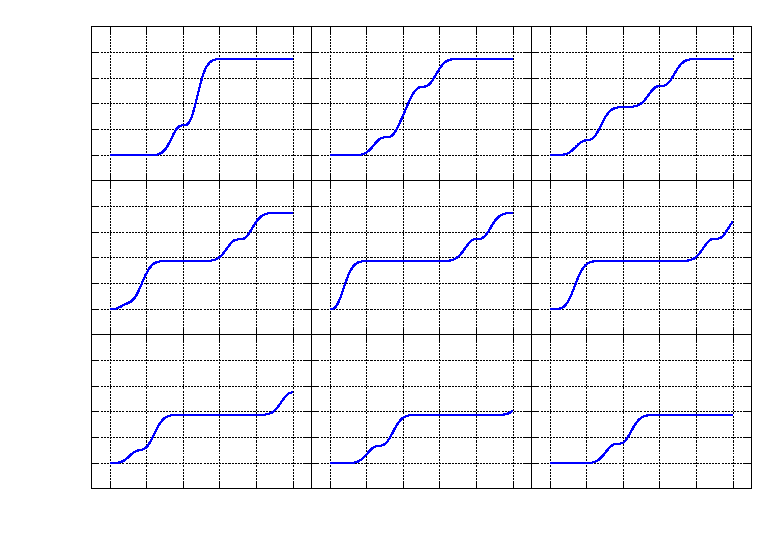
\includegraphics{mass_weak}}%
    \gplfronttext
  \end{picture}%
\endgroup

  \caption[Weak field results for the mass-aspect function $M(t,r)$.]{Weak field results for the mass-aspect function $M(t,r)$. The parameters of the run are $\eta=0.05$, $r_{0}=0$, $\delta=1$, $r_{\max}=64$, $w=0.15$, and $N_{r}=640$.}
  \label{fig:mass_weak}
\end{figure}

The strong field regime is obtained by choosing a value of $\eta$ which is larger than the critical value $\eta_{*}$, and is characterized by the gravitational collapse of the scalar field which leads to black hole formation. For the results presented in figures~\ref{fig:phi_strong},~\ref{fig:alpha_strong}, and~\ref{fig:mass_strong} we have set $\eta=0.6$. After a black hole forms, the code eventually crashes. The better the region around the black hole horizon, which can be determined by checking where $\frac{2M}{r}\approx1$, is resolved, the longer it will take for the code to crash, and the better we can estimiate the mass of the black hole and the horizon position. Our resolution was just high enough to keep to simulation from crashing immediately after black hole formation, but certainly our grid choice was not the best to resolve the horizon, as our grid is more densily sampled around $r\approx0$, not around $r\approx r_{\rm horizon}$.

The lapse function goes to zero\footnote{In the actual code the lapse reaches a very small value, below $10^{-3}$ for example, which is enough for us to characterize black hole formation.} in this regime, which tells us that around that region there is virtually no proper time being elapsed between one hypersurface of constant time and the next. This is known as the \emph{freezing of the lapse function}, and is a very useful feature to detect black hole formation.

Figure~\ref{fig:phi_strong} shows clearly that no time is passing for the scalar field after it collapses, since its evolution gets frozen. The freezing of the lapse function is evident in figure~\ref{fig:alpha_strong}, while the mass of the black hole formed (in code units) can be seen as the plateau of the function $M(t,r)$ in figure~\ref{fig:mass_strong}, and its value is $M_{\rm BH}\approx0.473$.

\begin{figure}[H]
  \centering
  % GNUPLOT: LaTeX picture with Postscript
\begingroup
  \makeatletter
  \providecommand\color[2][]{%
    \GenericError{(gnuplot) \space\space\space\@spaces}{%
      Package color not loaded in conjunction with
      terminal option `colourtext'%
    }{See the gnuplot documentation for explanation.%
    }{Either use 'blacktext' in gnuplot or load the package
      color.sty in LaTeX.}%
    \renewcommand\color[2][]{}%
  }%
  \providecommand\includegraphics[2][]{%
    \GenericError{(gnuplot) \space\space\space\@spaces}{%
      Package graphicx or graphics not loaded%
    }{See the gnuplot documentation for explanation.%
    }{The gnuplot epslatex terminal needs graphicx.sty or graphics.sty.}%
    \renewcommand\includegraphics[2][]{}%
  }%
  \providecommand\rotatebox[2]{#2}%
  \@ifundefined{ifGPcolor}{%
    \newif\ifGPcolor
    \GPcolorfalse
  }{}%
  \@ifundefined{ifGPblacktext}{%
    \newif\ifGPblacktext
    \GPblacktexttrue
  }{}%
  % define a \g@addto@macro without @ in the name:
  \let\gplgaddtomacro\g@addto@macro
  % define empty templates for all commands taking text:
  \gdef\gplbacktext{}%
  \gdef\gplfronttext{}%
  \makeatother
  \ifGPblacktext
    % no textcolor at all
    \def\colorrgb#1{}%
    \def\colorgray#1{}%
  \else
    % gray or color?
    \ifGPcolor
      \def\colorrgb#1{\color[rgb]{#1}}%
      \def\colorgray#1{\color[gray]{#1}}%
      \expandafter\def\csname LTw\endcsname{\color{white}}%
      \expandafter\def\csname LTb\endcsname{\color{black}}%
      \expandafter\def\csname LTa\endcsname{\color{black}}%
      \expandafter\def\csname LT0\endcsname{\color[rgb]{1,0,0}}%
      \expandafter\def\csname LT1\endcsname{\color[rgb]{0,1,0}}%
      \expandafter\def\csname LT2\endcsname{\color[rgb]{0,0,1}}%
      \expandafter\def\csname LT3\endcsname{\color[rgb]{1,0,1}}%
      \expandafter\def\csname LT4\endcsname{\color[rgb]{0,1,1}}%
      \expandafter\def\csname LT5\endcsname{\color[rgb]{1,1,0}}%
      \expandafter\def\csname LT6\endcsname{\color[rgb]{0,0,0}}%
      \expandafter\def\csname LT7\endcsname{\color[rgb]{1,0.3,0}}%
      \expandafter\def\csname LT8\endcsname{\color[rgb]{0.5,0.5,0.5}}%
    \else
      % gray
      \def\colorrgb#1{\color{black}}%
      \def\colorgray#1{\color[gray]{#1}}%
      \expandafter\def\csname LTw\endcsname{\color{white}}%
      \expandafter\def\csname LTb\endcsname{\color{black}}%
      \expandafter\def\csname LTa\endcsname{\color{black}}%
      \expandafter\def\csname LT0\endcsname{\color{black}}%
      \expandafter\def\csname LT1\endcsname{\color{black}}%
      \expandafter\def\csname LT2\endcsname{\color{black}}%
      \expandafter\def\csname LT3\endcsname{\color{black}}%
      \expandafter\def\csname LT4\endcsname{\color{black}}%
      \expandafter\def\csname LT5\endcsname{\color{black}}%
      \expandafter\def\csname LT6\endcsname{\color{black}}%
      \expandafter\def\csname LT7\endcsname{\color{black}}%
      \expandafter\def\csname LT8\endcsname{\color{black}}%
    \fi
  \fi
    \setlength{\unitlength}{0.0500bp}%
    \ifx\gptboxheight\undefined%
      \newlength{\gptboxheight}%
      \newlength{\gptboxwidth}%
      \newsavebox{\gptboxtext}%
    \fi%
    \setlength{\fboxrule}{0.5pt}%
    \setlength{\fboxsep}{1pt}%
\begin{picture}(7200.00,5040.00)%
    \gplgaddtomacro\gplbacktext{%
      \csname LTb\endcsname%%
      \put(588,3706){\makebox(0,0)[r]{\strut{}0.00}}%
      \csname LTb\endcsname%%
      \put(588,3953){\makebox(0,0)[r]{\strut{}0.15}}%
      \csname LTb\endcsname%%
      \put(588,4199){\makebox(0,0)[r]{\strut{}0.30}}%
      \csname LTb\endcsname%%
      \put(588,4445){\makebox(0,0)[r]{\strut{}0.45}}%
      \csname LTb\endcsname%%
      \put(588,4692){\makebox(0,0)[r]{\strut{}0.60}}%
      \csname LTb\endcsname%%
      \put(1072,3240){\makebox(0,0){\strut{}}}%
      \csname LTb\endcsname%%
      \put(1424,3240){\makebox(0,0){\strut{}}}%
      \csname LTb\endcsname%%
      \put(1776,3240){\makebox(0,0){\strut{}}}%
      \csname LTb\endcsname%%
      \put(2127,3240){\makebox(0,0){\strut{}}}%
      \csname LTb\endcsname%%
      \put(2479,3240){\makebox(0,0){\strut{}}}%
      \put(1776,4774){\makebox(0,0){\strut{}$t = 0.00$}}%
    }%
    \gplgaddtomacro\gplfronttext{%
      \csname LTb\endcsname%%
      \put(-50,4199){\rotatebox{-270}{\makebox(0,0){\strut{}$\phi(t,r)$}}}%
    }%
    \gplgaddtomacro\gplbacktext{%
      \csname LTb\endcsname%%
      \put(2700,3706){\makebox(0,0)[r]{\strut{}}}%
      \csname LTb\endcsname%%
      \put(2700,3953){\makebox(0,0)[r]{\strut{}}}%
      \csname LTb\endcsname%%
      \put(2700,4199){\makebox(0,0)[r]{\strut{}}}%
      \csname LTb\endcsname%%
      \put(2700,4445){\makebox(0,0)[r]{\strut{}}}%
      \csname LTb\endcsname%%
      \put(2700,4692){\makebox(0,0)[r]{\strut{}}}%
      \csname LTb\endcsname%%
      \put(3184,3240){\makebox(0,0){\strut{}}}%
      \csname LTb\endcsname%%
      \put(3536,3240){\makebox(0,0){\strut{}}}%
      \csname LTb\endcsname%%
      \put(3888,3240){\makebox(0,0){\strut{}}}%
      \csname LTb\endcsname%%
      \put(4239,3240){\makebox(0,0){\strut{}}}%
      \csname LTb\endcsname%%
      \put(4591,3240){\makebox(0,0){\strut{}}}%
      \put(3888,4774){\makebox(0,0){\strut{}$t = 1.27$}}%
    }%
    \gplgaddtomacro\gplfronttext{%
    }%
    \gplgaddtomacro\gplbacktext{%
      \csname LTb\endcsname%%
      \put(4812,3706){\makebox(0,0)[r]{\strut{}}}%
      \csname LTb\endcsname%%
      \put(4812,3953){\makebox(0,0)[r]{\strut{}}}%
      \csname LTb\endcsname%%
      \put(4812,4199){\makebox(0,0)[r]{\strut{}}}%
      \csname LTb\endcsname%%
      \put(4812,4445){\makebox(0,0)[r]{\strut{}}}%
      \csname LTb\endcsname%%
      \put(4812,4692){\makebox(0,0)[r]{\strut{}}}%
      \csname LTb\endcsname%%
      \put(5296,3240){\makebox(0,0){\strut{}}}%
      \csname LTb\endcsname%%
      \put(5648,3240){\makebox(0,0){\strut{}}}%
      \csname LTb\endcsname%%
      \put(6000,3240){\makebox(0,0){\strut{}}}%
      \csname LTb\endcsname%%
      \put(6351,3240){\makebox(0,0){\strut{}}}%
      \csname LTb\endcsname%%
      \put(6703,3240){\makebox(0,0){\strut{}}}%
      \put(6000,4774){\makebox(0,0){\strut{}$t = 2.55$}}%
    }%
    \gplgaddtomacro\gplfronttext{%
    }%
    \gplgaddtomacro\gplbacktext{%
      \csname LTb\endcsname%%
      \put(588,2228){\makebox(0,0)[r]{\strut{}0.00}}%
      \csname LTb\endcsname%%
      \put(588,2475){\makebox(0,0)[r]{\strut{}0.15}}%
      \csname LTb\endcsname%%
      \put(588,2721){\makebox(0,0)[r]{\strut{}0.30}}%
      \csname LTb\endcsname%%
      \put(588,2967){\makebox(0,0)[r]{\strut{}0.45}}%
      \csname LTb\endcsname%%
      \put(588,3214){\makebox(0,0)[r]{\strut{}0.60}}%
      \csname LTb\endcsname%%
      \put(1072,1762){\makebox(0,0){\strut{}}}%
      \csname LTb\endcsname%%
      \put(1424,1762){\makebox(0,0){\strut{}}}%
      \csname LTb\endcsname%%
      \put(1776,1762){\makebox(0,0){\strut{}}}%
      \csname LTb\endcsname%%
      \put(2127,1762){\makebox(0,0){\strut{}}}%
      \csname LTb\endcsname%%
      \put(2479,1762){\makebox(0,0){\strut{}}}%
      \put(1776,3296){\makebox(0,0){\strut{}$t = 3.82$}}%
    }%
    \gplgaddtomacro\gplfronttext{%
      \csname LTb\endcsname%%
      \put(-50,2721){\rotatebox{-270}{\makebox(0,0){\strut{}$\phi(t,r)$}}}%
    }%
    \gplgaddtomacro\gplbacktext{%
      \csname LTb\endcsname%%
      \put(2700,2228){\makebox(0,0)[r]{\strut{}}}%
      \csname LTb\endcsname%%
      \put(2700,2475){\makebox(0,0)[r]{\strut{}}}%
      \csname LTb\endcsname%%
      \put(2700,2721){\makebox(0,0)[r]{\strut{}}}%
      \csname LTb\endcsname%%
      \put(2700,2967){\makebox(0,0)[r]{\strut{}}}%
      \csname LTb\endcsname%%
      \put(2700,3214){\makebox(0,0)[r]{\strut{}}}%
      \csname LTb\endcsname%%
      \put(3184,1762){\makebox(0,0){\strut{}}}%
      \csname LTb\endcsname%%
      \put(3536,1762){\makebox(0,0){\strut{}}}%
      \csname LTb\endcsname%%
      \put(3888,1762){\makebox(0,0){\strut{}}}%
      \csname LTb\endcsname%%
      \put(4239,1762){\makebox(0,0){\strut{}}}%
      \csname LTb\endcsname%%
      \put(4591,1762){\makebox(0,0){\strut{}}}%
      \put(3888,3296){\makebox(0,0){\strut{}$t = 5.09$}}%
    }%
    \gplgaddtomacro\gplfronttext{%
    }%
    \gplgaddtomacro\gplbacktext{%
      \csname LTb\endcsname%%
      \put(4812,2228){\makebox(0,0)[r]{\strut{}}}%
      \csname LTb\endcsname%%
      \put(4812,2475){\makebox(0,0)[r]{\strut{}}}%
      \csname LTb\endcsname%%
      \put(4812,2721){\makebox(0,0)[r]{\strut{}}}%
      \csname LTb\endcsname%%
      \put(4812,2967){\makebox(0,0)[r]{\strut{}}}%
      \csname LTb\endcsname%%
      \put(4812,3214){\makebox(0,0)[r]{\strut{}}}%
      \csname LTb\endcsname%%
      \put(5296,1762){\makebox(0,0){\strut{}}}%
      \csname LTb\endcsname%%
      \put(5648,1762){\makebox(0,0){\strut{}}}%
      \csname LTb\endcsname%%
      \put(6000,1762){\makebox(0,0){\strut{}}}%
      \csname LTb\endcsname%%
      \put(6351,1762){\makebox(0,0){\strut{}}}%
      \csname LTb\endcsname%%
      \put(6703,1762){\makebox(0,0){\strut{}}}%
      \put(6000,3296){\makebox(0,0){\strut{}$t = 6.36$}}%
    }%
    \gplgaddtomacro\gplfronttext{%
    }%
    \gplgaddtomacro\gplbacktext{%
      \csname LTb\endcsname%%
      \put(588,750){\makebox(0,0)[r]{\strut{}0.00}}%
      \csname LTb\endcsname%%
      \put(588,997){\makebox(0,0)[r]{\strut{}0.15}}%
      \csname LTb\endcsname%%
      \put(588,1243){\makebox(0,0)[r]{\strut{}0.30}}%
      \csname LTb\endcsname%%
      \put(588,1489){\makebox(0,0)[r]{\strut{}0.45}}%
      \csname LTb\endcsname%%
      \put(588,1736){\makebox(0,0)[r]{\strut{}0.60}}%
      \csname LTb\endcsname%%
      \put(1072,284){\makebox(0,0){\strut{}$0$}}%
      \csname LTb\endcsname%%
      \put(1424,284){\makebox(0,0){\strut{}$1$}}%
      \csname LTb\endcsname%%
      \put(1776,284){\makebox(0,0){\strut{}$2$}}%
      \csname LTb\endcsname%%
      \put(2127,284){\makebox(0,0){\strut{}$3$}}%
      \csname LTb\endcsname%%
      \put(2479,284){\makebox(0,0){\strut{}$4$}}%
      \put(1776,1818){\makebox(0,0){\strut{}$t = 7.64$}}%
    }%
    \gplgaddtomacro\gplfronttext{%
      \csname LTb\endcsname%%
      \put(-50,1243){\rotatebox{-270}{\makebox(0,0){\strut{}$\phi(t,r)$}}}%
      \put(1775,-46){\makebox(0,0){\strut{}$r$}}%
    }%
    \gplgaddtomacro\gplbacktext{%
      \csname LTb\endcsname%%
      \put(2700,750){\makebox(0,0)[r]{\strut{}}}%
      \csname LTb\endcsname%%
      \put(2700,997){\makebox(0,0)[r]{\strut{}}}%
      \csname LTb\endcsname%%
      \put(2700,1243){\makebox(0,0)[r]{\strut{}}}%
      \csname LTb\endcsname%%
      \put(2700,1489){\makebox(0,0)[r]{\strut{}}}%
      \csname LTb\endcsname%%
      \put(2700,1736){\makebox(0,0)[r]{\strut{}}}%
      \csname LTb\endcsname%%
      \put(3184,284){\makebox(0,0){\strut{}$0$}}%
      \csname LTb\endcsname%%
      \put(3536,284){\makebox(0,0){\strut{}$1$}}%
      \csname LTb\endcsname%%
      \put(3888,284){\makebox(0,0){\strut{}$2$}}%
      \csname LTb\endcsname%%
      \put(4239,284){\makebox(0,0){\strut{}$3$}}%
      \csname LTb\endcsname%%
      \put(4591,284){\makebox(0,0){\strut{}$4$}}%
      \put(3888,1818){\makebox(0,0){\strut{}$t = 8.91$}}%
    }%
    \gplgaddtomacro\gplfronttext{%
      \csname LTb\endcsname%%
      \put(3887,-46){\makebox(0,0){\strut{}$r$}}%
    }%
    \gplgaddtomacro\gplbacktext{%
      \csname LTb\endcsname%%
      \put(4812,750){\makebox(0,0)[r]{\strut{}}}%
      \csname LTb\endcsname%%
      \put(4812,997){\makebox(0,0)[r]{\strut{}}}%
      \csname LTb\endcsname%%
      \put(4812,1243){\makebox(0,0)[r]{\strut{}}}%
      \csname LTb\endcsname%%
      \put(4812,1489){\makebox(0,0)[r]{\strut{}}}%
      \csname LTb\endcsname%%
      \put(4812,1736){\makebox(0,0)[r]{\strut{}}}%
      \csname LTb\endcsname%%
      \put(5296,284){\makebox(0,0){\strut{}$0$}}%
      \csname LTb\endcsname%%
      \put(5648,284){\makebox(0,0){\strut{}$1$}}%
      \csname LTb\endcsname%%
      \put(6000,284){\makebox(0,0){\strut{}$2$}}%
      \csname LTb\endcsname%%
      \put(6351,284){\makebox(0,0){\strut{}$3$}}%
      \csname LTb\endcsname%%
      \put(6703,284){\makebox(0,0){\strut{}$4$}}%
      \put(6000,1818){\makebox(0,0){\strut{}$t = 10.18$}}%
    }%
    \gplgaddtomacro\gplfronttext{%
      \csname LTb\endcsname%%
      \put(5999,-46){\makebox(0,0){\strut{}$r$}}%
    }%
    \gplbacktext
    \put(0,0){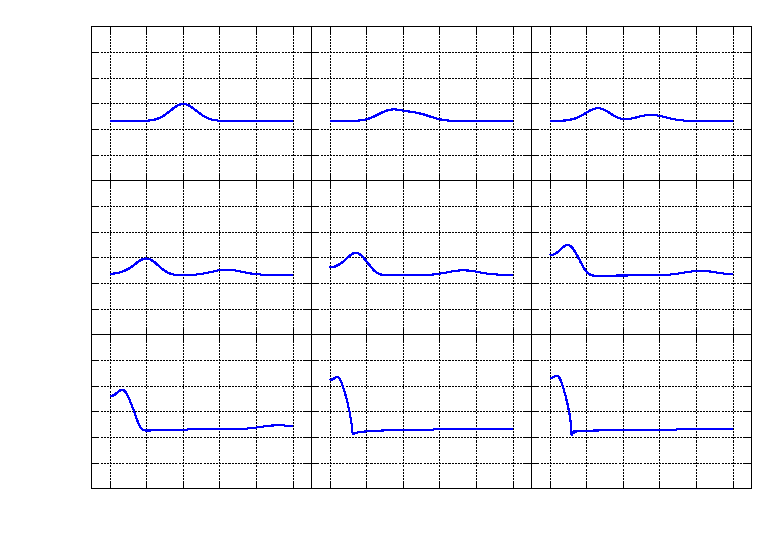
\includegraphics{resources/scalarfield_strong}}%
    \gplfronttext
  \end{picture}%
\endgroup

  \caption[Strong field results for the scalar field $\phi(t,r)$.]{Strong field results for the scalar field $\phi(t,r)$. The parameters of the run are $\eta=0.6$, $r_{0}=0$, $\delta=1$, $r_{\max}=64$, $w=0.15$, and $N_{r}=640$.}
  \label{fig:phi_strong}
\end{figure}

\begin{figure}[H]
  \centering
  % GNUPLOT: LaTeX picture with Postscript
\begingroup
  \makeatletter
  \providecommand\color[2][]{%
    \GenericError{(gnuplot) \space\space\space\@spaces}{%
      Package color not loaded in conjunction with
      terminal option `colourtext'%
    }{See the gnuplot documentation for explanation.%
    }{Either use 'blacktext' in gnuplot or load the package
      color.sty in LaTeX.}%
    \renewcommand\color[2][]{}%
  }%
  \providecommand\includegraphics[2][]{%
    \GenericError{(gnuplot) \space\space\space\@spaces}{%
      Package graphicx or graphics not loaded%
    }{See the gnuplot documentation for explanation.%
    }{The gnuplot epslatex terminal needs graphicx.sty or graphics.sty.}%
    \renewcommand\includegraphics[2][]{}%
  }%
  \providecommand\rotatebox[2]{#2}%
  \@ifundefined{ifGPcolor}{%
    \newif\ifGPcolor
    \GPcolorfalse
  }{}%
  \@ifundefined{ifGPblacktext}{%
    \newif\ifGPblacktext
    \GPblacktexttrue
  }{}%
  % define a \g@addto@macro without @ in the name:
  \let\gplgaddtomacro\g@addto@macro
  % define empty templates for all commands taking text:
  \gdef\gplbacktext{}%
  \gdef\gplfronttext{}%
  \makeatother
  \ifGPblacktext
    % no textcolor at all
    \def\colorrgb#1{}%
    \def\colorgray#1{}%
  \else
    % gray or color?
    \ifGPcolor
      \def\colorrgb#1{\color[rgb]{#1}}%
      \def\colorgray#1{\color[gray]{#1}}%
      \expandafter\def\csname LTw\endcsname{\color{white}}%
      \expandafter\def\csname LTb\endcsname{\color{black}}%
      \expandafter\def\csname LTa\endcsname{\color{black}}%
      \expandafter\def\csname LT0\endcsname{\color[rgb]{1,0,0}}%
      \expandafter\def\csname LT1\endcsname{\color[rgb]{0,1,0}}%
      \expandafter\def\csname LT2\endcsname{\color[rgb]{0,0,1}}%
      \expandafter\def\csname LT3\endcsname{\color[rgb]{1,0,1}}%
      \expandafter\def\csname LT4\endcsname{\color[rgb]{0,1,1}}%
      \expandafter\def\csname LT5\endcsname{\color[rgb]{1,1,0}}%
      \expandafter\def\csname LT6\endcsname{\color[rgb]{0,0,0}}%
      \expandafter\def\csname LT7\endcsname{\color[rgb]{1,0.3,0}}%
      \expandafter\def\csname LT8\endcsname{\color[rgb]{0.5,0.5,0.5}}%
    \else
      % gray
      \def\colorrgb#1{\color{black}}%
      \def\colorgray#1{\color[gray]{#1}}%
      \expandafter\def\csname LTw\endcsname{\color{white}}%
      \expandafter\def\csname LTb\endcsname{\color{black}}%
      \expandafter\def\csname LTa\endcsname{\color{black}}%
      \expandafter\def\csname LT0\endcsname{\color{black}}%
      \expandafter\def\csname LT1\endcsname{\color{black}}%
      \expandafter\def\csname LT2\endcsname{\color{black}}%
      \expandafter\def\csname LT3\endcsname{\color{black}}%
      \expandafter\def\csname LT4\endcsname{\color{black}}%
      \expandafter\def\csname LT5\endcsname{\color{black}}%
      \expandafter\def\csname LT6\endcsname{\color{black}}%
      \expandafter\def\csname LT7\endcsname{\color{black}}%
      \expandafter\def\csname LT8\endcsname{\color{black}}%
    \fi
  \fi
    \setlength{\unitlength}{0.0500bp}%
    \ifx\gptboxheight\undefined%
      \newlength{\gptboxheight}%
      \newlength{\gptboxwidth}%
      \newsavebox{\gptboxtext}%
    \fi%
    \setlength{\fboxrule}{0.5pt}%
    \setlength{\fboxsep}{1pt}%
\begin{picture}(7200.00,5040.00)%
    \gplgaddtomacro\gplbacktext{%
      \csname LTb\endcsname%%
      \put(588,3706){\makebox(0,0)[r]{\strut{}0.0}}%
      \csname LTb\endcsname%%
      \put(588,3953){\makebox(0,0)[r]{\strut{}0.3}}%
      \csname LTb\endcsname%%
      \put(588,4199){\makebox(0,0)[r]{\strut{}0.6}}%
      \csname LTb\endcsname%%
      \put(588,4445){\makebox(0,0)[r]{\strut{}0.9}}%
      \csname LTb\endcsname%%
      \put(588,4692){\makebox(0,0)[r]{\strut{}1.2}}%
      \csname LTb\endcsname%%
      \put(896,3240){\makebox(0,0){\strut{}}}%
      \csname LTb\endcsname%%
      \put(1248,3240){\makebox(0,0){\strut{}}}%
      \csname LTb\endcsname%%
      \put(1600,3240){\makebox(0,0){\strut{}}}%
      \csname LTb\endcsname%%
      \put(1951,3240){\makebox(0,0){\strut{}}}%
      \csname LTb\endcsname%%
      \put(2303,3240){\makebox(0,0){\strut{}}}%
      \csname LTb\endcsname%%
      \put(2655,3240){\makebox(0,0){\strut{}}}%
      \put(1776,4774){\makebox(0,0){\strut{}$t = 0$}}%
    }%
    \gplgaddtomacro\gplfronttext{%
      \csname LTb\endcsname%%
      \put(82,4199){\rotatebox{-270}{\makebox(0,0){\strut{}$\alpha(t,r)$}}}%
    }%
    \gplgaddtomacro\gplbacktext{%
      \csname LTb\endcsname%%
      \put(2700,3706){\makebox(0,0)[r]{\strut{}}}%
      \csname LTb\endcsname%%
      \put(2700,3953){\makebox(0,0)[r]{\strut{}}}%
      \csname LTb\endcsname%%
      \put(2700,4199){\makebox(0,0)[r]{\strut{}}}%
      \csname LTb\endcsname%%
      \put(2700,4445){\makebox(0,0)[r]{\strut{}}}%
      \csname LTb\endcsname%%
      \put(2700,4692){\makebox(0,0)[r]{\strut{}}}%
      \csname LTb\endcsname%%
      \put(3008,3240){\makebox(0,0){\strut{}}}%
      \csname LTb\endcsname%%
      \put(3360,3240){\makebox(0,0){\strut{}}}%
      \csname LTb\endcsname%%
      \put(3712,3240){\makebox(0,0){\strut{}}}%
      \csname LTb\endcsname%%
      \put(4063,3240){\makebox(0,0){\strut{}}}%
      \csname LTb\endcsname%%
      \put(4415,3240){\makebox(0,0){\strut{}}}%
      \csname LTb\endcsname%%
      \put(4767,3240){\makebox(0,0){\strut{}}}%
      \put(3888,4774){\makebox(0,0){\strut{}$t = 0.5\times10^{3}\Delta t$}}%
    }%
    \gplgaddtomacro\gplfronttext{%
    }%
    \gplgaddtomacro\gplbacktext{%
      \csname LTb\endcsname%%
      \put(4812,3706){\makebox(0,0)[r]{\strut{}}}%
      \csname LTb\endcsname%%
      \put(4812,3953){\makebox(0,0)[r]{\strut{}}}%
      \csname LTb\endcsname%%
      \put(4812,4199){\makebox(0,0)[r]{\strut{}}}%
      \csname LTb\endcsname%%
      \put(4812,4445){\makebox(0,0)[r]{\strut{}}}%
      \csname LTb\endcsname%%
      \put(4812,4692){\makebox(0,0)[r]{\strut{}}}%
      \csname LTb\endcsname%%
      \put(5120,3240){\makebox(0,0){\strut{}}}%
      \csname LTb\endcsname%%
      \put(5472,3240){\makebox(0,0){\strut{}}}%
      \csname LTb\endcsname%%
      \put(5824,3240){\makebox(0,0){\strut{}}}%
      \csname LTb\endcsname%%
      \put(6175,3240){\makebox(0,0){\strut{}}}%
      \csname LTb\endcsname%%
      \put(6527,3240){\makebox(0,0){\strut{}}}%
      \csname LTb\endcsname%%
      \put(6879,3240){\makebox(0,0){\strut{}}}%
      \put(6000,4774){\makebox(0,0){\strut{}$t = 1.0\times10^{3}\Delta t$}}%
    }%
    \gplgaddtomacro\gplfronttext{%
    }%
    \gplgaddtomacro\gplbacktext{%
      \csname LTb\endcsname%%
      \put(588,2228){\makebox(0,0)[r]{\strut{}0.0}}%
      \csname LTb\endcsname%%
      \put(588,2475){\makebox(0,0)[r]{\strut{}0.3}}%
      \csname LTb\endcsname%%
      \put(588,2721){\makebox(0,0)[r]{\strut{}0.6}}%
      \csname LTb\endcsname%%
      \put(588,2967){\makebox(0,0)[r]{\strut{}0.9}}%
      \csname LTb\endcsname%%
      \put(588,3214){\makebox(0,0)[r]{\strut{}1.2}}%
      \csname LTb\endcsname%%
      \put(896,1762){\makebox(0,0){\strut{}}}%
      \csname LTb\endcsname%%
      \put(1248,1762){\makebox(0,0){\strut{}}}%
      \csname LTb\endcsname%%
      \put(1600,1762){\makebox(0,0){\strut{}}}%
      \csname LTb\endcsname%%
      \put(1951,1762){\makebox(0,0){\strut{}}}%
      \csname LTb\endcsname%%
      \put(2303,1762){\makebox(0,0){\strut{}}}%
      \csname LTb\endcsname%%
      \put(2655,1762){\makebox(0,0){\strut{}}}%
      \put(1776,3296){\makebox(0,0){\strut{}$t = 1.5\times10^{3}\Delta t$}}%
    }%
    \gplgaddtomacro\gplfronttext{%
      \csname LTb\endcsname%%
      \put(82,2721){\rotatebox{-270}{\makebox(0,0){\strut{}$\alpha(t,r)$}}}%
    }%
    \gplgaddtomacro\gplbacktext{%
      \csname LTb\endcsname%%
      \put(2700,2228){\makebox(0,0)[r]{\strut{}}}%
      \csname LTb\endcsname%%
      \put(2700,2475){\makebox(0,0)[r]{\strut{}}}%
      \csname LTb\endcsname%%
      \put(2700,2721){\makebox(0,0)[r]{\strut{}}}%
      \csname LTb\endcsname%%
      \put(2700,2967){\makebox(0,0)[r]{\strut{}}}%
      \csname LTb\endcsname%%
      \put(2700,3214){\makebox(0,0)[r]{\strut{}}}%
      \csname LTb\endcsname%%
      \put(3008,1762){\makebox(0,0){\strut{}}}%
      \csname LTb\endcsname%%
      \put(3360,1762){\makebox(0,0){\strut{}}}%
      \csname LTb\endcsname%%
      \put(3712,1762){\makebox(0,0){\strut{}}}%
      \csname LTb\endcsname%%
      \put(4063,1762){\makebox(0,0){\strut{}}}%
      \csname LTb\endcsname%%
      \put(4415,1762){\makebox(0,0){\strut{}}}%
      \csname LTb\endcsname%%
      \put(4767,1762){\makebox(0,0){\strut{}}}%
      \put(3888,3296){\makebox(0,0){\strut{}$t = 2.0\times10^{3}\Delta t$}}%
    }%
    \gplgaddtomacro\gplfronttext{%
    }%
    \gplgaddtomacro\gplbacktext{%
      \csname LTb\endcsname%%
      \put(4812,2228){\makebox(0,0)[r]{\strut{}}}%
      \csname LTb\endcsname%%
      \put(4812,2475){\makebox(0,0)[r]{\strut{}}}%
      \csname LTb\endcsname%%
      \put(4812,2721){\makebox(0,0)[r]{\strut{}}}%
      \csname LTb\endcsname%%
      \put(4812,2967){\makebox(0,0)[r]{\strut{}}}%
      \csname LTb\endcsname%%
      \put(4812,3214){\makebox(0,0)[r]{\strut{}}}%
      \csname LTb\endcsname%%
      \put(5120,1762){\makebox(0,0){\strut{}}}%
      \csname LTb\endcsname%%
      \put(5472,1762){\makebox(0,0){\strut{}}}%
      \csname LTb\endcsname%%
      \put(5824,1762){\makebox(0,0){\strut{}}}%
      \csname LTb\endcsname%%
      \put(6175,1762){\makebox(0,0){\strut{}}}%
      \csname LTb\endcsname%%
      \put(6527,1762){\makebox(0,0){\strut{}}}%
      \csname LTb\endcsname%%
      \put(6879,1762){\makebox(0,0){\strut{}}}%
      \put(6000,3296){\makebox(0,0){\strut{}$t = 2.5\times10^{3}\Delta t$}}%
    }%
    \gplgaddtomacro\gplfronttext{%
    }%
    \gplgaddtomacro\gplbacktext{%
      \csname LTb\endcsname%%
      \put(588,750){\makebox(0,0)[r]{\strut{}0.0}}%
      \csname LTb\endcsname%%
      \put(588,997){\makebox(0,0)[r]{\strut{}0.3}}%
      \csname LTb\endcsname%%
      \put(588,1243){\makebox(0,0)[r]{\strut{}0.6}}%
      \csname LTb\endcsname%%
      \put(588,1489){\makebox(0,0)[r]{\strut{}0.9}}%
      \csname LTb\endcsname%%
      \put(588,1736){\makebox(0,0)[r]{\strut{}1.2}}%
      \csname LTb\endcsname%%
      \put(896,284){\makebox(0,0){\strut{}$0$}}%
      \csname LTb\endcsname%%
      \put(1248,284){\makebox(0,0){\strut{}$10$}}%
      \csname LTb\endcsname%%
      \put(1600,284){\makebox(0,0){\strut{}$20$}}%
      \csname LTb\endcsname%%
      \put(1951,284){\makebox(0,0){\strut{}$30$}}%
      \csname LTb\endcsname%%
      \put(2303,284){\makebox(0,0){\strut{}$40$}}%
      \csname LTb\endcsname%%
      \put(2655,284){\makebox(0,0){\strut{}$50$}}%
      \put(1776,1818){\makebox(0,0){\strut{}$t = 3.0\times10^{3}\Delta t$}}%
    }%
    \gplgaddtomacro\gplfronttext{%
      \csname LTb\endcsname%%
      \put(82,1243){\rotatebox{-270}{\makebox(0,0){\strut{}$\alpha(t,r)$}}}%
      \put(1775,-46){\makebox(0,0){\strut{}$r$}}%
    }%
    \gplgaddtomacro\gplbacktext{%
      \csname LTb\endcsname%%
      \put(2700,750){\makebox(0,0)[r]{\strut{}}}%
      \csname LTb\endcsname%%
      \put(2700,997){\makebox(0,0)[r]{\strut{}}}%
      \csname LTb\endcsname%%
      \put(2700,1243){\makebox(0,0)[r]{\strut{}}}%
      \csname LTb\endcsname%%
      \put(2700,1489){\makebox(0,0)[r]{\strut{}}}%
      \csname LTb\endcsname%%
      \put(2700,1736){\makebox(0,0)[r]{\strut{}}}%
      \csname LTb\endcsname%%
      \put(3008,284){\makebox(0,0){\strut{}$0$}}%
      \csname LTb\endcsname%%
      \put(3360,284){\makebox(0,0){\strut{}$10$}}%
      \csname LTb\endcsname%%
      \put(3712,284){\makebox(0,0){\strut{}$20$}}%
      \csname LTb\endcsname%%
      \put(4063,284){\makebox(0,0){\strut{}$30$}}%
      \csname LTb\endcsname%%
      \put(4415,284){\makebox(0,0){\strut{}$40$}}%
      \csname LTb\endcsname%%
      \put(4767,284){\makebox(0,0){\strut{}$50$}}%
      \put(3888,1818){\makebox(0,0){\strut{}$t = 4.5\times10^{3}\Delta t$}}%
    }%
    \gplgaddtomacro\gplfronttext{%
      \csname LTb\endcsname%%
      \put(3887,-46){\makebox(0,0){\strut{}$r$}}%
    }%
    \gplgaddtomacro\gplbacktext{%
      \csname LTb\endcsname%%
      \put(4812,750){\makebox(0,0)[r]{\strut{}}}%
      \csname LTb\endcsname%%
      \put(4812,997){\makebox(0,0)[r]{\strut{}}}%
      \csname LTb\endcsname%%
      \put(4812,1243){\makebox(0,0)[r]{\strut{}}}%
      \csname LTb\endcsname%%
      \put(4812,1489){\makebox(0,0)[r]{\strut{}}}%
      \csname LTb\endcsname%%
      \put(4812,1736){\makebox(0,0)[r]{\strut{}}}%
      \csname LTb\endcsname%%
      \put(5120,284){\makebox(0,0){\strut{}$0$}}%
      \csname LTb\endcsname%%
      \put(5472,284){\makebox(0,0){\strut{}$10$}}%
      \csname LTb\endcsname%%
      \put(5824,284){\makebox(0,0){\strut{}$20$}}%
      \csname LTb\endcsname%%
      \put(6175,284){\makebox(0,0){\strut{}$30$}}%
      \csname LTb\endcsname%%
      \put(6527,284){\makebox(0,0){\strut{}$40$}}%
      \csname LTb\endcsname%%
      \put(6879,284){\makebox(0,0){\strut{}$50$}}%
      \put(6000,1818){\makebox(0,0){\strut{}$t = 6.0\times10^{3}\Delta t$}}%
    }%
    \gplgaddtomacro\gplfronttext{%
      \csname LTb\endcsname%%
      \put(5999,-46){\makebox(0,0){\strut{}$r$}}%
    }%
    \gplbacktext
    \put(0,0){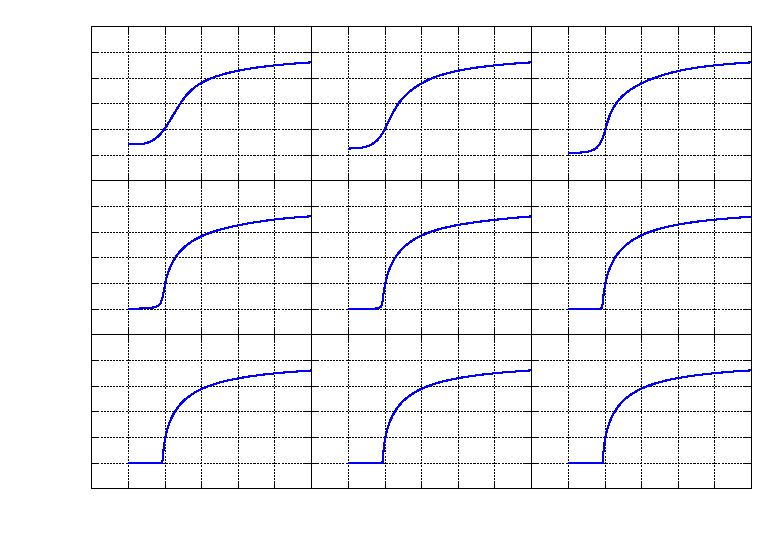
\includegraphics{alpha_strong}}%
    \gplfronttext
  \end{picture}%
\endgroup

  \caption[Strong field results for the lapse function $\a(t,r)$.]{Strong field results for the lapse function $\a(t,r)$. The parameters of the run are $\eta=0.6$, $r_{0}=0$, $\delta=1$, $r_{\max}=64$, $w=0.15$, and $N_{r}=640$.}
  \label{fig:alpha_strong}
\end{figure}

\begin{figure}[H]
  \centering
  % GNUPLOT: LaTeX picture with Postscript
\begingroup
  \makeatletter
  \providecommand\color[2][]{%
    \GenericError{(gnuplot) \space\space\space\@spaces}{%
      Package color not loaded in conjunction with
      terminal option `colourtext'%
    }{See the gnuplot documentation for explanation.%
    }{Either use 'blacktext' in gnuplot or load the package
      color.sty in LaTeX.}%
    \renewcommand\color[2][]{}%
  }%
  \providecommand\includegraphics[2][]{%
    \GenericError{(gnuplot) \space\space\space\@spaces}{%
      Package graphicx or graphics not loaded%
    }{See the gnuplot documentation for explanation.%
    }{The gnuplot epslatex terminal needs graphicx.sty or graphics.sty.}%
    \renewcommand\includegraphics[2][]{}%
  }%
  \providecommand\rotatebox[2]{#2}%
  \@ifundefined{ifGPcolor}{%
    \newif\ifGPcolor
    \GPcolorfalse
  }{}%
  \@ifundefined{ifGPblacktext}{%
    \newif\ifGPblacktext
    \GPblacktexttrue
  }{}%
  % define a \g@addto@macro without @ in the name:
  \let\gplgaddtomacro\g@addto@macro
  % define empty templates for all commands taking text:
  \gdef\gplbacktext{}%
  \gdef\gplfronttext{}%
  \makeatother
  \ifGPblacktext
    % no textcolor at all
    \def\colorrgb#1{}%
    \def\colorgray#1{}%
  \else
    % gray or color?
    \ifGPcolor
      \def\colorrgb#1{\color[rgb]{#1}}%
      \def\colorgray#1{\color[gray]{#1}}%
      \expandafter\def\csname LTw\endcsname{\color{white}}%
      \expandafter\def\csname LTb\endcsname{\color{black}}%
      \expandafter\def\csname LTa\endcsname{\color{black}}%
      \expandafter\def\csname LT0\endcsname{\color[rgb]{1,0,0}}%
      \expandafter\def\csname LT1\endcsname{\color[rgb]{0,1,0}}%
      \expandafter\def\csname LT2\endcsname{\color[rgb]{0,0,1}}%
      \expandafter\def\csname LT3\endcsname{\color[rgb]{1,0,1}}%
      \expandafter\def\csname LT4\endcsname{\color[rgb]{0,1,1}}%
      \expandafter\def\csname LT5\endcsname{\color[rgb]{1,1,0}}%
      \expandafter\def\csname LT6\endcsname{\color[rgb]{0,0,0}}%
      \expandafter\def\csname LT7\endcsname{\color[rgb]{1,0.3,0}}%
      \expandafter\def\csname LT8\endcsname{\color[rgb]{0.5,0.5,0.5}}%
    \else
      % gray
      \def\colorrgb#1{\color{black}}%
      \def\colorgray#1{\color[gray]{#1}}%
      \expandafter\def\csname LTw\endcsname{\color{white}}%
      \expandafter\def\csname LTb\endcsname{\color{black}}%
      \expandafter\def\csname LTa\endcsname{\color{black}}%
      \expandafter\def\csname LT0\endcsname{\color{black}}%
      \expandafter\def\csname LT1\endcsname{\color{black}}%
      \expandafter\def\csname LT2\endcsname{\color{black}}%
      \expandafter\def\csname LT3\endcsname{\color{black}}%
      \expandafter\def\csname LT4\endcsname{\color{black}}%
      \expandafter\def\csname LT5\endcsname{\color{black}}%
      \expandafter\def\csname LT6\endcsname{\color{black}}%
      \expandafter\def\csname LT7\endcsname{\color{black}}%
      \expandafter\def\csname LT8\endcsname{\color{black}}%
    \fi
  \fi
    \setlength{\unitlength}{0.0500bp}%
    \ifx\gptboxheight\undefined%
      \newlength{\gptboxheight}%
      \newlength{\gptboxwidth}%
      \newsavebox{\gptboxtext}%
    \fi%
    \setlength{\fboxrule}{0.5pt}%
    \setlength{\fboxsep}{1pt}%
\begin{picture}(7200.00,5040.00)%
    \gplgaddtomacro\gplbacktext{%
      \csname LTb\endcsname%%
      \put(588,3706){\makebox(0,0)[r]{\strut{}0.0}}%
      \csname LTb\endcsname%%
      \put(588,3953){\makebox(0,0)[r]{\strut{}1.5}}%
      \csname LTb\endcsname%%
      \put(588,4199){\makebox(0,0)[r]{\strut{}3.0}}%
      \csname LTb\endcsname%%
      \put(588,4445){\makebox(0,0)[r]{\strut{}4.5}}%
      \csname LTb\endcsname%%
      \put(588,4692){\makebox(0,0)[r]{\strut{}6.0}}%
      \csname LTb\endcsname%%
      \put(896,3240){\makebox(0,0){\strut{}}}%
      \csname LTb\endcsname%%
      \put(1248,3240){\makebox(0,0){\strut{}}}%
      \csname LTb\endcsname%%
      \put(1600,3240){\makebox(0,0){\strut{}}}%
      \csname LTb\endcsname%%
      \put(1951,3240){\makebox(0,0){\strut{}}}%
      \csname LTb\endcsname%%
      \put(2303,3240){\makebox(0,0){\strut{}}}%
      \csname LTb\endcsname%%
      \put(2655,3240){\makebox(0,0){\strut{}}}%
      \put(1776,4774){\makebox(0,0){\strut{}$t = 0$}}%
    }%
    \gplgaddtomacro\gplfronttext{%
      \csname LTb\endcsname%%
      \put(82,4199){\rotatebox{-270}{\makebox(0,0){\strut{}$M(t,r)$}}}%
    }%
    \gplgaddtomacro\gplbacktext{%
      \csname LTb\endcsname%%
      \put(2700,3706){\makebox(0,0)[r]{\strut{}}}%
      \csname LTb\endcsname%%
      \put(2700,3953){\makebox(0,0)[r]{\strut{}}}%
      \csname LTb\endcsname%%
      \put(2700,4199){\makebox(0,0)[r]{\strut{}}}%
      \csname LTb\endcsname%%
      \put(2700,4445){\makebox(0,0)[r]{\strut{}}}%
      \csname LTb\endcsname%%
      \put(2700,4692){\makebox(0,0)[r]{\strut{}}}%
      \csname LTb\endcsname%%
      \put(3008,3240){\makebox(0,0){\strut{}}}%
      \csname LTb\endcsname%%
      \put(3360,3240){\makebox(0,0){\strut{}}}%
      \csname LTb\endcsname%%
      \put(3712,3240){\makebox(0,0){\strut{}}}%
      \csname LTb\endcsname%%
      \put(4063,3240){\makebox(0,0){\strut{}}}%
      \csname LTb\endcsname%%
      \put(4415,3240){\makebox(0,0){\strut{}}}%
      \csname LTb\endcsname%%
      \put(4767,3240){\makebox(0,0){\strut{}}}%
      \put(3888,4774){\makebox(0,0){\strut{}$t = 0.5\times10^{3}\Delta t$}}%
    }%
    \gplgaddtomacro\gplfronttext{%
    }%
    \gplgaddtomacro\gplbacktext{%
      \csname LTb\endcsname%%
      \put(4812,3706){\makebox(0,0)[r]{\strut{}}}%
      \csname LTb\endcsname%%
      \put(4812,3953){\makebox(0,0)[r]{\strut{}}}%
      \csname LTb\endcsname%%
      \put(4812,4199){\makebox(0,0)[r]{\strut{}}}%
      \csname LTb\endcsname%%
      \put(4812,4445){\makebox(0,0)[r]{\strut{}}}%
      \csname LTb\endcsname%%
      \put(4812,4692){\makebox(0,0)[r]{\strut{}}}%
      \csname LTb\endcsname%%
      \put(5120,3240){\makebox(0,0){\strut{}}}%
      \csname LTb\endcsname%%
      \put(5472,3240){\makebox(0,0){\strut{}}}%
      \csname LTb\endcsname%%
      \put(5824,3240){\makebox(0,0){\strut{}}}%
      \csname LTb\endcsname%%
      \put(6175,3240){\makebox(0,0){\strut{}}}%
      \csname LTb\endcsname%%
      \put(6527,3240){\makebox(0,0){\strut{}}}%
      \csname LTb\endcsname%%
      \put(6879,3240){\makebox(0,0){\strut{}}}%
      \put(6000,4774){\makebox(0,0){\strut{}$t = 1.0\times10^{3}\Delta t$}}%
    }%
    \gplgaddtomacro\gplfronttext{%
    }%
    \gplgaddtomacro\gplbacktext{%
      \csname LTb\endcsname%%
      \put(588,2228){\makebox(0,0)[r]{\strut{}0.0}}%
      \csname LTb\endcsname%%
      \put(588,2475){\makebox(0,0)[r]{\strut{}1.5}}%
      \csname LTb\endcsname%%
      \put(588,2721){\makebox(0,0)[r]{\strut{}3.0}}%
      \csname LTb\endcsname%%
      \put(588,2967){\makebox(0,0)[r]{\strut{}4.5}}%
      \csname LTb\endcsname%%
      \put(588,3214){\makebox(0,0)[r]{\strut{}6.0}}%
      \csname LTb\endcsname%%
      \put(896,1762){\makebox(0,0){\strut{}}}%
      \csname LTb\endcsname%%
      \put(1248,1762){\makebox(0,0){\strut{}}}%
      \csname LTb\endcsname%%
      \put(1600,1762){\makebox(0,0){\strut{}}}%
      \csname LTb\endcsname%%
      \put(1951,1762){\makebox(0,0){\strut{}}}%
      \csname LTb\endcsname%%
      \put(2303,1762){\makebox(0,0){\strut{}}}%
      \csname LTb\endcsname%%
      \put(2655,1762){\makebox(0,0){\strut{}}}%
      \put(1776,3296){\makebox(0,0){\strut{}$t = 1.5\times10^{3}\Delta t$}}%
    }%
    \gplgaddtomacro\gplfronttext{%
      \csname LTb\endcsname%%
      \put(82,2721){\rotatebox{-270}{\makebox(0,0){\strut{}$M(t,r)$}}}%
    }%
    \gplgaddtomacro\gplbacktext{%
      \csname LTb\endcsname%%
      \put(2700,2228){\makebox(0,0)[r]{\strut{}}}%
      \csname LTb\endcsname%%
      \put(2700,2475){\makebox(0,0)[r]{\strut{}}}%
      \csname LTb\endcsname%%
      \put(2700,2721){\makebox(0,0)[r]{\strut{}}}%
      \csname LTb\endcsname%%
      \put(2700,2967){\makebox(0,0)[r]{\strut{}}}%
      \csname LTb\endcsname%%
      \put(2700,3214){\makebox(0,0)[r]{\strut{}}}%
      \csname LTb\endcsname%%
      \put(3008,1762){\makebox(0,0){\strut{}}}%
      \csname LTb\endcsname%%
      \put(3360,1762){\makebox(0,0){\strut{}}}%
      \csname LTb\endcsname%%
      \put(3712,1762){\makebox(0,0){\strut{}}}%
      \csname LTb\endcsname%%
      \put(4063,1762){\makebox(0,0){\strut{}}}%
      \csname LTb\endcsname%%
      \put(4415,1762){\makebox(0,0){\strut{}}}%
      \csname LTb\endcsname%%
      \put(4767,1762){\makebox(0,0){\strut{}}}%
      \put(3888,3296){\makebox(0,0){\strut{}$t = 2.0\times10^{3}\Delta t$}}%
    }%
    \gplgaddtomacro\gplfronttext{%
    }%
    \gplgaddtomacro\gplbacktext{%
      \csname LTb\endcsname%%
      \put(4812,2228){\makebox(0,0)[r]{\strut{}}}%
      \csname LTb\endcsname%%
      \put(4812,2475){\makebox(0,0)[r]{\strut{}}}%
      \csname LTb\endcsname%%
      \put(4812,2721){\makebox(0,0)[r]{\strut{}}}%
      \csname LTb\endcsname%%
      \put(4812,2967){\makebox(0,0)[r]{\strut{}}}%
      \csname LTb\endcsname%%
      \put(4812,3214){\makebox(0,0)[r]{\strut{}}}%
      \csname LTb\endcsname%%
      \put(5120,1762){\makebox(0,0){\strut{}}}%
      \csname LTb\endcsname%%
      \put(5472,1762){\makebox(0,0){\strut{}}}%
      \csname LTb\endcsname%%
      \put(5824,1762){\makebox(0,0){\strut{}}}%
      \csname LTb\endcsname%%
      \put(6175,1762){\makebox(0,0){\strut{}}}%
      \csname LTb\endcsname%%
      \put(6527,1762){\makebox(0,0){\strut{}}}%
      \csname LTb\endcsname%%
      \put(6879,1762){\makebox(0,0){\strut{}}}%
      \put(6000,3296){\makebox(0,0){\strut{}$t = 2.5\times10^{3}\Delta t$}}%
    }%
    \gplgaddtomacro\gplfronttext{%
    }%
    \gplgaddtomacro\gplbacktext{%
      \csname LTb\endcsname%%
      \put(588,750){\makebox(0,0)[r]{\strut{}0.0}}%
      \csname LTb\endcsname%%
      \put(588,997){\makebox(0,0)[r]{\strut{}1.5}}%
      \csname LTb\endcsname%%
      \put(588,1243){\makebox(0,0)[r]{\strut{}3.0}}%
      \csname LTb\endcsname%%
      \put(588,1489){\makebox(0,0)[r]{\strut{}4.5}}%
      \csname LTb\endcsname%%
      \put(588,1736){\makebox(0,0)[r]{\strut{}6.0}}%
      \csname LTb\endcsname%%
      \put(896,284){\makebox(0,0){\strut{}$0$}}%
      \csname LTb\endcsname%%
      \put(1248,284){\makebox(0,0){\strut{}$10$}}%
      \csname LTb\endcsname%%
      \put(1600,284){\makebox(0,0){\strut{}$20$}}%
      \csname LTb\endcsname%%
      \put(1951,284){\makebox(0,0){\strut{}$30$}}%
      \csname LTb\endcsname%%
      \put(2303,284){\makebox(0,0){\strut{}$40$}}%
      \csname LTb\endcsname%%
      \put(2655,284){\makebox(0,0){\strut{}$50$}}%
      \put(1776,1818){\makebox(0,0){\strut{}$t = 3.0\times10^{3}\Delta t$}}%
    }%
    \gplgaddtomacro\gplfronttext{%
      \csname LTb\endcsname%%
      \put(82,1243){\rotatebox{-270}{\makebox(0,0){\strut{}$M(t,r)$}}}%
      \put(1775,-46){\makebox(0,0){\strut{}$r$}}%
    }%
    \gplgaddtomacro\gplbacktext{%
      \csname LTb\endcsname%%
      \put(2700,750){\makebox(0,0)[r]{\strut{}}}%
      \csname LTb\endcsname%%
      \put(2700,997){\makebox(0,0)[r]{\strut{}}}%
      \csname LTb\endcsname%%
      \put(2700,1243){\makebox(0,0)[r]{\strut{}}}%
      \csname LTb\endcsname%%
      \put(2700,1489){\makebox(0,0)[r]{\strut{}}}%
      \csname LTb\endcsname%%
      \put(2700,1736){\makebox(0,0)[r]{\strut{}}}%
      \csname LTb\endcsname%%
      \put(3008,284){\makebox(0,0){\strut{}$0$}}%
      \csname LTb\endcsname%%
      \put(3360,284){\makebox(0,0){\strut{}$10$}}%
      \csname LTb\endcsname%%
      \put(3712,284){\makebox(0,0){\strut{}$20$}}%
      \csname LTb\endcsname%%
      \put(4063,284){\makebox(0,0){\strut{}$30$}}%
      \csname LTb\endcsname%%
      \put(4415,284){\makebox(0,0){\strut{}$40$}}%
      \csname LTb\endcsname%%
      \put(4767,284){\makebox(0,0){\strut{}$50$}}%
      \put(3888,1818){\makebox(0,0){\strut{}$t = 4.5\times10^{3}\Delta t$}}%
    }%
    \gplgaddtomacro\gplfronttext{%
      \csname LTb\endcsname%%
      \put(3887,-46){\makebox(0,0){\strut{}$r$}}%
    }%
    \gplgaddtomacro\gplbacktext{%
      \csname LTb\endcsname%%
      \put(4812,750){\makebox(0,0)[r]{\strut{}}}%
      \csname LTb\endcsname%%
      \put(4812,997){\makebox(0,0)[r]{\strut{}}}%
      \csname LTb\endcsname%%
      \put(4812,1243){\makebox(0,0)[r]{\strut{}}}%
      \csname LTb\endcsname%%
      \put(4812,1489){\makebox(0,0)[r]{\strut{}}}%
      \csname LTb\endcsname%%
      \put(4812,1736){\makebox(0,0)[r]{\strut{}}}%
      \csname LTb\endcsname%%
      \put(5120,284){\makebox(0,0){\strut{}$0$}}%
      \csname LTb\endcsname%%
      \put(5472,284){\makebox(0,0){\strut{}$10$}}%
      \csname LTb\endcsname%%
      \put(5824,284){\makebox(0,0){\strut{}$20$}}%
      \csname LTb\endcsname%%
      \put(6175,284){\makebox(0,0){\strut{}$30$}}%
      \csname LTb\endcsname%%
      \put(6527,284){\makebox(0,0){\strut{}$40$}}%
      \csname LTb\endcsname%%
      \put(6879,284){\makebox(0,0){\strut{}$50$}}%
      \put(6000,1818){\makebox(0,0){\strut{}$t = 6.0\times10^{3}\Delta t$}}%
    }%
    \gplgaddtomacro\gplfronttext{%
      \csname LTb\endcsname%%
      \put(5999,-46){\makebox(0,0){\strut{}$r$}}%
    }%
    \gplbacktext
    \put(0,0){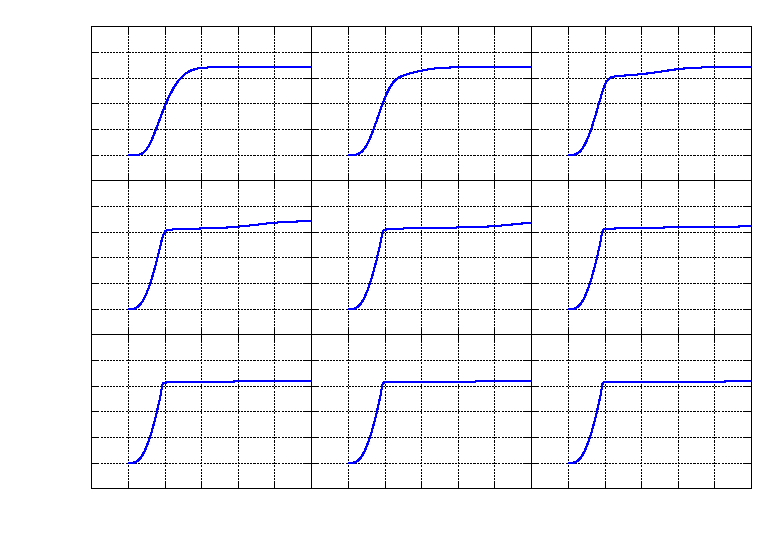
\includegraphics{mass_strong}}%
    \gplfronttext
  \end{picture}%
\endgroup

  \caption[Strong field results for the mass-aspect function $M(t,r)$.]{Strong field results for the mass-aspect function $M(t,r)$. The parameters of the run are $\eta=0.6$, $r_{0}=0$, $\delta=1$, $r_{\max}=64$, $w=0.15$, and $N_{r}=640$.}
  \label{fig:mass_strong}
\end{figure}

\subsubsection{Critical phenomena}

\begin{figure}[H]
  \centering
  % GNUPLOT: LaTeX picture with Postscript
\begingroup
  \makeatletter
  \providecommand\color[2][]{%
    \GenericError{(gnuplot) \space\space\space\@spaces}{%
      Package color not loaded in conjunction with
      terminal option `colourtext'%
    }{See the gnuplot documentation for explanation.%
    }{Either use 'blacktext' in gnuplot or load the package
      color.sty in LaTeX.}%
    \renewcommand\color[2][]{}%
  }%
  \providecommand\includegraphics[2][]{%
    \GenericError{(gnuplot) \space\space\space\@spaces}{%
      Package graphicx or graphics not loaded%
    }{See the gnuplot documentation for explanation.%
    }{The gnuplot epslatex terminal needs graphicx.sty or graphics.sty.}%
    \renewcommand\includegraphics[2][]{}%
  }%
  \providecommand\rotatebox[2]{#2}%
  \@ifundefined{ifGPcolor}{%
    \newif\ifGPcolor
    \GPcolorfalse
  }{}%
  \@ifundefined{ifGPblacktext}{%
    \newif\ifGPblacktext
    \GPblacktexttrue
  }{}%
  % define a \g@addto@macro without @ in the name:
  \let\gplgaddtomacro\g@addto@macro
  % define empty templates for all commands taking text:
  \gdef\gplbacktext{}%
  \gdef\gplfronttext{}%
  \makeatother
  \ifGPblacktext
    % no textcolor at all
    \def\colorrgb#1{}%
    \def\colorgray#1{}%
  \else
    % gray or color?
    \ifGPcolor
      \def\colorrgb#1{\color[rgb]{#1}}%
      \def\colorgray#1{\color[gray]{#1}}%
      \expandafter\def\csname LTw\endcsname{\color{white}}%
      \expandafter\def\csname LTb\endcsname{\color{black}}%
      \expandafter\def\csname LTa\endcsname{\color{black}}%
      \expandafter\def\csname LT0\endcsname{\color[rgb]{1,0,0}}%
      \expandafter\def\csname LT1\endcsname{\color[rgb]{0,1,0}}%
      \expandafter\def\csname LT2\endcsname{\color[rgb]{0,0,1}}%
      \expandafter\def\csname LT3\endcsname{\color[rgb]{1,0,1}}%
      \expandafter\def\csname LT4\endcsname{\color[rgb]{0,1,1}}%
      \expandafter\def\csname LT5\endcsname{\color[rgb]{1,1,0}}%
      \expandafter\def\csname LT6\endcsname{\color[rgb]{0,0,0}}%
      \expandafter\def\csname LT7\endcsname{\color[rgb]{1,0.3,0}}%
      \expandafter\def\csname LT8\endcsname{\color[rgb]{0.5,0.5,0.5}}%
    \else
      % gray
      \def\colorrgb#1{\color{black}}%
      \def\colorgray#1{\color[gray]{#1}}%
      \expandafter\def\csname LTw\endcsname{\color{white}}%
      \expandafter\def\csname LTb\endcsname{\color{black}}%
      \expandafter\def\csname LTa\endcsname{\color{black}}%
      \expandafter\def\csname LT0\endcsname{\color{black}}%
      \expandafter\def\csname LT1\endcsname{\color{black}}%
      \expandafter\def\csname LT2\endcsname{\color{black}}%
      \expandafter\def\csname LT3\endcsname{\color{black}}%
      \expandafter\def\csname LT4\endcsname{\color{black}}%
      \expandafter\def\csname LT5\endcsname{\color{black}}%
      \expandafter\def\csname LT6\endcsname{\color{black}}%
      \expandafter\def\csname LT7\endcsname{\color{black}}%
      \expandafter\def\csname LT8\endcsname{\color{black}}%
    \fi
  \fi
    \setlength{\unitlength}{0.0500bp}%
    \ifx\gptboxheight\undefined%
      \newlength{\gptboxheight}%
      \newlength{\gptboxwidth}%
      \newsavebox{\gptboxtext}%
    \fi%
    \setlength{\fboxrule}{0.5pt}%
    \setlength{\fboxsep}{1pt}%
\begin{picture}(7200.00,5040.00)%
    \gplgaddtomacro\gplbacktext{%
      \csname LTb\endcsname%%
      \put(588,3212){\makebox(0,0)[r]{\strut{}0.0}}%
      \csname LTb\endcsname%%
      \put(588,3666){\makebox(0,0)[r]{\strut{}$0.2$}}%
      \csname LTb\endcsname%%
      \put(588,4119){\makebox(0,0)[r]{\strut{}$0.4$}}%
      \csname LTb\endcsname%%
      \put(588,4573){\makebox(0,0)[r]{\strut{}$0.6$}}%
      \csname LTb\endcsname%%
      \put(1147,2879){\makebox(0,0){\strut{}$0$}}%
      \csname LTb\endcsname%%
      \put(2000,2879){\makebox(0,0){\strut{}$1$}}%
      \csname LTb\endcsname%%
      \put(2854,2879){\makebox(0,0){\strut{}$2$}}%
      \csname LTb\endcsname%%
      \put(3708,2879){\makebox(0,0){\strut{}$3$}}%
      \csname LTb\endcsname%%
      \put(4561,2879){\makebox(0,0){\strut{}$4$}}%
      \csname LTb\endcsname%%
      \put(5415,2879){\makebox(0,0){\strut{}$5$}}%
      \csname LTb\endcsname%%
      \put(6268,2879){\makebox(0,0){\strut{}$6$}}%
    }%
    \gplgaddtomacro\gplfronttext{%
      \csname LTb\endcsname%%
      \put(82,3892){\rotatebox{-270}{\makebox(0,0){\strut{}$\alpha_{\rm central}$}}}%
      \put(3707,569){\makebox(0,0){\strut{}$t$}}%
      \csname LTb\endcsname%%
      \put(5708,4458){\makebox(0,0)[r]{\strut{}$\eta = 0.3360583310$}}%
      \csname LTb\endcsname%%
      \put(5708,4238){\makebox(0,0)[r]{\strut{}$\eta = 0.3360583311$}}%
    }%
    \gplgaddtomacro\gplbacktext{%
      \csname LTb\endcsname%%
      \put(3935,1126){\makebox(0,0)[r]{\strut{}0.0}}%
      \csname LTb\endcsname%%
      \put(3935,1713){\makebox(0,0)[r]{\strut{}$0.1$}}%
      \csname LTb\endcsname%%
      \put(3935,2301){\makebox(0,0)[r]{\strut{}$0.2$}}%
      \csname LTb\endcsname%%
      \put(4471,788){\makebox(0,0){\strut{}$4.3$}}%
      \csname LTb\endcsname%%
      \put(5078,788){\makebox(0,0){\strut{}$4.6$}}%
      \csname LTb\endcsname%%
      \put(5684,788){\makebox(0,0){\strut{}$4.9$}}%
      \csname LTb\endcsname%%
      \put(6291,788){\makebox(0,0){\strut{}$5.2$}}%
    }%
    \gplgaddtomacro\gplfronttext{%
    }%
    \gplgaddtomacro\gplbacktext{%
      \csname LTb\endcsname%%
      \put(588,1114){\makebox(0,0)[r]{\strut{}0.00}}%
      \csname LTb\endcsname%%
      \put(588,1643){\makebox(0,0)[r]{\strut{}$0.05$}}%
      \csname LTb\endcsname%%
      \put(588,2172){\makebox(0,0)[r]{\strut{}0.10}}%
      \csname LTb\endcsname%%
      \put(884,788){\makebox(0,0){\strut{}5.230}}%
      \csname LTb\endcsname%%
      \put(2034,788){\makebox(0,0){\strut{}$5.265$}}%
      \csname LTb\endcsname%%
      \put(3183,788){\makebox(0,0){\strut{}5.300}}%
    }%
    \gplgaddtomacro\gplfronttext{%
    }%
    \gplbacktext
    \put(0,0){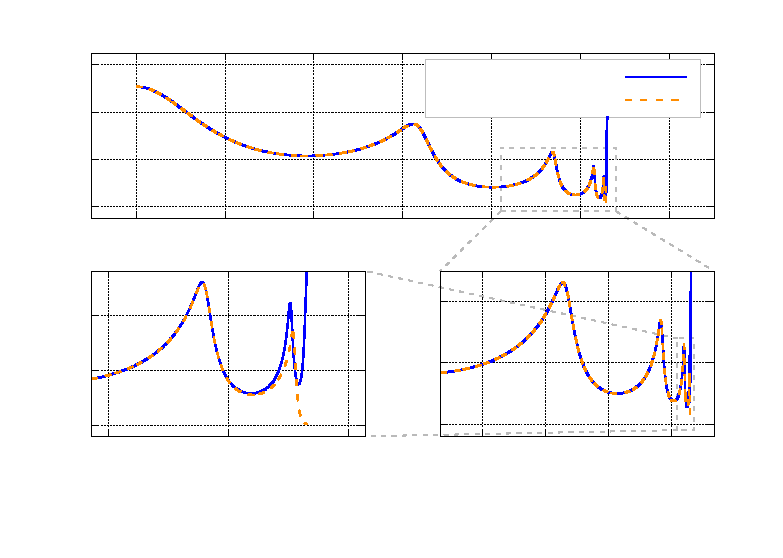
\includegraphics{resources/critical_lapse}}%
    \gplfronttext
  \end{picture}%
\endgroup

  \caption[$\alpha_{\rm central}$ results near criticality using a different grid setup.]{$\alpha_{\rm central}$ results near criticality using a different grid setup. The simulation parameters used were $N_{r}=320$, $w=0.08$, and $r_{\max}=16$. Note that we have fine-tuned the critical parameter to $\d\eta\sim10^{-13}$.}
  \label{fig:critical_alpha}
\end{figure}

The central energy density is then expected to have the behaviour

\eq{
\ln\lrpar{\rho^{\rm max}_{\rm central}} = C - 2\g\,z + A\sin\lrpar{\omega z + \varphi}\ ,\label{eq:fit_critical_exponent}
}

\n where $\g$ is the critical exponent, $\omega$ is the angular frequency of the oscillations, $\varphi$ the oscillation phase and $C$ and $A$ constants. The variable $z$ is defined as

\eq{
  z \equiv \ln\abs{\eta_{*}-\eta}\ ,
}

\n and $\eta<\eta_{*}$, since we are only evolving subcritical data. The angular frequency $\omega$ is related to the logarithmic period $\D$ via the relation

\eq{
  \omega = \frac{4\pi\g}{\D}\ ,\label{eq:universal_period_ito_omega}
}

\n and the oscillations are conjectured to have the universal oscillation period~\cite{PhysRevD.55.R440}

\eq{
  T = \frac{\D}{2\g} \approx 4.6\ .
}

To fit the numerical data with equation~\eqref{eq:fit_critical_exponent}, we fit the linear and oscillatory behaviours of $\ln\lrpar{\rho^{\rm max}_{\rm central}}$ separately. First, we drop the oscillatory term altogether and assume the original power law behaviour discovered by Choptuik

\eq{
  \rho^{\rm max}_{\rm central} \propto \abs{\eta_{*}-\eta}^{-2\g}\ ,
}

\n which results in the relation


\eq{
  \ln\lrpar{\rho^{\rm max}_{\rm central}} = C - 2\g\ln\abs{\eta_{*}-\eta}\ .\label{eq:fit_critical_exponent_linear}
}

\n We then use~\eqref{eq:fit_critical_exponent_linear} to obtain the parameters $\eta_{*}$, $\g$, and $C$ using {\tt SciPy}~\cite{2020SciPy-NMeth}. Having determined the linear behaviour of the function, we compute

\eq{
g(z) \equiv \ln\lrpar{\rho^{\rm max}_{\rm central}} - C + 2\g\ln(z)\ ,
}

\n using the known values of $\eta_{*}$, $\g$, and $C$ and the numerical data. We then expect that that the data points $g(z)$ can be well approximated by the oscillatory function in equation~\eqref{eq:fit_critical_exponent}. To determine the remaining fit parameters, we first perfom an estimate of $T_{\rm data}$, the period of oscillation of the energy density data. This was done by plotting $g(z)$ and visually estimating the value of $T_{\rm data}$. This analysis allowed us to estimate $T_{\rm data}\approx4.6$, in agreement with~\cite{PhysRevD.55.R440}. The value of $\omega$ was then computed from the period, allowing us to impose reliable bounds to the possible values of the angular frequency. Figure~\ref{fig:critical_exponent_oscillation} shows how we determined $T_{\rm data}$ and that the oscillatory function in equation~\eqref{eq:fit_critical_exponent} is adequate to approximate $g(z)$.

\begin{figure}[H]
  \centering
  % GNUPLOT: LaTeX picture with Postscript
\begingroup
  \makeatletter
  \providecommand\color[2][]{%
    \GenericError{(gnuplot) \space\space\space\@spaces}{%
      Package color not loaded in conjunction with
      terminal option `colourtext'%
    }{See the gnuplot documentation for explanation.%
    }{Either use 'blacktext' in gnuplot or load the package
      color.sty in LaTeX.}%
    \renewcommand\color[2][]{}%
  }%
  \providecommand\includegraphics[2][]{%
    \GenericError{(gnuplot) \space\space\space\@spaces}{%
      Package graphicx or graphics not loaded%
    }{See the gnuplot documentation for explanation.%
    }{The gnuplot epslatex terminal needs graphicx.sty or graphics.sty.}%
    \renewcommand\includegraphics[2][]{}%
  }%
  \providecommand\rotatebox[2]{#2}%
  \@ifundefined{ifGPcolor}{%
    \newif\ifGPcolor
    \GPcolorfalse
  }{}%
  \@ifundefined{ifGPblacktext}{%
    \newif\ifGPblacktext
    \GPblacktexttrue
  }{}%
  % define a \g@addto@macro without @ in the name:
  \let\gplgaddtomacro\g@addto@macro
  % define empty templates for all commands taking text:
  \gdef\gplbacktext{}%
  \gdef\gplfronttext{}%
  \makeatother
  \ifGPblacktext
    % no textcolor at all
    \def\colorrgb#1{}%
    \def\colorgray#1{}%
  \else
    % gray or color?
    \ifGPcolor
      \def\colorrgb#1{\color[rgb]{#1}}%
      \def\colorgray#1{\color[gray]{#1}}%
      \expandafter\def\csname LTw\endcsname{\color{white}}%
      \expandafter\def\csname LTb\endcsname{\color{black}}%
      \expandafter\def\csname LTa\endcsname{\color{black}}%
      \expandafter\def\csname LT0\endcsname{\color[rgb]{1,0,0}}%
      \expandafter\def\csname LT1\endcsname{\color[rgb]{0,1,0}}%
      \expandafter\def\csname LT2\endcsname{\color[rgb]{0,0,1}}%
      \expandafter\def\csname LT3\endcsname{\color[rgb]{1,0,1}}%
      \expandafter\def\csname LT4\endcsname{\color[rgb]{0,1,1}}%
      \expandafter\def\csname LT5\endcsname{\color[rgb]{1,1,0}}%
      \expandafter\def\csname LT6\endcsname{\color[rgb]{0,0,0}}%
      \expandafter\def\csname LT7\endcsname{\color[rgb]{1,0.3,0}}%
      \expandafter\def\csname LT8\endcsname{\color[rgb]{0.5,0.5,0.5}}%
    \else
      % gray
      \def\colorrgb#1{\color{black}}%
      \def\colorgray#1{\color[gray]{#1}}%
      \expandafter\def\csname LTw\endcsname{\color{white}}%
      \expandafter\def\csname LTb\endcsname{\color{black}}%
      \expandafter\def\csname LTa\endcsname{\color{black}}%
      \expandafter\def\csname LT0\endcsname{\color{black}}%
      \expandafter\def\csname LT1\endcsname{\color{black}}%
      \expandafter\def\csname LT2\endcsname{\color{black}}%
      \expandafter\def\csname LT3\endcsname{\color{black}}%
      \expandafter\def\csname LT4\endcsname{\color{black}}%
      \expandafter\def\csname LT5\endcsname{\color{black}}%
      \expandafter\def\csname LT6\endcsname{\color{black}}%
      \expandafter\def\csname LT7\endcsname{\color{black}}%
      \expandafter\def\csname LT8\endcsname{\color{black}}%
    \fi
  \fi
    \setlength{\unitlength}{0.0500bp}%
    \ifx\gptboxheight\undefined%
      \newlength{\gptboxheight}%
      \newlength{\gptboxwidth}%
      \newsavebox{\gptboxtext}%
    \fi%
    \setlength{\fboxrule}{0.5pt}%
    \setlength{\fboxsep}{1pt}%
\begin{picture}(7200.00,4320.00)%
    \gplgaddtomacro\gplbacktext{%
      \csname LTb\endcsname%%
      \put(588,907){\makebox(0,0)[r]{\strut{}$-0.75$}}%
      \csname LTb\endcsname%%
      \put(588,1382){\makebox(0,0)[r]{\strut{}$-0.50$}}%
      \csname LTb\endcsname%%
      \put(588,1857){\makebox(0,0)[r]{\strut{}$-0.25$}}%
      \csname LTb\endcsname%%
      \put(588,2332){\makebox(0,0)[r]{\strut{}$0.00$}}%
      \csname LTb\endcsname%%
      \put(588,2807){\makebox(0,0)[r]{\strut{}$0.25$}}%
      \csname LTb\endcsname%%
      \put(588,3282){\makebox(0,0)[r]{\strut{}$0.50$}}%
      \csname LTb\endcsname%%
      \put(588,3757){\makebox(0,0)[r]{\strut{}$0.75$}}%
      \csname LTb\endcsname%%
      \put(1172,212){\makebox(0,0){\strut{}$-30$}}%
      \csname LTb\endcsname%%
      \put(1738,212){\makebox(0,0){\strut{}$-25$}}%
      \csname LTb\endcsname%%
      \put(2304,212){\makebox(0,0){\strut{}$-20$}}%
      \csname LTb\endcsname%%
      \put(2869,212){\makebox(0,0){\strut{}$-15$}}%
      \csname LTb\endcsname%%
      \put(3435,212){\makebox(0,0){\strut{}$-10$}}%
    }%
    \gplgaddtomacro\gplfronttext{%
      \csname LTb\endcsname%%
      \put(-182,2332){\rotatebox{-270}{\makebox(0,0){\strut{}$\ln\left(\rho^{\max}_{\rm central}\right) - C + 2\gamma\ln\left|\eta_{*}-\eta\right|$}}}%
      \put(3887,-118){\makebox(0,0){\strut{}$\ln\left(\eta_{*}-\eta\right)$}}%
    }%
    \gplgaddtomacro\gplbacktext{%
      \csname LTb\endcsname%%
      \put(3756,907){\makebox(0,0)[r]{\strut{}}}%
      \csname LTb\endcsname%%
      \put(3756,1382){\makebox(0,0)[r]{\strut{}}}%
      \csname LTb\endcsname%%
      \put(3756,1857){\makebox(0,0)[r]{\strut{}}}%
      \csname LTb\endcsname%%
      \put(3756,2332){\makebox(0,0)[r]{\strut{}}}%
      \csname LTb\endcsname%%
      \put(3756,2807){\makebox(0,0)[r]{\strut{}}}%
      \csname LTb\endcsname%%
      \put(3756,3282){\makebox(0,0)[r]{\strut{}}}%
      \csname LTb\endcsname%%
      \put(3756,3757){\makebox(0,0)[r]{\strut{}}}%
      \csname LTb\endcsname%%
      \put(4340,212){\makebox(0,0){\strut{}$-30$}}%
      \csname LTb\endcsname%%
      \put(4906,212){\makebox(0,0){\strut{}$-25$}}%
      \csname LTb\endcsname%%
      \put(5472,212){\makebox(0,0){\strut{}$-20$}}%
      \csname LTb\endcsname%%
      \put(6037,212){\makebox(0,0){\strut{}$-15$}}%
      \csname LTb\endcsname%%
      \put(6603,212){\makebox(0,0){\strut{}$-10$}}%
    }%
    \gplgaddtomacro\gplfronttext{%
      \csname LTb\endcsname%%
      \put(6068,4059){\makebox(0,0)[r]{\strut{}Data points}}%
      \csname LTb\endcsname%%
      \put(6068,3839){\makebox(0,0)[r]{\strut{}Fitting curve}}%
    }%
    \gplbacktext
    \put(0,0){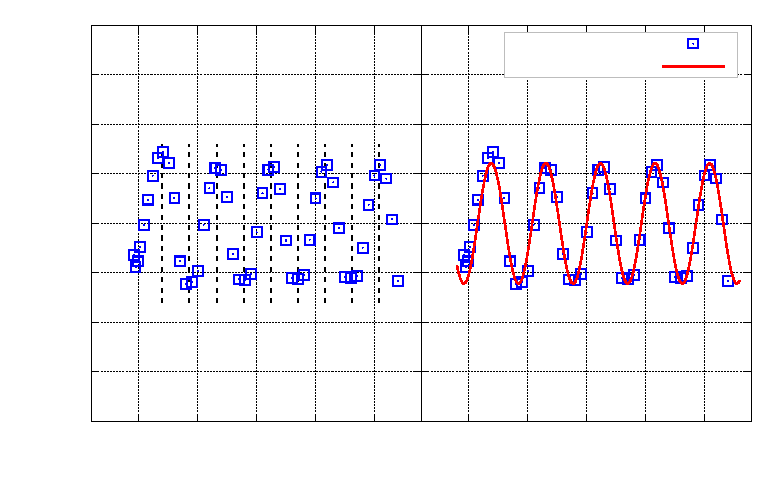
\includegraphics{resources/critical_exponent_oscillation}}%
    \gplfronttext
  \end{picture}%
\endgroup

  \caption[Visual estimation of the oscillation period and fit.]{Visual estimation of the oscillation period (left) and fitting result (right). On the left panel, the vertical dashed lines are equally spaced with $\D z = 2.3$ and starting at $z=-28$. This allows us to visually estimate the period of oscillation to be $T_{\rm data}\approx4.6$, as expected. With this estimate of $T_{\rm data}$, we compute $\omega = \frac{2\pi}{T_{\rm data}}$ and use the value obtained to restringe our search for the fitting value of $\omega$. The function $A\sin\lrpar{\omega z+\varphi}$ is then used to fit the data points, and the result is displayed on the right panel. The values of $A$, $\omega$, and $\varphi$ are presented in table~\ref{tab:fit_critical_exponent}.}
  \label{fig:critical_exponent_oscillation}
\end{figure}

Having found all the fitting parameters, whose values are shown in table~\ref{tab:fit_critical_exponent}, we use equation~\eqref{eq:fit_critical_exponent} to fit the numerical data. The result of this fit is presented in figure~\ref{fig:critical_exponent}. We emphasize that the parameter values obtained are in excellent agreement with the literature~\cite{PhysRevLett.70.9,Baumgarte_2018,PhysRevD.55.R440,PhysRevD.92.084037}.

\begin{table}[ht]
  \centering
  \begin{tabular}{cccccc}
    \hline
    \hline
    $\g$ & $\omega$ & $\D$~\eqref{eq:universal_period_ito_omega} & $C$ & $A$ & $\varphi$\\
    \hline
    0.374 & 1.36 & 3.47 & -2.54 & 0.304 & 1.96\\
    \hline
    \hline
  \end{tabular}
  \caption[Fit parameters for the behaviour of the central energy density in a series of subcritical runs.]{Fit parameters obtained for equation~\eqref{eq:fit_critical_exponent} in a series of subcritical runs. The value of $\D$ has been computed using~\eqref{eq:universal_period_ito_omega}.}
  \label{tab:fit_critical_exponent}
\end{table}

\begin{figure}[H]
  \centering
  % GNUPLOT: LaTeX picture with Postscript
\begingroup
  \makeatletter
  \providecommand\color[2][]{%
    \GenericError{(gnuplot) \space\space\space\@spaces}{%
      Package color not loaded in conjunction with
      terminal option `colourtext'%
    }{See the gnuplot documentation for explanation.%
    }{Either use 'blacktext' in gnuplot or load the package
      color.sty in LaTeX.}%
    \renewcommand\color[2][]{}%
  }%
  \providecommand\includegraphics[2][]{%
    \GenericError{(gnuplot) \space\space\space\@spaces}{%
      Package graphicx or graphics not loaded%
    }{See the gnuplot documentation for explanation.%
    }{The gnuplot epslatex terminal needs graphicx.sty or graphics.sty.}%
    \renewcommand\includegraphics[2][]{}%
  }%
  \providecommand\rotatebox[2]{#2}%
  \@ifundefined{ifGPcolor}{%
    \newif\ifGPcolor
    \GPcolorfalse
  }{}%
  \@ifundefined{ifGPblacktext}{%
    \newif\ifGPblacktext
    \GPblacktexttrue
  }{}%
  % define a \g@addto@macro without @ in the name:
  \let\gplgaddtomacro\g@addto@macro
  % define empty templates for all commands taking text:
  \gdef\gplbacktext{}%
  \gdef\gplfronttext{}%
  \makeatother
  \ifGPblacktext
    % no textcolor at all
    \def\colorrgb#1{}%
    \def\colorgray#1{}%
  \else
    % gray or color?
    \ifGPcolor
      \def\colorrgb#1{\color[rgb]{#1}}%
      \def\colorgray#1{\color[gray]{#1}}%
      \expandafter\def\csname LTw\endcsname{\color{white}}%
      \expandafter\def\csname LTb\endcsname{\color{black}}%
      \expandafter\def\csname LTa\endcsname{\color{black}}%
      \expandafter\def\csname LT0\endcsname{\color[rgb]{1,0,0}}%
      \expandafter\def\csname LT1\endcsname{\color[rgb]{0,1,0}}%
      \expandafter\def\csname LT2\endcsname{\color[rgb]{0,0,1}}%
      \expandafter\def\csname LT3\endcsname{\color[rgb]{1,0,1}}%
      \expandafter\def\csname LT4\endcsname{\color[rgb]{0,1,1}}%
      \expandafter\def\csname LT5\endcsname{\color[rgb]{1,1,0}}%
      \expandafter\def\csname LT6\endcsname{\color[rgb]{0,0,0}}%
      \expandafter\def\csname LT7\endcsname{\color[rgb]{1,0.3,0}}%
      \expandafter\def\csname LT8\endcsname{\color[rgb]{0.5,0.5,0.5}}%
    \else
      % gray
      \def\colorrgb#1{\color{black}}%
      \def\colorgray#1{\color[gray]{#1}}%
      \expandafter\def\csname LTw\endcsname{\color{white}}%
      \expandafter\def\csname LTb\endcsname{\color{black}}%
      \expandafter\def\csname LTa\endcsname{\color{black}}%
      \expandafter\def\csname LT0\endcsname{\color{black}}%
      \expandafter\def\csname LT1\endcsname{\color{black}}%
      \expandafter\def\csname LT2\endcsname{\color{black}}%
      \expandafter\def\csname LT3\endcsname{\color{black}}%
      \expandafter\def\csname LT4\endcsname{\color{black}}%
      \expandafter\def\csname LT5\endcsname{\color{black}}%
      \expandafter\def\csname LT6\endcsname{\color{black}}%
      \expandafter\def\csname LT7\endcsname{\color{black}}%
      \expandafter\def\csname LT8\endcsname{\color{black}}%
    \fi
  \fi
    \setlength{\unitlength}{0.0500bp}%
    \ifx\gptboxheight\undefined%
      \newlength{\gptboxheight}%
      \newlength{\gptboxwidth}%
      \newsavebox{\gptboxtext}%
    \fi%
    \setlength{\fboxrule}{0.5pt}%
    \setlength{\fboxsep}{1pt}%
\begin{picture}(7200.00,5040.00)%
    \gplgaddtomacro\gplbacktext{%
      \csname LTb\endcsname%%
      \put(682,1218){\makebox(0,0)[r]{\strut{}$5$}}%
      \csname LTb\endcsname%%
      \put(682,2247){\makebox(0,0)[r]{\strut{}$10$}}%
      \csname LTb\endcsname%%
      \put(682,3276){\makebox(0,0)[r]{\strut{}$15$}}%
      \csname LTb\endcsname%%
      \put(682,4305){\makebox(0,0)[r]{\strut{}$20$}}%
      \csname LTb\endcsname%%
      \put(1505,484){\makebox(0,0){\strut{}$-30$}}%
      \csname LTb\endcsname%%
      \put(2657,484){\makebox(0,0){\strut{}$-25$}}%
      \csname LTb\endcsname%%
      \put(3809,484){\makebox(0,0){\strut{}$-20$}}%
      \csname LTb\endcsname%%
      \put(4960,484){\makebox(0,0){\strut{}$-15$}}%
      \csname LTb\endcsname%%
      \put(6112,484){\makebox(0,0){\strut{}$-10$}}%
    }%
    \gplgaddtomacro\gplfronttext{%
      \csname LTb\endcsname%%
      \put(308,2761){\rotatebox{-270}{\makebox(0,0){\strut{}$\ln\left(\rho^{\max}_{\rm central}\right)$}}}%
      \put(3808,154){\makebox(0,0){\strut{}$\ln\left(\eta_{*}-\eta\right)$}}%
      \csname LTb\endcsname%%
      \put(5816,4646){\makebox(0,0)[r]{\strut{}Data points}}%
      \csname LTb\endcsname%%
      \put(5816,4426){\makebox(0,0)[r]{\strut{}Fitting curve}}%
    }%
    \gplbacktext
    \put(0,0){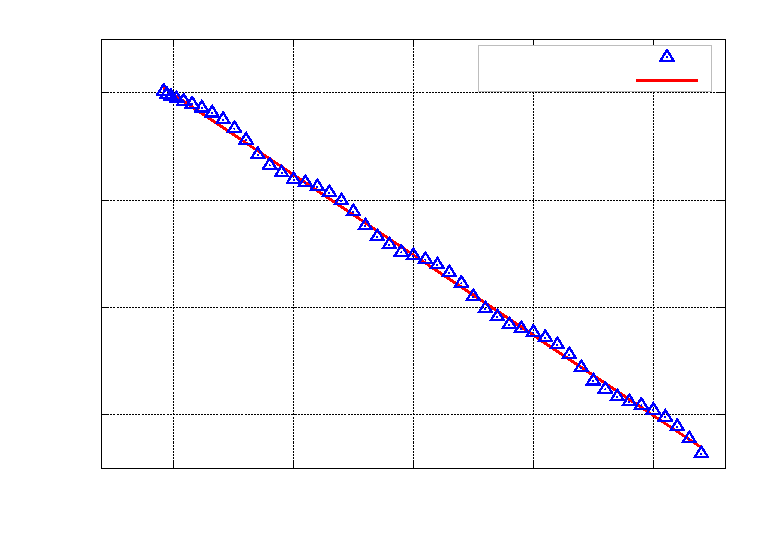
\includegraphics{resources/critical_exponent}}%
    \gplfronttext
  \end{picture}%
\endgroup

  \caption[Central energy density near criticality.]{The plot shows the maximum central density for several subcritical runs. The critical exponent $\gamma\approx0.374$, oscillation period $T_{\rm data}\approx4.6$, and logarithmic oscillation period $\D\approx3.47$, obtained using the fitting function~\eqref{eq:fit_critical_exponent}, are all in excellent agreement with the literature.}
  \label{fig:critical_exponent}
\end{figure}

We now show how the scalar field behaves near criticality. We start by computing the proper time, $\tau$, which in terms of the coordinate time, $t$, is given by

\eq{
  \tau(t) = \int_{0}^{t}\a\lrpar{t^{\prime}}dt^{\prime}\ .
}

\n Since we are interested in central values, we only need to evaluate the proper time at the origin. In practice, we evaluated it using

\eq{
  \tau_{n} = \left\{
  \begin{matrix}
    0 & \text{, if } n=0\\
    \tau_{n-1} + \left(t_{n}-t_{n-1}\right)\lrpar{\frac{\alpha^{n}_{0}+\alpha^{n-1}_{0}}{2}} & \text{, if } n\neq0
  \end{matrix}
  \right.\ ,
}

\n where $\tau_{n}\equiv\tau(t_{n})$ and $t_{n}\equiv n\cdot\dt$. The behaviour of the scalar field as a function of proper time is displayed in figure~\ref{fig:accumulation_tau}.

We now define the logarithmic time variable

\eq{
  \Lambda \equiv -\ln\lrpar{\tau_{*}-\tau}\ ,\label{eq:log_proper_time}
}

\n where $\tau_{*}$ is referred to as the \emph{accumulation time}. Now let $\tau_{n}$ represent the number of times $\phi_{\rm central}$ crosses zero throughout the simulation. Consider still two pairs of crossings $\lrpar{\tau_{n},\tau_{n+1}}$ and $\lrpar{\tau_{m},\tau_{m+1}}$ and assume that \emph{in the logarithmic time} $\Lambda$ these two pair of points correspond to the same half-period of oscillation $\frac{\D}{2}$, i.e.

\eq{
  \Lambda_{n+1}-\Lambda_{n} = \frac{\D}{2} = \Lambda_{m+1}-\Lambda_{m}\ ,\label{eq:lambda_diff}
}

\n where $\Lambda_{n} \equiv \Lambda\lrpar{\tau_{n}}$. From equations~\eqref{eq:log_proper_time} and~\eqref{eq:lambda_diff} we can estimate the accumulation time $\tau_{*}$ using

\eq{
  \ln\lrpar{\frac{\tau_{*}-\tau_{n}}{\tau_{*}-\tau_{n+1}}} = \ln\lrpar{\frac{\tau_{*}-\tau_{m}}{\tau_{*}-\tau_{m+1}}} \implies \tau_{*} = \frac{\tau_{n}\tau_{m+1}-\tau_{m}\tau_{n+1}}{\tau_{n}-\tau_{n+1}-\tau_{m}+\tau_{m+1}}\ . \label{eq:tau_star}
}

Using the same train of thought, we can use a single pair $\lrpar{\tau_{n},\tau_{n+1}}$ to estimate the period $\D$ using

\eq{
  \frac{\D}{2} = -\lrsquare{\ln\lrpar{\tau_{*}-\tau_{n+1}} - \ln\lrpar{\tau_{*}-\tau_{n}}} \implies \D = 2\ln\lrpar{ \frac{\tau_{*}-\tau_{n}}{\tau_{*}-\tau_{n+1}} }\ .\label{eq:Delta_method2}
}


%% tau = 0.625914 | diff = 0.483540 | Lambda = 0.504722  | Diff(0,1) = 0.483540 | Delta(0,1) = 3.23
%% tau = 1.109454 | diff = 0.098750 | Lambda = 2.119155  | Diff(1,2) = 0.098750 | Delta(1,2) = 3.45
%% tau = 1.208204 | diff = 0.017499 | Lambda = 3.845173  | Diff(2,3) = 0.017499 | Delta(2,3) = 3.41
%% tau = 1.225703 | diff = 0.003190 | Lambda = 5.550879  | Diff(3,4) = 0.003190 | Delta(3,4) = 3.44
%% tau = 1.228893 | diff = 0.000565 | Lambda = 7.273271  | Diff(4,5) = 0.000565 | Delta(4,5) = 3.37
%% tau = 1.229458 | diff = 0.000106 | Lambda = 8.958907  | Diff(5,6) = 0.000106 | Delta(5,6) = 3.46
%% tau = 1.229564 | diff = 0.000054 | Lambda = 10.689805 |                      | Delta(avg) = 3.43
\begin{table}[ht]
  \centering
  \begin{tabular}{c|ccccccc}
    \hline
    \hline
    $n$ & $0$ & $1$ & $2$ & $3$ & $4$ & $5$ & $6$\\
    \hline
    $\tau_{n}$ & 0.625914 & 1.109454 & 1.208204 & 1.225703 & 1.228893 & 1.229458 & 1.229564\\
    $\Lambda_{n}$ & 0.504722 & 2.119155 & 3.845173 & 5.550879 & 7.273271 & 8.958907 & 10.689805\\
    \hline
    \hline
    \multirow{2}{*}{Eq.~\eqref{eq:Delta_method2}} & $\D_{0,1}$ & $\D_{1,2}$ & $\D_{2,3}$ & $\D_{3,4}$ & $\D_{4,5}$ & $\D_{5,6}$ & $\D_{\rm avg}$\\
    \cline{2-8}
    & 3.23 & 3.45 & 3.41 & 3.44 & 3.37 & 3.46 & 3.43\\
    \hline
    \hline
  \end{tabular}
  \caption[Values of proper time and logarithmic proper time used to estimate the universal oscillation period $\D$.]{Values of proper time, $\tau$, and logarithmic proper time, $\Lambda$, for which the scalar field crosses zero. From these values we compute the period $\Delta$ using equation~\eqref{eq:Delta_method2}. The notation $\Delta_{n,n+1}$ indicates which pair $\lrpar{\tau_{n},\tau_{n+1}}$ was used to estimate $\Delta$. The average value $\D_{\rm avg}$ does not take into account $\D_{0,1}$ because we noticed that the scalar field was still transitioning to the critical regime.}
  \label{tab:accumulation_time}
\end{table}

\begin{figure}[ht]
  \centering
  % GNUPLOT: LaTeX picture with Postscript
\begingroup
  \makeatletter
  \providecommand\color[2][]{%
    \GenericError{(gnuplot) \space\space\space\@spaces}{%
      Package color not loaded in conjunction with
      terminal option `colourtext'%
    }{See the gnuplot documentation for explanation.%
    }{Either use 'blacktext' in gnuplot or load the package
      color.sty in LaTeX.}%
    \renewcommand\color[2][]{}%
  }%
  \providecommand\includegraphics[2][]{%
    \GenericError{(gnuplot) \space\space\space\@spaces}{%
      Package graphicx or graphics not loaded%
    }{See the gnuplot documentation for explanation.%
    }{The gnuplot epslatex terminal needs graphicx.sty or graphics.sty.}%
    \renewcommand\includegraphics[2][]{}%
  }%
  \providecommand\rotatebox[2]{#2}%
  \@ifundefined{ifGPcolor}{%
    \newif\ifGPcolor
    \GPcolorfalse
  }{}%
  \@ifundefined{ifGPblacktext}{%
    \newif\ifGPblacktext
    \GPblacktexttrue
  }{}%
  % define a \g@addto@macro without @ in the name:
  \let\gplgaddtomacro\g@addto@macro
  % define empty templates for all commands taking text:
  \gdef\gplbacktext{}%
  \gdef\gplfronttext{}%
  \makeatother
  \ifGPblacktext
    % no textcolor at all
    \def\colorrgb#1{}%
    \def\colorgray#1{}%
  \else
    % gray or color?
    \ifGPcolor
      \def\colorrgb#1{\color[rgb]{#1}}%
      \def\colorgray#1{\color[gray]{#1}}%
      \expandafter\def\csname LTw\endcsname{\color{white}}%
      \expandafter\def\csname LTb\endcsname{\color{black}}%
      \expandafter\def\csname LTa\endcsname{\color{black}}%
      \expandafter\def\csname LT0\endcsname{\color[rgb]{1,0,0}}%
      \expandafter\def\csname LT1\endcsname{\color[rgb]{0,1,0}}%
      \expandafter\def\csname LT2\endcsname{\color[rgb]{0,0,1}}%
      \expandafter\def\csname LT3\endcsname{\color[rgb]{1,0,1}}%
      \expandafter\def\csname LT4\endcsname{\color[rgb]{0,1,1}}%
      \expandafter\def\csname LT5\endcsname{\color[rgb]{1,1,0}}%
      \expandafter\def\csname LT6\endcsname{\color[rgb]{0,0,0}}%
      \expandafter\def\csname LT7\endcsname{\color[rgb]{1,0.3,0}}%
      \expandafter\def\csname LT8\endcsname{\color[rgb]{0.5,0.5,0.5}}%
    \else
      % gray
      \def\colorrgb#1{\color{black}}%
      \def\colorgray#1{\color[gray]{#1}}%
      \expandafter\def\csname LTw\endcsname{\color{white}}%
      \expandafter\def\csname LTb\endcsname{\color{black}}%
      \expandafter\def\csname LTa\endcsname{\color{black}}%
      \expandafter\def\csname LT0\endcsname{\color{black}}%
      \expandafter\def\csname LT1\endcsname{\color{black}}%
      \expandafter\def\csname LT2\endcsname{\color{black}}%
      \expandafter\def\csname LT3\endcsname{\color{black}}%
      \expandafter\def\csname LT4\endcsname{\color{black}}%
      \expandafter\def\csname LT5\endcsname{\color{black}}%
      \expandafter\def\csname LT6\endcsname{\color{black}}%
      \expandafter\def\csname LT7\endcsname{\color{black}}%
      \expandafter\def\csname LT8\endcsname{\color{black}}%
    \fi
  \fi
    \setlength{\unitlength}{0.0500bp}%
    \ifx\gptboxheight\undefined%
      \newlength{\gptboxheight}%
      \newlength{\gptboxwidth}%
      \newsavebox{\gptboxtext}%
    \fi%
    \setlength{\fboxrule}{0.5pt}%
    \setlength{\fboxsep}{1pt}%
\begin{picture}(7200.00,5040.00)%
    \gplgaddtomacro\gplbacktext{%
      \csname LTb\endcsname%%
      \put(946,998){\makebox(0,0)[r]{\strut{}$-0.6$}}%
      \csname LTb\endcsname%%
      \put(946,1586){\makebox(0,0)[r]{\strut{}$-0.4$}}%
      \csname LTb\endcsname%%
      \put(946,2174){\makebox(0,0)[r]{\strut{}$-0.2$}}%
      \csname LTb\endcsname%%
      \put(946,2762){\makebox(0,0)[r]{\strut{}$0.0$}}%
      \csname LTb\endcsname%%
      \put(946,3349){\makebox(0,0)[r]{\strut{}$0.2$}}%
      \csname LTb\endcsname%%
      \put(946,3937){\makebox(0,0)[r]{\strut{}$0.4$}}%
      \csname LTb\endcsname%%
      \put(946,4525){\makebox(0,0)[r]{\strut{}$0.6$}}%
      \csname LTb\endcsname%%
      \put(1487,484){\makebox(0,0){\strut{}$0.0$}}%
      \csname LTb\endcsname%%
      \put(2714,484){\makebox(0,0){\strut{}$0.3$}}%
      \csname LTb\endcsname%%
      \put(3940,484){\makebox(0,0){\strut{}$0.6$}}%
      \csname LTb\endcsname%%
      \put(5167,484){\makebox(0,0){\strut{}$0.9$}}%
      \csname LTb\endcsname%%
      \put(6394,484){\makebox(0,0){\strut{}$1.2$}}%
    }%
    \gplgaddtomacro\gplfronttext{%
      \csname LTb\endcsname%%
      \put(308,2761){\rotatebox{-270}{\makebox(0,0){\strut{}$\phi_{\rm central}$}}}%
      \put(3940,154){\makebox(0,0){\strut{}$\tau$}}%
    }%
    \gplbacktext
    \put(0,0){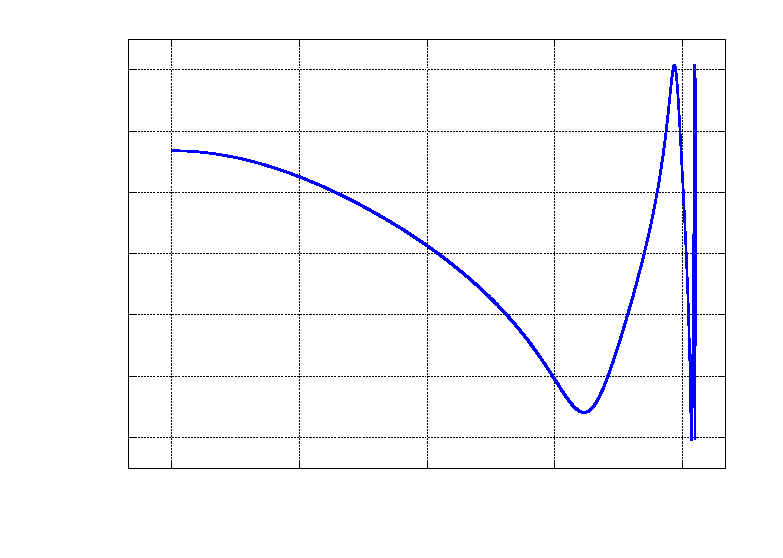
\includegraphics{resources/accumulation_tau}}%
    \gplfronttext
  \end{picture}%
\endgroup

  \caption[Central value of the scalar field, $\phi_{\rm central}$, near criticality as a function of proper time, $\tau$.]{Central value of the scalar field, $\phi_{\rm central}$, near criticality as a function of proper time, $\tau$.}
  \label{fig:accumulation_tau}
\end{figure}

\begin{figure}[htt]
  \centering
  % GNUPLOT: LaTeX picture with Postscript
\begingroup
  \makeatletter
  \providecommand\color[2][]{%
    \GenericError{(gnuplot) \space\space\space\@spaces}{%
      Package color not loaded in conjunction with
      terminal option `colourtext'%
    }{See the gnuplot documentation for explanation.%
    }{Either use 'blacktext' in gnuplot or load the package
      color.sty in LaTeX.}%
    \renewcommand\color[2][]{}%
  }%
  \providecommand\includegraphics[2][]{%
    \GenericError{(gnuplot) \space\space\space\@spaces}{%
      Package graphicx or graphics not loaded%
    }{See the gnuplot documentation for explanation.%
    }{The gnuplot epslatex terminal needs graphicx.sty or graphics.sty.}%
    \renewcommand\includegraphics[2][]{}%
  }%
  \providecommand\rotatebox[2]{#2}%
  \@ifundefined{ifGPcolor}{%
    \newif\ifGPcolor
    \GPcolorfalse
  }{}%
  \@ifundefined{ifGPblacktext}{%
    \newif\ifGPblacktext
    \GPblacktexttrue
  }{}%
  % define a \g@addto@macro without @ in the name:
  \let\gplgaddtomacro\g@addto@macro
  % define empty templates for all commands taking text:
  \gdef\gplbacktext{}%
  \gdef\gplfronttext{}%
  \makeatother
  \ifGPblacktext
    % no textcolor at all
    \def\colorrgb#1{}%
    \def\colorgray#1{}%
  \else
    % gray or color?
    \ifGPcolor
      \def\colorrgb#1{\color[rgb]{#1}}%
      \def\colorgray#1{\color[gray]{#1}}%
      \expandafter\def\csname LTw\endcsname{\color{white}}%
      \expandafter\def\csname LTb\endcsname{\color{black}}%
      \expandafter\def\csname LTa\endcsname{\color{black}}%
      \expandafter\def\csname LT0\endcsname{\color[rgb]{1,0,0}}%
      \expandafter\def\csname LT1\endcsname{\color[rgb]{0,1,0}}%
      \expandafter\def\csname LT2\endcsname{\color[rgb]{0,0,1}}%
      \expandafter\def\csname LT3\endcsname{\color[rgb]{1,0,1}}%
      \expandafter\def\csname LT4\endcsname{\color[rgb]{0,1,1}}%
      \expandafter\def\csname LT5\endcsname{\color[rgb]{1,1,0}}%
      \expandafter\def\csname LT6\endcsname{\color[rgb]{0,0,0}}%
      \expandafter\def\csname LT7\endcsname{\color[rgb]{1,0.3,0}}%
      \expandafter\def\csname LT8\endcsname{\color[rgb]{0.5,0.5,0.5}}%
    \else
      % gray
      \def\colorrgb#1{\color{black}}%
      \def\colorgray#1{\color[gray]{#1}}%
      \expandafter\def\csname LTw\endcsname{\color{white}}%
      \expandafter\def\csname LTb\endcsname{\color{black}}%
      \expandafter\def\csname LTa\endcsname{\color{black}}%
      \expandafter\def\csname LT0\endcsname{\color{black}}%
      \expandafter\def\csname LT1\endcsname{\color{black}}%
      \expandafter\def\csname LT2\endcsname{\color{black}}%
      \expandafter\def\csname LT3\endcsname{\color{black}}%
      \expandafter\def\csname LT4\endcsname{\color{black}}%
      \expandafter\def\csname LT5\endcsname{\color{black}}%
      \expandafter\def\csname LT6\endcsname{\color{black}}%
      \expandafter\def\csname LT7\endcsname{\color{black}}%
      \expandafter\def\csname LT8\endcsname{\color{black}}%
    \fi
  \fi
    \setlength{\unitlength}{0.0500bp}%
    \ifx\gptboxheight\undefined%
      \newlength{\gptboxheight}%
      \newlength{\gptboxwidth}%
      \newsavebox{\gptboxtext}%
    \fi%
    \setlength{\fboxrule}{0.5pt}%
    \setlength{\fboxsep}{1pt}%
\begin{picture}(7200.00,5040.00)%
    \gplgaddtomacro\gplbacktext{%
      \csname LTb\endcsname%%
      \put(946,998){\makebox(0,0)[r]{\strut{}$-0.6$}}%
      \csname LTb\endcsname%%
      \put(946,1586){\makebox(0,0)[r]{\strut{}$-0.4$}}%
      \csname LTb\endcsname%%
      \put(946,2174){\makebox(0,0)[r]{\strut{}$-0.2$}}%
      \csname LTb\endcsname%%
      \put(946,2762){\makebox(0,0)[r]{\strut{}$0.0$}}%
      \csname LTb\endcsname%%
      \put(946,3349){\makebox(0,0)[r]{\strut{}$0.2$}}%
      \csname LTb\endcsname%%
      \put(946,3937){\makebox(0,0)[r]{\strut{}$0.4$}}%
      \csname LTb\endcsname%%
      \put(946,4525){\makebox(0,0)[r]{\strut{}$0.6$}}%
      \csname LTb\endcsname%%
      \put(1896,484){\makebox(0,0){\strut{}$0.0$}}%
      \csname LTb\endcsname%%
      \put(2918,484){\makebox(0,0){\strut{}$2.5$}}%
      \csname LTb\endcsname%%
      \put(3941,484){\makebox(0,0){\strut{}$5.0$}}%
      \csname LTb\endcsname%%
      \put(4963,484){\makebox(0,0){\strut{}$7.5$}}%
      \csname LTb\endcsname%%
      \put(5985,484){\makebox(0,0){\strut{}$10.0$}}%
      \put(1857,2027){\makebox(0,0){\strut{}$n=0$}}%
      \put(2517,3496){\makebox(0,0){\strut{}$n=1$}}%
      \put(3223,2027){\makebox(0,0){\strut{}$n=2$}}%
      \put(3920,3496){\makebox(0,0){\strut{}$n=3$}}%
      \put(4625,2027){\makebox(0,0){\strut{}$n=4$}}%
      \put(5314,3496){\makebox(0,0){\strut{}$n=5$}}%
      \put(6022,2027){\makebox(0,0){\strut{}$n=6$}}%
    }%
    \gplgaddtomacro\gplfronttext{%
      \csname LTb\endcsname%%
      \put(308,2761){\rotatebox{-270}{\makebox(0,0){\strut{}$\phi_{\rm central}$}}}%
      \put(3940,154){\makebox(0,0){\strut{}$\Lambda$}}%
    }%
    \gplbacktext
    \put(0,0){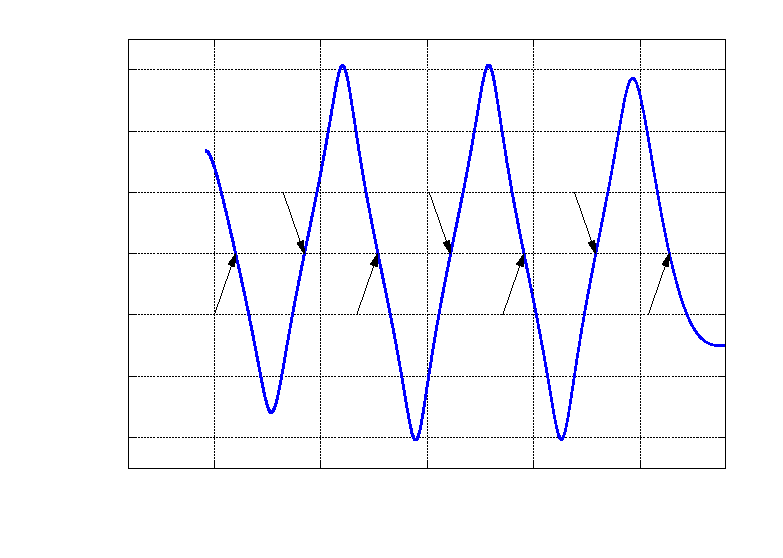
\includegraphics{resources/accumulation_Lambda}}%
    \gplfronttext
  \end{picture}%
\endgroup

  \caption[Central value of the scalar field, $\phi_{\rm central}$, near criticality as a function of logarithmic proper time, $\Lambda$.]{Same as figure~\ref{fig:accumulation_tau}, but the $x$-axis is now the logarithmic proper time\linebreak $\Lambda\equiv-\ln\lrpar{\tau_{*}-\tau}$. The accumulation time, $\tau_{*}$, was determined as the average value obtained from equation~\eqref{eq:tau_star} after using all possible pairs $\lrpar{\tau_{n},\tau_{n+1}}$ for which the scalar field was already in the critical regime. The figure also displays the number of times the central value of the scalar field changes sign over the evolution. The average oscillation period was estimated to be $\D \approx 3.43$, in agreement with the literature. We also observe that the central value of the scalar field oscillates in the interval $\lrpar{-0.61,0.61}$, consistent with what was found in~\cite{PhysRevLett.70.9,PhysRevD.92.084037,Baumgarte_2018}.}
  \label{fig:accumulation_Lambda}
\end{figure}

\subsubsection{Universality}

\begin{figure}[H]
  \centering
  % GNUPLOT: LaTeX picture with Postscript
\begingroup
  \makeatletter
  \providecommand\color[2][]{%
    \GenericError{(gnuplot) \space\space\space\@spaces}{%
      Package color not loaded in conjunction with
      terminal option `colourtext'%
    }{See the gnuplot documentation for explanation.%
    }{Either use 'blacktext' in gnuplot or load the package
      color.sty in LaTeX.}%
    \renewcommand\color[2][]{}%
  }%
  \providecommand\includegraphics[2][]{%
    \GenericError{(gnuplot) \space\space\space\@spaces}{%
      Package graphicx or graphics not loaded%
    }{See the gnuplot documentation for explanation.%
    }{The gnuplot epslatex terminal needs graphicx.sty or graphics.sty.}%
    \renewcommand\includegraphics[2][]{}%
  }%
  \providecommand\rotatebox[2]{#2}%
  \@ifundefined{ifGPcolor}{%
    \newif\ifGPcolor
    \GPcolorfalse
  }{}%
  \@ifundefined{ifGPblacktext}{%
    \newif\ifGPblacktext
    \GPblacktexttrue
  }{}%
  % define a \g@addto@macro without @ in the name:
  \let\gplgaddtomacro\g@addto@macro
  % define empty templates for all commands taking text:
  \gdef\gplbacktext{}%
  \gdef\gplfronttext{}%
  \makeatother
  \ifGPblacktext
    % no textcolor at all
    \def\colorrgb#1{}%
    \def\colorgray#1{}%
  \else
    % gray or color?
    \ifGPcolor
      \def\colorrgb#1{\color[rgb]{#1}}%
      \def\colorgray#1{\color[gray]{#1}}%
      \expandafter\def\csname LTw\endcsname{\color{white}}%
      \expandafter\def\csname LTb\endcsname{\color{black}}%
      \expandafter\def\csname LTa\endcsname{\color{black}}%
      \expandafter\def\csname LT0\endcsname{\color[rgb]{1,0,0}}%
      \expandafter\def\csname LT1\endcsname{\color[rgb]{0,1,0}}%
      \expandafter\def\csname LT2\endcsname{\color[rgb]{0,0,1}}%
      \expandafter\def\csname LT3\endcsname{\color[rgb]{1,0,1}}%
      \expandafter\def\csname LT4\endcsname{\color[rgb]{0,1,1}}%
      \expandafter\def\csname LT5\endcsname{\color[rgb]{1,1,0}}%
      \expandafter\def\csname LT6\endcsname{\color[rgb]{0,0,0}}%
      \expandafter\def\csname LT7\endcsname{\color[rgb]{1,0.3,0}}%
      \expandafter\def\csname LT8\endcsname{\color[rgb]{0.5,0.5,0.5}}%
    \else
      % gray
      \def\colorrgb#1{\color{black}}%
      \def\colorgray#1{\color[gray]{#1}}%
      \expandafter\def\csname LTw\endcsname{\color{white}}%
      \expandafter\def\csname LTb\endcsname{\color{black}}%
      \expandafter\def\csname LTa\endcsname{\color{black}}%
      \expandafter\def\csname LT0\endcsname{\color{black}}%
      \expandafter\def\csname LT1\endcsname{\color{black}}%
      \expandafter\def\csname LT2\endcsname{\color{black}}%
      \expandafter\def\csname LT3\endcsname{\color{black}}%
      \expandafter\def\csname LT4\endcsname{\color{black}}%
      \expandafter\def\csname LT5\endcsname{\color{black}}%
      \expandafter\def\csname LT6\endcsname{\color{black}}%
      \expandafter\def\csname LT7\endcsname{\color{black}}%
      \expandafter\def\csname LT8\endcsname{\color{black}}%
    \fi
  \fi
    \setlength{\unitlength}{0.0500bp}%
    \ifx\gptboxheight\undefined%
      \newlength{\gptboxheight}%
      \newlength{\gptboxwidth}%
      \newsavebox{\gptboxtext}%
    \fi%
    \setlength{\fboxrule}{0.5pt}%
    \setlength{\fboxsep}{1pt}%
\begin{picture}(7200.00,5040.00)%
    \gplgaddtomacro\gplbacktext{%
      \csname LTb\endcsname%%
      \put(588,3198){\makebox(0,0)[r]{\strut{}$0.00$}}%
      \csname LTb\endcsname%%
      \put(588,3893){\makebox(0,0)[r]{\strut{}$0.35$}}%
      \csname LTb\endcsname%%
      \put(588,4587){\makebox(0,0)[r]{\strut{}$0.70$}}%
      \csname LTb\endcsname%%
      \put(919,2879){\makebox(0,0){\strut{}$0$}}%
      \csname LTb\endcsname%%
      \put(1716,2879){\makebox(0,0){\strut{}$2$}}%
      \csname LTb\endcsname%%
      \put(2513,2879){\makebox(0,0){\strut{}$4$}}%
      \csname LTb\endcsname%%
      \put(3309,2879){\makebox(0,0){\strut{}$6$}}%
      \csname LTb\endcsname%%
      \put(4106,2879){\makebox(0,0){\strut{}$8$}}%
      \csname LTb\endcsname%%
      \put(4903,2879){\makebox(0,0){\strut{}$10$}}%
      \csname LTb\endcsname%%
      \put(5699,2879){\makebox(0,0){\strut{}$12$}}%
      \csname LTb\endcsname%%
      \put(6496,2879){\makebox(0,0){\strut{}$14$}}%
    }%
    \gplgaddtomacro\gplfronttext{%
      \csname LTb\endcsname%%
      \put(-50,3892){\rotatebox{-270}{\makebox(0,0){\strut{}$\alpha_{\rm central}$}}}%
      \put(3707,569){\makebox(0,0){\strut{}$t$}}%
      \csname LTb\endcsname%%
      \put(5708,4458){\makebox(0,0)[r]{\strut{}$\eta = 0.01591203885327$}}%
      \csname LTb\endcsname%%
      \put(5708,4238){\makebox(0,0)[r]{\strut{}$\eta = 0.01591203885328$}}%
    }%
    \gplgaddtomacro\gplbacktext{%
      \csname LTb\endcsname%%
      \put(3935,1191){\makebox(0,0)[r]{\strut{}$0.0$}}%
      \csname LTb\endcsname%%
      \put(3935,1802){\makebox(0,0)[r]{\strut{}$0.1$}}%
      \csname LTb\endcsname%%
      \put(3935,2412){\makebox(0,0)[r]{\strut{}$0.2$}}%
      \csname LTb\endcsname%%
      \put(4286,788){\makebox(0,0){\strut{}$13.00$}}%
      \csname LTb\endcsname%%
      \put(5381,788){\makebox(0,0){\strut{}$13.25$}}%
      \csname LTb\endcsname%%
      \put(6476,788){\makebox(0,0){\strut{}$13.50$}}%
    }%
    \gplgaddtomacro\gplfronttext{%
    }%
    \gplgaddtomacro\gplbacktext{%
      \csname LTb\endcsname%%
      \put(588,1235){\makebox(0,0)[r]{\strut{}$0.00$}}%
      \csname LTb\endcsname%%
      \put(588,1802){\makebox(0,0)[r]{\strut{}$0.05$}}%
      \csname LTb\endcsname%%
      \put(588,2368){\makebox(0,0)[r]{\strut{}$0.10$}}%
      \csname LTb\endcsname%%
      \put(1048,788){\makebox(0,0){\strut{}$13.470$}}%
      \csname LTb\endcsname%%
      \put(2033,788){\makebox(0,0){\strut{}$13.485$}}%
      \csname LTb\endcsname%%
      \put(3019,788){\makebox(0,0){\strut{}$13.500$}}%
    }%
    \gplgaddtomacro\gplfronttext{%
    }%
    \gplbacktext
    \put(0,0){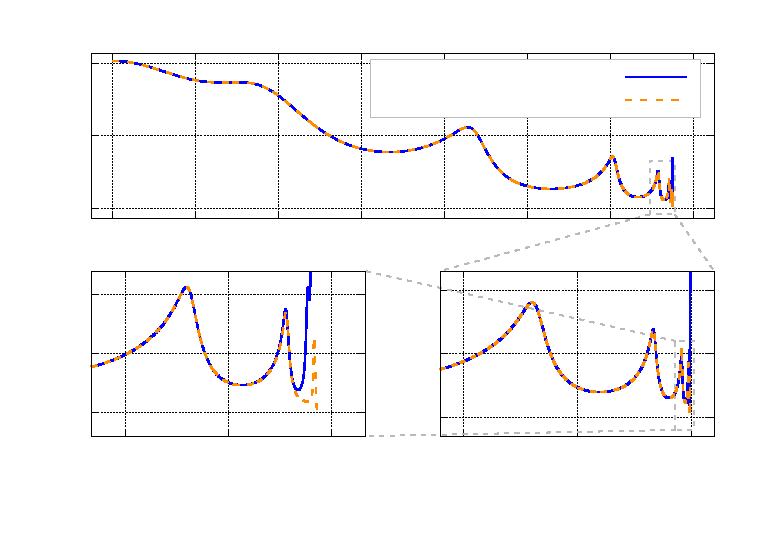
\includegraphics{resources/critical_lapse_v2}}%
    \gplfronttext
  \end{picture}%
\endgroup

  \caption[$\alpha_{\rm central}$ results near criticality using a different grid setup.]{$\alpha_{\rm central}$ results near criticality using a different grid setup. The simulation parameters used were $N_{r}=320$, $w=0.086$, and $r_{\max}=24$. Note that we have fine-tuned the critical parameter to $\d\eta\sim10^{-13}$.}
  \label{fig:critical_alpha_v2}
\end{figure}

\begin{figure}[H]
  \centering
  % GNUPLOT: LaTeX picture with Postscript
\begingroup
  \makeatletter
  \providecommand\color[2][]{%
    \GenericError{(gnuplot) \space\space\space\@spaces}{%
      Package color not loaded in conjunction with
      terminal option `colourtext'%
    }{See the gnuplot documentation for explanation.%
    }{Either use 'blacktext' in gnuplot or load the package
      color.sty in LaTeX.}%
    \renewcommand\color[2][]{}%
  }%
  \providecommand\includegraphics[2][]{%
    \GenericError{(gnuplot) \space\space\space\@spaces}{%
      Package graphicx or graphics not loaded%
    }{See the gnuplot documentation for explanation.%
    }{The gnuplot epslatex terminal needs graphicx.sty or graphics.sty.}%
    \renewcommand\includegraphics[2][]{}%
  }%
  \providecommand\rotatebox[2]{#2}%
  \@ifundefined{ifGPcolor}{%
    \newif\ifGPcolor
    \GPcolorfalse
  }{}%
  \@ifundefined{ifGPblacktext}{%
    \newif\ifGPblacktext
    \GPblacktexttrue
  }{}%
  % define a \g@addto@macro without @ in the name:
  \let\gplgaddtomacro\g@addto@macro
  % define empty templates for all commands taking text:
  \gdef\gplbacktext{}%
  \gdef\gplfronttext{}%
  \makeatother
  \ifGPblacktext
    % no textcolor at all
    \def\colorrgb#1{}%
    \def\colorgray#1{}%
  \else
    % gray or color?
    \ifGPcolor
      \def\colorrgb#1{\color[rgb]{#1}}%
      \def\colorgray#1{\color[gray]{#1}}%
      \expandafter\def\csname LTw\endcsname{\color{white}}%
      \expandafter\def\csname LTb\endcsname{\color{black}}%
      \expandafter\def\csname LTa\endcsname{\color{black}}%
      \expandafter\def\csname LT0\endcsname{\color[rgb]{1,0,0}}%
      \expandafter\def\csname LT1\endcsname{\color[rgb]{0,1,0}}%
      \expandafter\def\csname LT2\endcsname{\color[rgb]{0,0,1}}%
      \expandafter\def\csname LT3\endcsname{\color[rgb]{1,0,1}}%
      \expandafter\def\csname LT4\endcsname{\color[rgb]{0,1,1}}%
      \expandafter\def\csname LT5\endcsname{\color[rgb]{1,1,0}}%
      \expandafter\def\csname LT6\endcsname{\color[rgb]{0,0,0}}%
      \expandafter\def\csname LT7\endcsname{\color[rgb]{1,0.3,0}}%
      \expandafter\def\csname LT8\endcsname{\color[rgb]{0.5,0.5,0.5}}%
    \else
      % gray
      \def\colorrgb#1{\color{black}}%
      \def\colorgray#1{\color[gray]{#1}}%
      \expandafter\def\csname LTw\endcsname{\color{white}}%
      \expandafter\def\csname LTb\endcsname{\color{black}}%
      \expandafter\def\csname LTa\endcsname{\color{black}}%
      \expandafter\def\csname LT0\endcsname{\color{black}}%
      \expandafter\def\csname LT1\endcsname{\color{black}}%
      \expandafter\def\csname LT2\endcsname{\color{black}}%
      \expandafter\def\csname LT3\endcsname{\color{black}}%
      \expandafter\def\csname LT4\endcsname{\color{black}}%
      \expandafter\def\csname LT5\endcsname{\color{black}}%
      \expandafter\def\csname LT6\endcsname{\color{black}}%
      \expandafter\def\csname LT7\endcsname{\color{black}}%
      \expandafter\def\csname LT8\endcsname{\color{black}}%
    \fi
  \fi
    \setlength{\unitlength}{0.0500bp}%
    \ifx\gptboxheight\undefined%
      \newlength{\gptboxheight}%
      \newlength{\gptboxwidth}%
      \newsavebox{\gptboxtext}%
    \fi%
    \setlength{\fboxrule}{0.5pt}%
    \setlength{\fboxsep}{1pt}%
\begin{picture}(7200.00,5040.00)%
    \gplgaddtomacro\gplbacktext{%
      \csname LTb\endcsname%%
      \put(588,3198){\makebox(0,0)[r]{\strut{}0.00}}%
      \csname LTb\endcsname%%
      \put(588,3893){\makebox(0,0)[r]{\strut{}0.35}}%
      \csname LTb\endcsname%%
      \put(588,4587){\makebox(0,0)[r]{\strut{}0.70}}%
      \csname LTb\endcsname%%
      \put(992,2879){\makebox(0,0){\strut{}$0$}}%
      \csname LTb\endcsname%%
      \put(2078,2879){\makebox(0,0){\strut{}$2$}}%
      \csname LTb\endcsname%%
      \put(3164,2879){\makebox(0,0){\strut{}$4$}}%
      \csname LTb\endcsname%%
      \put(4251,2879){\makebox(0,0){\strut{}$6$}}%
      \csname LTb\endcsname%%
      \put(5337,2879){\makebox(0,0){\strut{}$8$}}%
      \csname LTb\endcsname%%
      \put(6423,2879){\makebox(0,0){\strut{}$10$}}%
    }%
    \gplgaddtomacro\gplfronttext{%
      \csname LTb\endcsname%%
      \put(-50,3892){\rotatebox{-270}{\makebox(0,0){\strut{}$\alpha_{\rm central}$}}}%
      \put(3707,569){\makebox(0,0){\strut{}$t$}}%
      \csname LTb\endcsname%%
      \put(5708,4458){\makebox(0,0)[r]{\strut{}$\eta = 0.2914370451806$}}%
      \csname LTb\endcsname%%
      \put(5708,4238){\makebox(0,0)[r]{\strut{}$\eta = 0.2914370451807$}}%
    }%
    \gplgaddtomacro\gplbacktext{%
      \csname LTb\endcsname%%
      \put(3935,1191){\makebox(0,0)[r]{\strut{}0.0}}%
      \csname LTb\endcsname%%
      \put(3935,1802){\makebox(0,0)[r]{\strut{}$0.1$}}%
      \csname LTb\endcsname%%
      \put(3935,2412){\makebox(0,0)[r]{\strut{}$0.2$}}%
      \csname LTb\endcsname%%
      \put(4505,788){\makebox(0,0){\strut{}$9.4$}}%
      \csname LTb\endcsname%%
      \put(5381,788){\makebox(0,0){\strut{}$9.6$}}%
      \csname LTb\endcsname%%
      \put(6257,788){\makebox(0,0){\strut{}$9.8$}}%
    }%
    \gplgaddtomacro\gplfronttext{%
    }%
    \gplgaddtomacro\gplbacktext{%
      \csname LTb\endcsname%%
      \put(588,1235){\makebox(0,0)[r]{\strut{}0.00}}%
      \csname LTb\endcsname%%
      \put(588,1802){\makebox(0,0)[r]{\strut{}$0.05$}}%
      \csname LTb\endcsname%%
      \put(588,2368){\makebox(0,0)[r]{\strut{}0.10}}%
      \csname LTb\endcsname%%
      \put(1048,788){\makebox(0,0){\strut{}$9.854$}}%
      \csname LTb\endcsname%%
      \put(2034,788){\makebox(0,0){\strut{}$9.866$}}%
      \csname LTb\endcsname%%
      \put(3019,788){\makebox(0,0){\strut{}$9.878$}}%
    }%
    \gplgaddtomacro\gplfronttext{%
    }%
    \gplbacktext
    \put(0,0){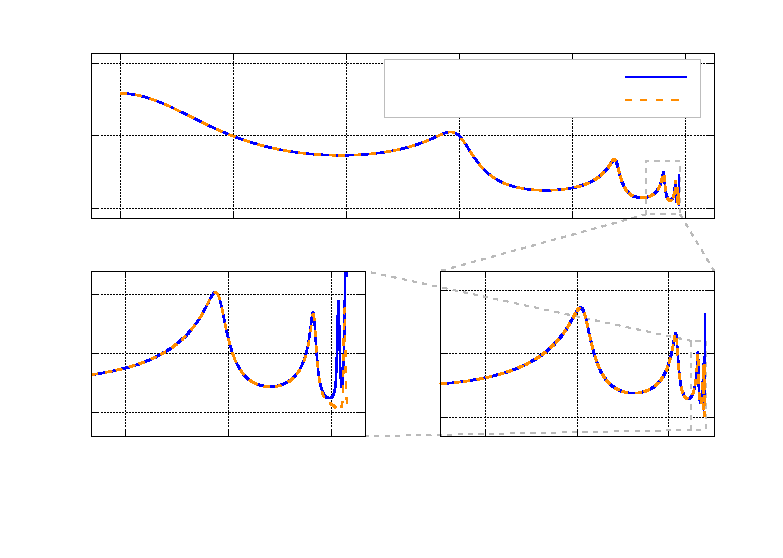
\includegraphics{resources/critical_lapse_tanh}}%
    \gplfronttext
  \end{picture}%
\endgroup

  \caption[$\alpha_{\rm central}$ results near criticality using a different grid setup.]{$\alpha_{\rm central}$ results near criticality using a different grid setup. The simulation parameters used were $N_{r}=320$, $w=0.086$, and $r_{\max}=24$. Note that we have fine-tuned the critical parameter to $\d\eta\sim10^{-13}$.}
  \label{fig:critical_alpha_tanh}
\end{figure}

\setlength{\abovecaptionskip}{16pt plus 0pt minus 0pt}

\begin{figure}[H]
  \centering
  % GNUPLOT: LaTeX picture with Postscript
\begingroup
  \makeatletter
  \providecommand\color[2][]{%
    \GenericError{(gnuplot) \space\space\space\@spaces}{%
      Package color not loaded in conjunction with
      terminal option `colourtext'%
    }{See the gnuplot documentation for explanation.%
    }{Either use 'blacktext' in gnuplot or load the package
      color.sty in LaTeX.}%
    \renewcommand\color[2][]{}%
  }%
  \providecommand\includegraphics[2][]{%
    \GenericError{(gnuplot) \space\space\space\@spaces}{%
      Package graphicx or graphics not loaded%
    }{See the gnuplot documentation for explanation.%
    }{The gnuplot epslatex terminal needs graphicx.sty or graphics.sty.}%
    \renewcommand\includegraphics[2][]{}%
  }%
  \providecommand\rotatebox[2]{#2}%
  \@ifundefined{ifGPcolor}{%
    \newif\ifGPcolor
    \GPcolorfalse
  }{}%
  \@ifundefined{ifGPblacktext}{%
    \newif\ifGPblacktext
    \GPblacktexttrue
  }{}%
  % define a \g@addto@macro without @ in the name:
  \let\gplgaddtomacro\g@addto@macro
  % define empty templates for all commands taking text:
  \gdef\gplbacktext{}%
  \gdef\gplfronttext{}%
  \makeatother
  \ifGPblacktext
    % no textcolor at all
    \def\colorrgb#1{}%
    \def\colorgray#1{}%
  \else
    % gray or color?
    \ifGPcolor
      \def\colorrgb#1{\color[rgb]{#1}}%
      \def\colorgray#1{\color[gray]{#1}}%
      \expandafter\def\csname LTw\endcsname{\color{white}}%
      \expandafter\def\csname LTb\endcsname{\color{black}}%
      \expandafter\def\csname LTa\endcsname{\color{black}}%
      \expandafter\def\csname LT0\endcsname{\color[rgb]{1,0,0}}%
      \expandafter\def\csname LT1\endcsname{\color[rgb]{0,1,0}}%
      \expandafter\def\csname LT2\endcsname{\color[rgb]{0,0,1}}%
      \expandafter\def\csname LT3\endcsname{\color[rgb]{1,0,1}}%
      \expandafter\def\csname LT4\endcsname{\color[rgb]{0,1,1}}%
      \expandafter\def\csname LT5\endcsname{\color[rgb]{1,1,0}}%
      \expandafter\def\csname LT6\endcsname{\color[rgb]{0,0,0}}%
      \expandafter\def\csname LT7\endcsname{\color[rgb]{1,0.3,0}}%
      \expandafter\def\csname LT8\endcsname{\color[rgb]{0.5,0.5,0.5}}%
    \else
      % gray
      \def\colorrgb#1{\color{black}}%
      \def\colorgray#1{\color[gray]{#1}}%
      \expandafter\def\csname LTw\endcsname{\color{white}}%
      \expandafter\def\csname LTb\endcsname{\color{black}}%
      \expandafter\def\csname LTa\endcsname{\color{black}}%
      \expandafter\def\csname LT0\endcsname{\color{black}}%
      \expandafter\def\csname LT1\endcsname{\color{black}}%
      \expandafter\def\csname LT2\endcsname{\color{black}}%
      \expandafter\def\csname LT3\endcsname{\color{black}}%
      \expandafter\def\csname LT4\endcsname{\color{black}}%
      \expandafter\def\csname LT5\endcsname{\color{black}}%
      \expandafter\def\csname LT6\endcsname{\color{black}}%
      \expandafter\def\csname LT7\endcsname{\color{black}}%
      \expandafter\def\csname LT8\endcsname{\color{black}}%
    \fi
  \fi
    \setlength{\unitlength}{0.0500bp}%
    \ifx\gptboxheight\undefined%
      \newlength{\gptboxheight}%
      \newlength{\gptboxwidth}%
      \newsavebox{\gptboxtext}%
    \fi%
    \setlength{\fboxrule}{0.5pt}%
    \setlength{\fboxsep}{1pt}%
\begin{picture}(10080.00,2880.00)%
    \gplgaddtomacro\gplbacktext{%
      \csname LTb\endcsname%%
      \put(876,469){\makebox(0,0)[r]{\strut{}-0.6}}%
      \csname LTb\endcsname%%
      \put(876,831){\makebox(0,0)[r]{\strut{}-0.4}}%
      \csname LTb\endcsname%%
      \put(876,1193){\makebox(0,0)[r]{\strut{}-0.2}}%
      \csname LTb\endcsname%%
      \put(876,1555){\makebox(0,0)[r]{\strut{}0.0}}%
      \csname LTb\endcsname%%
      \put(876,1916){\makebox(0,0)[r]{\strut{}0.2}}%
      \csname LTb\endcsname%%
      \put(876,2278){\makebox(0,0)[r]{\strut{}0.4}}%
      \csname LTb\endcsname%%
      \put(876,2640){\makebox(0,0)[r]{\strut{}0.6}}%
      \csname LTb\endcsname%%
      \put(1378,68){\makebox(0,0){\strut{}$0.0$}}%
      \csname LTb\endcsname%%
      \put(1747,68){\makebox(0,0){\strut{}$0.4$}}%
      \csname LTb\endcsname%%
      \put(2117,68){\makebox(0,0){\strut{}$0.8$}}%
      \csname LTb\endcsname%%
      \put(2486,68){\makebox(0,0){\strut{}$1.2$}}%
      \csname LTb\endcsname%%
      \put(2856,68){\makebox(0,0){\strut{}$1.6$}}%
    }%
    \gplgaddtomacro\gplfronttext{%
      \csname LTb\endcsname%%
      \put(238,1554){\rotatebox{-270}{\makebox(0,0){\strut{}$\psi_{\rm central}$}}}%
    }%
    \gplgaddtomacro\gplbacktext{%
      \csname LTb\endcsname%%
      \put(3093,469){\makebox(0,0)[r]{\strut{}}}%
      \csname LTb\endcsname%%
      \put(3093,831){\makebox(0,0)[r]{\strut{}}}%
      \csname LTb\endcsname%%
      \put(3093,1193){\makebox(0,0)[r]{\strut{}}}%
      \csname LTb\endcsname%%
      \put(3093,1555){\makebox(0,0)[r]{\strut{}}}%
      \csname LTb\endcsname%%
      \put(3093,1916){\makebox(0,0)[r]{\strut{}}}%
      \csname LTb\endcsname%%
      \put(3093,2278){\makebox(0,0)[r]{\strut{}}}%
      \csname LTb\endcsname%%
      \put(3093,2640){\makebox(0,0)[r]{\strut{}}}%
      \csname LTb\endcsname%%
      \put(3595,68){\makebox(0,0){\strut{}$0.0$}}%
      \csname LTb\endcsname%%
      \put(3964,68){\makebox(0,0){\strut{}$0.3$}}%
      \csname LTb\endcsname%%
      \put(4334,68){\makebox(0,0){\strut{}$0.6$}}%
      \csname LTb\endcsname%%
      \put(4703,68){\makebox(0,0){\strut{}$0.9$}}%
      \csname LTb\endcsname%%
      \put(5073,68){\makebox(0,0){\strut{}$1.2$}}%
    }%
    \gplgaddtomacro\gplfronttext{%
      \csname LTb\endcsname%%
      \put(5455,-262){\makebox(0,0){\strut{}$\tau$}}%
    }%
    \gplgaddtomacro\gplbacktext{%
      \csname LTb\endcsname%%
      \put(5311,469){\makebox(0,0)[r]{\strut{}}}%
      \csname LTb\endcsname%%
      \put(5311,831){\makebox(0,0)[r]{\strut{}}}%
      \csname LTb\endcsname%%
      \put(5311,1193){\makebox(0,0)[r]{\strut{}}}%
      \csname LTb\endcsname%%
      \put(5311,1555){\makebox(0,0)[r]{\strut{}}}%
      \csname LTb\endcsname%%
      \put(5311,1916){\makebox(0,0)[r]{\strut{}}}%
      \csname LTb\endcsname%%
      \put(5311,2278){\makebox(0,0)[r]{\strut{}}}%
      \csname LTb\endcsname%%
      \put(5311,2640){\makebox(0,0)[r]{\strut{}}}%
      \csname LTb\endcsname%%
      \put(5760,68){\makebox(0,0){\strut{}$0$}}%
      \csname LTb\endcsname%%
      \put(6076,68){\makebox(0,0){\strut{}$1$}}%
      \csname LTb\endcsname%%
      \put(6393,68){\makebox(0,0){\strut{}$2$}}%
      \csname LTb\endcsname%%
      \put(6710,68){\makebox(0,0){\strut{}$3$}}%
      \csname LTb\endcsname%%
      \put(7027,68){\makebox(0,0){\strut{}$4$}}%
      \csname LTb\endcsname%%
      \put(7343,68){\makebox(0,0){\strut{}$5$}}%
    }%
    \gplgaddtomacro\gplfronttext{%
    }%
    \gplgaddtomacro\gplbacktext{%
      \csname LTb\endcsname%%
      \put(7528,469){\makebox(0,0)[r]{\strut{}}}%
      \csname LTb\endcsname%%
      \put(7528,831){\makebox(0,0)[r]{\strut{}}}%
      \csname LTb\endcsname%%
      \put(7528,1193){\makebox(0,0)[r]{\strut{}}}%
      \csname LTb\endcsname%%
      \put(7528,1555){\makebox(0,0)[r]{\strut{}}}%
      \csname LTb\endcsname%%
      \put(7528,1916){\makebox(0,0)[r]{\strut{}}}%
      \csname LTb\endcsname%%
      \put(7528,2278){\makebox(0,0)[r]{\strut{}}}%
      \csname LTb\endcsname%%
      \put(7528,2640){\makebox(0,0)[r]{\strut{}}}%
      \csname LTb\endcsname%%
      \put(8030,68){\makebox(0,0){\strut{}$0.0$}}%
      \csname LTb\endcsname%%
      \put(8399,68){\makebox(0,0){\strut{}$0.6$}}%
      \csname LTb\endcsname%%
      \put(8769,68){\makebox(0,0){\strut{}$1.2$}}%
      \csname LTb\endcsname%%
      \put(9138,68){\makebox(0,0){\strut{}$1.8$}}%
      \csname LTb\endcsname%%
      \put(9508,68){\makebox(0,0){\strut{}$2.4$}}%
    }%
    \gplgaddtomacro\gplfronttext{%
    }%
    \gplbacktext
    \put(0,0){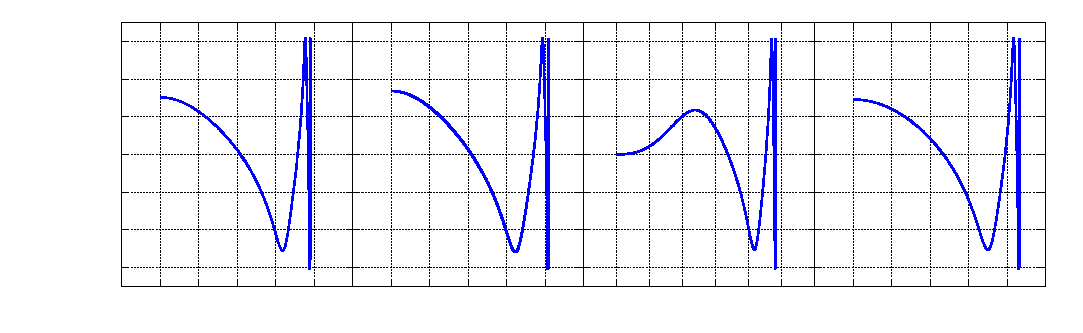
\includegraphics{resources/accumulation_tau_combined}}%
    \gplfronttext
  \end{picture}%
\endgroup

  \caption[$\phi_{\rm central}$ results near criticality for different initial data, as a function of proper time.]{$\phi_{\rm central}$ results near criticality for different initial data, as a function of proper time.}
  \label{fig:accumulation_tau_combined}
\end{figure}

\setlength{\abovecaptionskip}{16pt plus 0pt minus 0pt}

\begin{figure}[H]
  \centering
  % GNUPLOT: LaTeX picture with Postscript
\begingroup
  \makeatletter
  \providecommand\color[2][]{%
    \GenericError{(gnuplot) \space\space\space\@spaces}{%
      Package color not loaded in conjunction with
      terminal option `colourtext'%
    }{See the gnuplot documentation for explanation.%
    }{Either use 'blacktext' in gnuplot or load the package
      color.sty in LaTeX.}%
    \renewcommand\color[2][]{}%
  }%
  \providecommand\includegraphics[2][]{%
    \GenericError{(gnuplot) \space\space\space\@spaces}{%
      Package graphicx or graphics not loaded%
    }{See the gnuplot documentation for explanation.%
    }{The gnuplot epslatex terminal needs graphicx.sty or graphics.sty.}%
    \renewcommand\includegraphics[2][]{}%
  }%
  \providecommand\rotatebox[2]{#2}%
  \@ifundefined{ifGPcolor}{%
    \newif\ifGPcolor
    \GPcolorfalse
  }{}%
  \@ifundefined{ifGPblacktext}{%
    \newif\ifGPblacktext
    \GPblacktexttrue
  }{}%
  % define a \g@addto@macro without @ in the name:
  \let\gplgaddtomacro\g@addto@macro
  % define empty templates for all commands taking text:
  \gdef\gplbacktext{}%
  \gdef\gplfronttext{}%
  \makeatother
  \ifGPblacktext
    % no textcolor at all
    \def\colorrgb#1{}%
    \def\colorgray#1{}%
  \else
    % gray or color?
    \ifGPcolor
      \def\colorrgb#1{\color[rgb]{#1}}%
      \def\colorgray#1{\color[gray]{#1}}%
      \expandafter\def\csname LTw\endcsname{\color{white}}%
      \expandafter\def\csname LTb\endcsname{\color{black}}%
      \expandafter\def\csname LTa\endcsname{\color{black}}%
      \expandafter\def\csname LT0\endcsname{\color[rgb]{1,0,0}}%
      \expandafter\def\csname LT1\endcsname{\color[rgb]{0,1,0}}%
      \expandafter\def\csname LT2\endcsname{\color[rgb]{0,0,1}}%
      \expandafter\def\csname LT3\endcsname{\color[rgb]{1,0,1}}%
      \expandafter\def\csname LT4\endcsname{\color[rgb]{0,1,1}}%
      \expandafter\def\csname LT5\endcsname{\color[rgb]{1,1,0}}%
      \expandafter\def\csname LT6\endcsname{\color[rgb]{0,0,0}}%
      \expandafter\def\csname LT7\endcsname{\color[rgb]{1,0.3,0}}%
      \expandafter\def\csname LT8\endcsname{\color[rgb]{0.5,0.5,0.5}}%
    \else
      % gray
      \def\colorrgb#1{\color{black}}%
      \def\colorgray#1{\color[gray]{#1}}%
      \expandafter\def\csname LTw\endcsname{\color{white}}%
      \expandafter\def\csname LTb\endcsname{\color{black}}%
      \expandafter\def\csname LTa\endcsname{\color{black}}%
      \expandafter\def\csname LT0\endcsname{\color{black}}%
      \expandafter\def\csname LT1\endcsname{\color{black}}%
      \expandafter\def\csname LT2\endcsname{\color{black}}%
      \expandafter\def\csname LT3\endcsname{\color{black}}%
      \expandafter\def\csname LT4\endcsname{\color{black}}%
      \expandafter\def\csname LT5\endcsname{\color{black}}%
      \expandafter\def\csname LT6\endcsname{\color{black}}%
      \expandafter\def\csname LT7\endcsname{\color{black}}%
      \expandafter\def\csname LT8\endcsname{\color{black}}%
    \fi
  \fi
    \setlength{\unitlength}{0.0500bp}%
    \ifx\gptboxheight\undefined%
      \newlength{\gptboxheight}%
      \newlength{\gptboxwidth}%
      \newsavebox{\gptboxtext}%
    \fi%
    \setlength{\fboxrule}{0.5pt}%
    \setlength{\fboxsep}{1pt}%
\begin{picture}(10080.00,2880.00)%
    \gplgaddtomacro\gplbacktext{%
      \csname LTb\endcsname%%
      \put(876,469){\makebox(0,0)[r]{\strut{}$-0.6$}}%
      \csname LTb\endcsname%%
      \put(876,831){\makebox(0,0)[r]{\strut{}$-0.4$}}%
      \csname LTb\endcsname%%
      \put(876,1193){\makebox(0,0)[r]{\strut{}$-0.2$}}%
      \csname LTb\endcsname%%
      \put(876,1555){\makebox(0,0)[r]{\strut{}$0.0$}}%
      \csname LTb\endcsname%%
      \put(876,1916){\makebox(0,0)[r]{\strut{}$0.2$}}%
      \csname LTb\endcsname%%
      \put(876,2278){\makebox(0,0)[r]{\strut{}$0.4$}}%
      \csname LTb\endcsname%%
      \put(876,2640){\makebox(0,0)[r]{\strut{}$0.6$}}%
      \csname LTb\endcsname%%
      \put(1378,68){\makebox(0,0){\strut{}$0$}}%
      \csname LTb\endcsname%%
      \put(1747,68){\makebox(0,0){\strut{}$2$}}%
      \csname LTb\endcsname%%
      \put(2117,68){\makebox(0,0){\strut{}$4$}}%
      \csname LTb\endcsname%%
      \put(2486,68){\makebox(0,0){\strut{}$6$}}%
      \csname LTb\endcsname%%
      \put(2856,68){\makebox(0,0){\strut{}$8$}}%
    }%
    \gplgaddtomacro\gplfronttext{%
      \csname LTb\endcsname%%
      \put(238,1554){\rotatebox{-270}{\makebox(0,0){\strut{}$\psi_{\rm central}$}}}%
    }%
    \gplgaddtomacro\gplbacktext{%
      \csname LTb\endcsname%%
      \put(3093,469){\makebox(0,0)[r]{\strut{}}}%
      \csname LTb\endcsname%%
      \put(3093,831){\makebox(0,0)[r]{\strut{}}}%
      \csname LTb\endcsname%%
      \put(3093,1193){\makebox(0,0)[r]{\strut{}}}%
      \csname LTb\endcsname%%
      \put(3093,1555){\makebox(0,0)[r]{\strut{}}}%
      \csname LTb\endcsname%%
      \put(3093,1916){\makebox(0,0)[r]{\strut{}}}%
      \csname LTb\endcsname%%
      \put(3093,2278){\makebox(0,0)[r]{\strut{}}}%
      \csname LTb\endcsname%%
      \put(3093,2640){\makebox(0,0)[r]{\strut{}}}%
      \csname LTb\endcsname%%
      \put(3542,68){\makebox(0,0){\strut{}$0.0$}}%
      \csname LTb\endcsname%%
      \put(3938,68){\makebox(0,0){\strut{}$2.5$}}%
      \csname LTb\endcsname%%
      \put(4334,68){\makebox(0,0){\strut{}$5.0$}}%
      \csname LTb\endcsname%%
      \put(4729,68){\makebox(0,0){\strut{}$7.5$}}%
      \csname LTb\endcsname%%
      \put(5125,68){\makebox(0,0){\strut{}$10.0$}}%
    }%
    \gplgaddtomacro\gplfronttext{%
      \csname LTb\endcsname%%
      \put(5455,-262){\makebox(0,0){\strut{}$\Lambda$}}%
    }%
    \gplgaddtomacro\gplbacktext{%
      \csname LTb\endcsname%%
      \put(5311,469){\makebox(0,0)[r]{\strut{}}}%
      \csname LTb\endcsname%%
      \put(5311,831){\makebox(0,0)[r]{\strut{}}}%
      \csname LTb\endcsname%%
      \put(5311,1193){\makebox(0,0)[r]{\strut{}}}%
      \csname LTb\endcsname%%
      \put(5311,1555){\makebox(0,0)[r]{\strut{}}}%
      \csname LTb\endcsname%%
      \put(5311,1916){\makebox(0,0)[r]{\strut{}}}%
      \csname LTb\endcsname%%
      \put(5311,2278){\makebox(0,0)[r]{\strut{}}}%
      \csname LTb\endcsname%%
      \put(5311,2640){\makebox(0,0)[r]{\strut{}}}%
      \csname LTb\endcsname%%
      \put(5760,68){\makebox(0,0){\strut{}$0.0$}}%
      \csname LTb\endcsname%%
      \put(6156,68){\makebox(0,0){\strut{}$2.5$}}%
      \csname LTb\endcsname%%
      \put(6552,68){\makebox(0,0){\strut{}$5.0$}}%
      \csname LTb\endcsname%%
      \put(6947,68){\makebox(0,0){\strut{}$7.5$}}%
      \csname LTb\endcsname%%
      \put(7343,68){\makebox(0,0){\strut{}$10.0$}}%
    }%
    \gplgaddtomacro\gplfronttext{%
    }%
    \gplgaddtomacro\gplbacktext{%
      \csname LTb\endcsname%%
      \put(7528,469){\makebox(0,0)[r]{\strut{}}}%
      \csname LTb\endcsname%%
      \put(7528,831){\makebox(0,0)[r]{\strut{}}}%
      \csname LTb\endcsname%%
      \put(7528,1193){\makebox(0,0)[r]{\strut{}}}%
      \csname LTb\endcsname%%
      \put(7528,1555){\makebox(0,0)[r]{\strut{}}}%
      \csname LTb\endcsname%%
      \put(7528,1916){\makebox(0,0)[r]{\strut{}}}%
      \csname LTb\endcsname%%
      \put(7528,2278){\makebox(0,0)[r]{\strut{}}}%
      \csname LTb\endcsname%%
      \put(7528,2640){\makebox(0,0)[r]{\strut{}}}%
      \csname LTb\endcsname%%
      \put(7977,68){\makebox(0,0){\strut{}$0.0$}}%
      \csname LTb\endcsname%%
      \put(8373,68){\makebox(0,0){\strut{}$2.5$}}%
      \csname LTb\endcsname%%
      \put(8769,68){\makebox(0,0){\strut{}$5.0$}}%
      \csname LTb\endcsname%%
      \put(9164,68){\makebox(0,0){\strut{}$7.5$}}%
      \csname LTb\endcsname%%
      \put(9560,68){\makebox(0,0){\strut{}$10.0$}}%
    }%
    \gplgaddtomacro\gplfronttext{%
    }%
    \gplbacktext
    \put(0,0){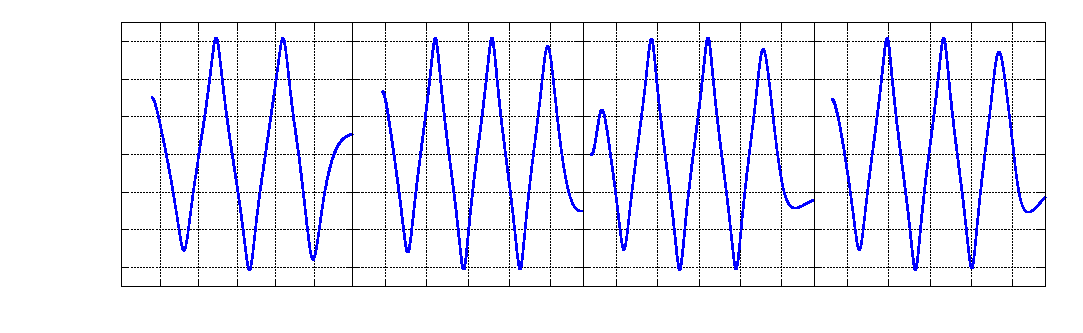
\includegraphics{resources/accumulation_Lambda_combined}}%
    \gplfronttext
  \end{picture}%
\endgroup

  \caption[$\phi_{\rm central}$ results near criticality for different initial data, as a function of logarithmic proper time.]{$\phi_{\rm central}$ results near criticality for different initial data, as a function of logarithmic proper time.}
  \label{fig:accumulation_Lambda_combined}
\end{figure}

\setlength{\abovecaptionskip}{10pt plus 0pt minus 0pt}

\begin{figure}[H]
  \centering
  % GNUPLOT: LaTeX picture with Postscript
\begingroup
  \makeatletter
  \providecommand\color[2][]{%
    \GenericError{(gnuplot) \space\space\space\@spaces}{%
      Package color not loaded in conjunction with
      terminal option `colourtext'%
    }{See the gnuplot documentation for explanation.%
    }{Either use 'blacktext' in gnuplot or load the package
      color.sty in LaTeX.}%
    \renewcommand\color[2][]{}%
  }%
  \providecommand\includegraphics[2][]{%
    \GenericError{(gnuplot) \space\space\space\@spaces}{%
      Package graphicx or graphics not loaded%
    }{See the gnuplot documentation for explanation.%
    }{The gnuplot epslatex terminal needs graphicx.sty or graphics.sty.}%
    \renewcommand\includegraphics[2][]{}%
  }%
  \providecommand\rotatebox[2]{#2}%
  \@ifundefined{ifGPcolor}{%
    \newif\ifGPcolor
    \GPcolorfalse
  }{}%
  \@ifundefined{ifGPblacktext}{%
    \newif\ifGPblacktext
    \GPblacktexttrue
  }{}%
  % define a \g@addto@macro without @ in the name:
  \let\gplgaddtomacro\g@addto@macro
  % define empty templates for all commands taking text:
  \gdef\gplbacktext{}%
  \gdef\gplfronttext{}%
  \makeatother
  \ifGPblacktext
    % no textcolor at all
    \def\colorrgb#1{}%
    \def\colorgray#1{}%
  \else
    % gray or color?
    \ifGPcolor
      \def\colorrgb#1{\color[rgb]{#1}}%
      \def\colorgray#1{\color[gray]{#1}}%
      \expandafter\def\csname LTw\endcsname{\color{white}}%
      \expandafter\def\csname LTb\endcsname{\color{black}}%
      \expandafter\def\csname LTa\endcsname{\color{black}}%
      \expandafter\def\csname LT0\endcsname{\color[rgb]{1,0,0}}%
      \expandafter\def\csname LT1\endcsname{\color[rgb]{0,1,0}}%
      \expandafter\def\csname LT2\endcsname{\color[rgb]{0,0,1}}%
      \expandafter\def\csname LT3\endcsname{\color[rgb]{1,0,1}}%
      \expandafter\def\csname LT4\endcsname{\color[rgb]{0,1,1}}%
      \expandafter\def\csname LT5\endcsname{\color[rgb]{1,1,0}}%
      \expandafter\def\csname LT6\endcsname{\color[rgb]{0,0,0}}%
      \expandafter\def\csname LT7\endcsname{\color[rgb]{1,0.3,0}}%
      \expandafter\def\csname LT8\endcsname{\color[rgb]{0.5,0.5,0.5}}%
    \else
      % gray
      \def\colorrgb#1{\color{black}}%
      \def\colorgray#1{\color[gray]{#1}}%
      \expandafter\def\csname LTw\endcsname{\color{white}}%
      \expandafter\def\csname LTb\endcsname{\color{black}}%
      \expandafter\def\csname LTa\endcsname{\color{black}}%
      \expandafter\def\csname LT0\endcsname{\color{black}}%
      \expandafter\def\csname LT1\endcsname{\color{black}}%
      \expandafter\def\csname LT2\endcsname{\color{black}}%
      \expandafter\def\csname LT3\endcsname{\color{black}}%
      \expandafter\def\csname LT4\endcsname{\color{black}}%
      \expandafter\def\csname LT5\endcsname{\color{black}}%
      \expandafter\def\csname LT6\endcsname{\color{black}}%
      \expandafter\def\csname LT7\endcsname{\color{black}}%
      \expandafter\def\csname LT8\endcsname{\color{black}}%
    \fi
  \fi
    \setlength{\unitlength}{0.0500bp}%
    \ifx\gptboxheight\undefined%
      \newlength{\gptboxheight}%
      \newlength{\gptboxwidth}%
      \newsavebox{\gptboxtext}%
    \fi%
    \setlength{\fboxrule}{0.5pt}%
    \setlength{\fboxsep}{1pt}%
\begin{picture}(7200.00,5040.00)%
    \gplgaddtomacro\gplbacktext{%
      \csname LTb\endcsname%%
      \put(682,1047){\makebox(0,0)[r]{\strut{}$0$}}%
      \csname LTb\endcsname%%
      \put(682,1904){\makebox(0,0)[r]{\strut{}$5$}}%
      \csname LTb\endcsname%%
      \put(682,2762){\makebox(0,0)[r]{\strut{}$10$}}%
      \csname LTb\endcsname%%
      \put(682,3619){\makebox(0,0)[r]{\strut{}$15$}}%
      \csname LTb\endcsname%%
      \put(682,4476){\makebox(0,0)[r]{\strut{}$20$}}%
      \csname LTb\endcsname%%
      \put(1812,484){\makebox(0,0){\strut{}$-30$}}%
      \csname LTb\endcsname%%
      \put(2810,484){\makebox(0,0){\strut{}$-25$}}%
      \csname LTb\endcsname%%
      \put(3809,484){\makebox(0,0){\strut{}$-20$}}%
      \csname LTb\endcsname%%
      \put(4807,484){\makebox(0,0){\strut{}$-15$}}%
      \csname LTb\endcsname%%
      \put(5805,484){\makebox(0,0){\strut{}$-10$}}%
    }%
    \gplgaddtomacro\gplfronttext{%
      \csname LTb\endcsname%%
      \put(308,2761){\rotatebox{-270}{\makebox(0,0){\strut{}$\ln\left(\rho^{\max}_{\rm central}\right)$}}}%
      \put(3808,154){\makebox(0,0){\strut{}$\ln\left(\eta_{*}-\eta\right)$}}%
      \csname LTb\endcsname%%
      \put(5816,4536){\makebox(0,0)[r]{\strut{}BSSN/I}}%
      \csname LTb\endcsname%%
      \put(5816,4316){\makebox(0,0)[r]{\strut{}ADM/I}}%
      \csname LTb\endcsname%%
      \put(5816,4096){\makebox(0,0)[r]{\strut{}ADM/II}}%
      \csname LTb\endcsname%%
      \put(5816,3876){\makebox(0,0)[r]{\strut{}ADM/III}}%
    }%
    \gplbacktext
    \put(0,0){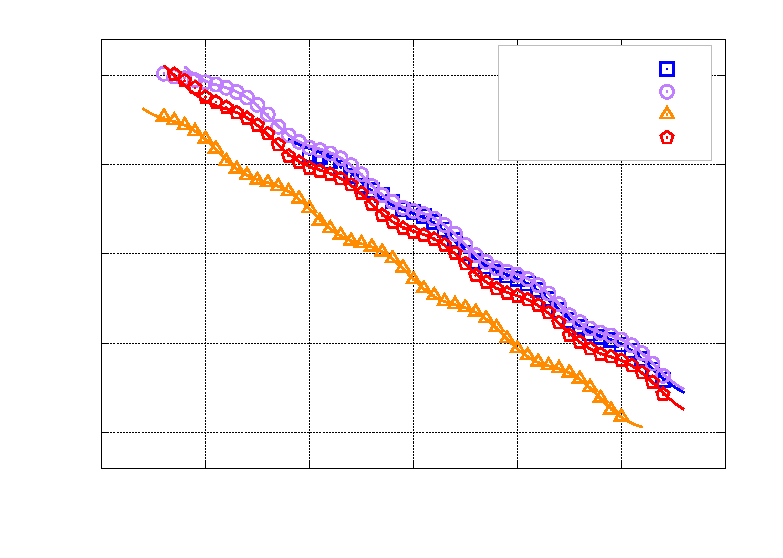
\includegraphics{resources/critical_exponent_combined}}%
    \gplfronttext
  \end{picture}%
\endgroup

  \caption[Central energy density near criticality for different initial data.]{The plot shows the maximum central density for several subcritical runs for different initial data.}
  \label{fig:critical_exponent}
\end{figure}

\al{
  \phi(0,r) &= \eta\exp\lrpar{-\frac{r^{2}}{\d^{2}}}\ ,\label{eq:ic_1}\\
  \phi(0,r) &= \eta\,r^{3}\,\exp\lrsquare{-\lrpar{\frac{r-r_{0}}{\d}}^{2}}\ ,\label{eq:ic_2}\\
  \phi(0,r) &= \eta\lrcurly{1 - \tanh\lrsquare{\lrpar{\frac{r-r_{0}}{\d}}^{2}}}\ .\label{eq:ic_3}
}

$$
\nabla_{\mu}\lrpar{\nabla^{\mu}\phi}=0\ .
$$

% Print the references on a new page
\clearpage
\spacing{1.0}
\printbibliography

\end{document}
% .---------------------------.
% |    End of the document    |
% .---------------------------.
